%% ============================================================================
%% Third revision (R3), Information Processing and Management
%% An Automated Confidence-Aware Framework for Sarcasm Detection in App Reviews
%% Using Inference-Optimized Transformer Language Models
%%
%% Tracked version: every change is labelled with the reviewer comment it
%% answers (R5C1 to R5C12, R7C1 to R7C7). Set \trackedfalse for the clean file.
%% ============================================================================
\documentclass[a4paper,fleqn]{cas-sc}

\usepackage[authoryear,longnamesfirst]{natbib}
\usepackage{amsmath,amssymb}
\usepackage{booktabs,multirow,array,makecell}
\usepackage{graphicx}
\usepackage{xcolor}
\usepackage{algorithm}
\usepackage{algpseudocode}
\usepackage[most]{tcolorbox}
\usepackage{adjustbox}
%% Figures are found next to this file or in a subfolder named manuscript/.
\graphicspath{{./}{manuscript/}}

%% ===========================================================================
%% Revision tracking for the third revision (R3)
%%
%% Every change is labelled with the identifier of the reviewer comment that
%% motivated it, for example R5C4 (Reviewer 5, Comment 4) or R7C3 (Reviewer 7,
%% Comment 3). The colour shows whose comment it answers:
%%   blue    Reviewer 5
%%   red     Reviewer 7
%%   purple  a concern raised by both reviewers (identifiers of both are given)
%%   green   copy-editing, grammar and terminology (R7C7)
%% Inserted text is coloured; deleted text is coloured and struck through.
%%
%%   \rc{IDs}{text}         inserted or rewritten text
%%   \rcdel{IDs}{text}      deleted text (vanishes in the clean version)
%%   \rcrep{IDs}{old}{new}  replaced text
%%   \rce{text}             copy-editing (R7C7), colour only, no label
%%   \rcx{IDs}{text}        as \rc, for headings and captions (no page record)
%%   \rcmark{IDs}           records the page for IDs without printing anything
%%   \rcnote{IDs}{note}     explanatory note shown only in the tracked version
%%   \rcm{IDs}{math}        colours an equation without a label
%%   \begin{rcblock}{IDs} ... \end{rcblock}   whole new paragraphs
%%
%% \trackedtrue produces the tracked manuscript, \trackedfalse the clean one.
%% Each use records its page, so \rvpages{ID} lists every page on which a
%% comment was addressed (used by the index of revisions and by the response).
%% ===========================================================================
\usepackage{etoolbox}
\usepackage{xstring}
\usepackage{refcount}
\newif\iftracked
%% A little extra stretch lets lines that contain tags and struck text break cleanly.
\setlength{\emergencystretch}{1.5em}
\definecolor{rvFive}{HTML}{1F4FBF}
\definecolor{rvSeven}{HTML}{B3261E}
\definecolor{rvBoth}{HTML}{7A2E8E}
\definecolor{rvEdit}{HTML}{1A7D3B}
\makeatletter
%% Strike-through: ulem where it is installed (Overleaf and full TeX Live),
%% otherwise a word-by-word rule so that previews still show deletions.
\def\rv@sw#1{\setbox\z@\hbox{#1}\rlap{\rule[0.55ex]{\wd\z@}{0.5pt}}\box\z@}
\def\rv@sl#1 #2\rv@end{\rv@sw{#1}\if\relax\detokenize{#2}\relax\else\space\rv@sl#2\rv@end\fi}
\newcommand{\rv@fallbackstrike}[1]{\rv@sl#1 \rv@end}
\IfFileExists{ulem.sty}{\RequirePackage[normalem]{ulem}\let\rv@strike\sout}{\let\rv@strike\rv@fallbackstrike}
\newcommand{\rv@setcolour}[1]{%
  \IfStrEq{#1}{R7C7}{\color{rvEdit}}{%
    \IfSubStr{#1}{R5}{\IfSubStr{#1}{R7}{\color{rvBoth}}{\color{rvFive}}}{\color{rvSeven}}}}
\newcommand{\rv@tag}[1]{\textsuperscript{\sffamily\bfseries\scriptsize[\StrSubstitute{#1}{,}{, }]}\,}
\newcommand{\rv@recordone}[1]{%
  \edef\rv@i{#1}%
  \ifcsdef{rv@n@\rv@i}{}{\csgdef{rv@n@\rv@i}{0}}%
  \csxdef{rv@n@\rv@i}{\the\numexpr\csuse{rv@n@\rv@i}+1\relax}%
  \begingroup\edef\@currentlabel{\rv@i}\label{rv:\rv@i:\csuse{rv@n@\rv@i}}\endgroup}
\newcommand{\rv@record}[1]{\@for\rv@id:=#1\do{\expandafter\rv@recordone\expandafter{\rv@id}}}
\DeclareRobustCommand{\rc}[2]{\rv@record{#1}\iftracked{\rv@setcolour{#1}\rv@tag{#1}#2}\else#2\fi}
\DeclareRobustCommand{\rcx}[2]{\iftracked{\rv@setcolour{#1}\rv@tag{#1}#2}\else#2\fi}
\DeclareRobustCommand{\rcmark}[1]{\rv@record{#1}}
\DeclareRobustCommand{\rcdel}[2]{\rv@record{#1}\iftracked{\rv@setcolour{#1}\rv@tag{#1}\rv@strike{#2}}\else\unskip\fi}
\DeclareRobustCommand{\rcrep}[3]{\rv@record{#1}\iftracked{\rv@setcolour{#1}\rv@tag{#1}\rv@strike{#2} #3}\else#3\fi}
\DeclareRobustCommand{\rce}[1]{\rv@record{R7C7}\iftracked{\color{rvEdit}#1}\else#1\fi}
\DeclareRobustCommand{\rcm}[2]{\iftracked{\rv@setcolour{#1}#2}\else#2\fi}
\DeclareRobustCommand{\rvstrikeplain}[1]{\rv@strike{#1}}
\DeclareRobustCommand{\rcnote}[2]{\rv@record{#1}\iftracked{\rv@setcolour{#1}\rv@tag{#1}\textit{[#2]}}\else\unskip\fi}
\newenvironment{rcblock}[1]{\rv@record{#1}\iftracked\rv@setcolour{#1}\leavevmode\rv@tag{#1}\fi\ignorespaces}{\par}
\makeatother

%% Pages on which a comment was addressed, for example "pp. 2, 7 and 31".
%% The optional argument is a label prefix (M- when read through xr).
\ExplSyntaxOn
\seq_new:N \l__rv_pages_seq
\int_new:N \l__rv_n_int
\tl_new:N \l__rv_page_tl
\NewDocumentCommand{\rvpages}{O{}m}{
  \seq_clear:N \l__rv_pages_seq
  %% Labels can be numbered with gaps when a box is typeset on trial and
  %% discarded, so every number up to the limit is examined.
  \int_step_inline:nnn {1} {999}
    {
      \cs_if_exist:cT { r@#1rv:#2:##1 }
        {
          \tl_set:Nx \l__rv_page_tl { \getpagerefnumber{#1rv:#2:##1} }
          \seq_if_in:NVF \l__rv_pages_seq \l__rv_page_tl
            { \seq_put_right:NV \l__rv_pages_seq \l__rv_page_tl }
        }
    }
  \seq_sort:Nn \l__rv_pages_seq
    { \int_compare:nNnTF {##1} > {##2} { \sort_return_swapped: } { \sort_return_same: } }
  \seq_if_empty:NTF \l__rv_pages_seq
    { (compile~twice) }
    {
      \int_compare:nNnTF { \seq_count:N \l__rv_pages_seq } = {1} { p.\nobreakspace } { pp.\nobreakspace }
      \seq_use:Nnnn \l__rv_pages_seq { ~and~ } { ,~ } { ~and~ }
    }
}
\ExplSyntaxOff


\trackedtrue   % \trackedfalse produces the clean manuscript

\newtcolorbox{keyfinding}[1]{colback=blue!3!white,colframe=black,fonttitle=\bfseries,
  title={#1},arc=1.5mm,boxrule=0.8pt,left=2mm,right=2mm,breakable}
\newtcolorbox{rqbox}{colback=gray!8!white,colframe=gray!60,arc=1.5mm,boxrule=0.6pt,left=2mm,right=2mm}
\newtcolorbox{examplebox}[1]{colback=white,colframe=black,fonttitle=\bfseries,title={#1},
  arc=1.5mm,boxrule=0.8pt,left=2mm,right=2mm,breakable}

\begin{document}
\let\WriteBookmarks\relax
\def\floatpagepagefraction{1}
\def\textpagefraction{.001}

%% R5C1, R7C5: the running header previously read "Sarcasm Identification from App Reviews using an Agentic AI".
\shorttitle{Confidence-aware sarcasm detection in app reviews}
\shortauthors{B Shahid et al.}

%% The PDF metadata receives the plain title through \texorpdfstring, because
%% the Elsevier class copies the title into the PDF properties.
\title [mode = title]{\texorpdfstring{\iftracked\rcx{R5C1,R7C5}{\rvstrikeplain{An Agentic Framework For Sarcasm Detection in App Reviews Using Inference-Optimized Transformer Language Model}}\\ \fi\rcx{R5C1,R7C5}{An Automated Confidence-Aware Framework for Sarcasm Detection in App Reviews Using Inference-Optimized Transformer Language Models}}{An Automated Confidence-Aware Framework for Sarcasm Detection in App Reviews Using Inference-Optimized Transformer Language Models}}

%% Author and affiliation block: paste the block of the submitted source here unchanged.
\cortext[cor1]{Corresponding author}

\rcmark{R5C1,R7C5}%
\begin{abstract}
Sarcasm in mobile app reviews poses a significant challenge for sentiment analysis, as the intended meaning often contradicts the literal expression, leading to misleading interpretations in software analytics. While prior research has extensively explored sarcasm detection in social media, domain-specific investigation in app reviews remains limited. This study aims to develop and evaluate an efficient transformer-based framework for sarcasm detection and fine-grained classification in mobile app reviews. We conduct an empirical analysis on a publicly available benchmark corpus of 10,000 manually annotated Google Play Store reviews, drawn from a larger scraped collection of approximately 55,000 reviews. Two separate classification tasks are defined over this corpus: a binary task that distinguishes sarcastic from non-sarcastic reviews over 9,999 annotated reviews, and a sarcasm-type task that classifies \rcrep{R5C9,R7C2}{the 3,460 sarcastic reviews}{3,460 reviews annotated with a sarcasm type} into five categories, namely humor, irony, flattery, self-deprecation, and passive aggression. Five Transformer Language Models (BERT, RoBERTa, DistilBERT, TinyBERT, and MiniLM) are fine-tuned and evaluated on held-out test partitions across three random seeds. Averaged over seeds, BERT and DistilBERT achieve a Macro F1-score of 0.9941 on the binary task, and BERT achieves a Macro F1-score of 0.8301 on the sarcasm-type task. Paired bootstrap and McNemar testing \rc{R5C10}{with Holm correction for multiple comparisons} shows that TinyBERT performs significantly worse than \rcrep{R5C10}{the other four architectures}{BERT and DistilBERT} on both tasks, while \rcrep{R5C10}{the differences among BERT, RoBERTa, DistilBERT, and MiniLM are not statistically distinguishable across seeds}{no difference among BERT, RoBERTa, DistilBERT, and MiniLM survives the correction}. \rc{R5C9,R7C2}{Because the benchmark contains repeated reviews and 230 reviews annotated with two different sarcasm types, both datasets were also deduplicated before partitioning and all encoder experiments were repeated, which gives a best mean Macro F1-score of 0.9975 on the binary task and 0.9364 on the sarcasm-type task, with the gain on the second task coming mainly from the removal of the conflicting annotations.} \rc{R7C6}{A TF-IDF logistic regression baseline reaches a Macro F1-score of 0.9673 on the binary task, which shows that the binary class boundary of this benchmark is largely lexical.} In two dedicated controlled experiments in which the attention backend was verified at runtime, FlashAttention reduces training time by 5.4\% to 21.9\% and inference latency by 3.4\% to 27.2\% across both tasks, while leaving predictive performance materially unchanged. Peak GPU training memory falls by 10.2\% to 18.1\% in the sarcasm-type experiment, which uses the FlashAttention-2 library, but is essentially unchanged in the binary experiment, which uses the PyTorch scaled dot-product attention FlashAttention backend. These results indicate that the contribution of FlashAttention in this setting is computational rather than predictive, and that its memory benefit depends on the specific implementation employed. \rcrep{R5C2}{Then evaluated zero-shot Mistral (Mistral-7B-Instruct-v0.3) baseline performs}{The evaluated zero-shot Mistral-7B-Instruct-v0.3 baseline performs} substantially below the fine-tuned encoder models on both tasks. The framework is deployed within an automated, confidence-aware orchestration pipeline that ingests new app reviews, routes low-confidence predictions for additional processing, and synchronizes results with a cloud-based workflow without autonomous planning or goal generation. \rc{R7C3}{On the deduplicated test partitions the confidence scores that drive this routing are well calibrated, with an expected calibration error of at most 0.022, and routed sarcasm-type predictions are far less accurate than accepted ones, although most errors are made with high confidence and therefore pass the threshold.} These findings indicate that combining fine-tuned transformer modelling, verified efficiency optimization, and automated workflow orchestration can support practical sarcasm-aware analysis of app reviews.\rcdel{R5C2}{for app review analytics.}
\end{abstract}

\begin{keywords}
Sentiment Analysis \sep App Review Analytics \sep MSR \sep BERT \sep CrowdRE \sep Transformer Architecture \sep LLMs \sep \rcrep{R5C1,R7C5}{Agentic AI}{FlashAttention} \sep \rc{R5C1,R7C5}{Confidence-Based Routing}
\end{keywords}

\maketitle

\iftracked
\begin{tcolorbox}[colback=white,colframe=black!70,arc=1.5mm,boxrule=0.6pt,left=2mm,right=2mm,
  fonttitle=\bfseries,title={Guide to the tracked changes of the third revision}]
\small This version marks every change made in response to the third round of review. Each change carries the identifier of the comment that it answers, so that \textbf{[R5C4]} refers to Comment~4 of Reviewer~5 and \textbf{[R7C3]} to Comment~3 of Reviewer~7, and the same identifiers are used throughout the response letter. {\color{rvFive}\textbf{Blue}} text answers Reviewer~5, {\color{rvSeven}\textbf{red}} text answers Reviewer~7, and {\color{rvBoth}\textbf{purple}} text answers a concern that both reviewers raised, in which case the identifiers of both comments are given. {\color{rvEdit}\textbf{Green}} text without a label is copy-editing of grammar, terminology and cross-references in response to the readability remarks of both reviewers, recorded as R7C7. Deleted text is struck through in the colour of the comment that motivated its removal. The merging of duplicate references (R5C12) changes many in-text citations, for example Devlin et al. (2019a) becoming Devlin et al. (2019), and these citation changes are not marked one by one. The running header, which previously read \textit{Sarcasm Identification from App Reviews using an Agentic AI}, has been changed under R5C1 and R7C5. The index at the end of the manuscript lists, for every comment, the pages on which it is addressed.
\end{tcolorbox}
\fi

%% ============================================================================
\section{Introduction}
\label{sec:intro}

In today's digital ecosystem mobile applications have evolved beyond simple tools for entertainment or productivity; they function as dynamic platforms where millions of users continuously share their experiences, expectations, and frustrations \citep{maalej2015bug,putri2025sarcasm,alam2025automating}. Application marketplaces such as the Google Play Store generate a vast and continuous stream of user reviews, forming an active communication channel between developers and end users \citep{ciurumelea2017analyzing,khan2025exploring}. These reviews have become a valuable resource for software engineering, as they reveal usability issues, functional defects, and evolving user requirements much earlier than traditional feedback mechanisms \citep{delima2024opinion,gambo2024extracting}. Moreover, prior studies indicate that user-generated reviews are often more candid and emotionally expressive than structured surveys or controlled experiments \citep{nguyenduc2025generative}.

However\rce{,} this richness also introduces significant analytical challenges. App reviews are inherently unstructured and frequently contain informal language, emojis, abbreviations, and complex linguistic constructs such as sarcasm and exaggeration \citep{haripriya2017survey,wang2024how}. Among these, sarcasm represents one of the most challenging phenomena, as the intended meaning often contradicts the literal expression \citep{veeramani2024harnessing}. For example, a statement such as ``Amazing update, now the app crashes even faster!'' conveys dissatisfaction despite the presence of positive wording \citep{gonzalez2011identifying,celik2025analyzing}. Traditional sentiment analysis approaches, which primarily rely on lexical polarity, often misinterpret such expressions, leading to inaccurate sentiment classification \citep{poria2016deeper}. This misclassification can have serious implications in software analytics, where developers may overlook critical user concerns, resulting in delayed bug fixes, incorrect prioritization, and misguided release decisions \citep{adedigba2025systematic}.

Although sarcasm detection has been extensively studied in Natural Language Processing (NLP), most prior work has focused on social media platforms \citep{gonzalez2011identifying} such as Twitter \citep{poria2016deeper} and Reddit \citep{adedigba2025systematic}. In contrast, app reviews present a distinct and more complex linguistic environment. Compared to short-form social media posts, app reviews are typically longer, more detailed, and often combine emotional expression with technical commentary \citep{veeramani2024harnessing}. A single review may simultaneously include appreciation, criticism, and subtle irony, making sarcasm detection significantly more challenging \citep{haripriya2017survey,adedigba2025systematic}. Despite these differences, domain-specific research on sarcasm detection in app reviews remains limited \citep{maalej2015bug,ciurumelea2017analyzing}. Models trained on social media data often fail to generalize effectively to software-related text due to differences in context, vocabulary, and discourse structure \citep{gambo2024extracting,adedigba2025systematic}.

The emergence of transformer-based language models, such as BERT \citep{devlin2019bert}, RoBERTa \citep{liu2020roberta}, and DistilBERT \citep{sanh2019distilbert}, has significantly advanced sarcasm detection by enabling deep contextual understanding through self-attention mechanisms \citep{vaswani2017attention}. These models are capable of capturing nuanced linguistic patterns, including contradiction, exaggeration, and implicit sentiment. However, deploying Transformer Language Models in large-scale, real-world systems introduces substantial computational challenges \citep{wolf2020transformers}. As app review datasets continue to grow, the quadratic complexity of traditional self-attention mechanisms \citep{brauwers2021general} leads to increased training time and inference latency \citep{dao2024flashattention2}, limiting their practicality in \rcrep{R5C1,R7C5}{real-time}{time-sensitive} analytics environments \citep{rabe2021self}. To address these computational limitations, recent research has introduced FlashAttention \citep{dao2022flashattention}, an input-output-aware attention implementation that reduces memory movement during the attention computation \citep{wolf2020transformers,rabe2021self}. It is important to be precise about what this technique does and does not offer. FlashAttention computes the same attention function as the standard formulation up to floating-point rounding, so it is an optimization of how attention is computed rather than a change to what is computed. Its expected benefits are therefore computational, namely reduced training time, reduced inference latency and, depending on the implementation, reduced peak memory consumption \citep{dao2024flashattention2,liu2023efficientvit}. It is not expected to improve predictive quality, and this study does not treat it as an accuracy-improving mechanism. In software engineering contexts, where feedback must be analysed within continuous integration and deployment cycles, such efficiency improvements are nevertheless valuable because they determine the cost of operating a model at scale.

Efficient inference alone does not make a classifier operationally useful. A sarcasm detection model that is intended to inform software analytics must also be embedded in a process that ingests new reviews, applies the model, handles predictions about which the model is uncertain, and makes the outcome available to developers. Research on AI systems has increasingly described such arrangements using the vocabulary of agentic paradigms \citep{yasmin2025empirical,jiang2026large}, in which models interact with external tools and participate in decision-making. \rcrep{R5C1,R7C5}{That vocabulary spans a wide range of system designs, and we therefore state at the outset, and precisely, what the present work does and does not implement, so that this definition governs the terminology used throughout the manuscript.}{That vocabulary spans a wide range of system designs, and because the present work claims no agentic behaviour of any kind, we state precisely at the outset what it does implement.} The pipeline proposed in this study executes a predefined sequence of six operations: ingestion of new reviews, preprocessing, transformer inference, confidence evaluation, conditional routing of low-confidence predictions, and synchronization of results with a cloud analytics layer. The sequence runs without human intervention at run time and contains exactly one conditional branch, which is governed by a fixed confidence threshold. \rcdel{R5C3}{The pipeline executes a predefined sequence of six operations: review ingestion, preprocessing, transformer inference, confidence evaluation, confidence-based routing, and cloud synchronization. It contains a single predefined conditional branch governed by a fixed confidence threshold.} It does not perform autonomous planning, goal generation, tool selection, strategy selection, or self-reflective reasoning. Accordingly, its automation is limited to workflow orchestration and confidence-conditioned routing. \rcdel{R5C3}{Its automation is therefore confined to orchestration and confidence-conditioned routing.} \rcrep{R5C1,R7C5}{We use the term automated, confidence-aware orchestration pipeline in the technical sections of this manuscript. Where the word agentic appears, including in the title, it denotes only this restricted orchestration and routing behaviour, and it should not be read as a claim of general-purpose autonomous agency.}{For this reason the system is described throughout the manuscript, including its title, as an automated, confidence-aware orchestration pipeline, and the word agentic is used only where we refer to the literature on agentic systems.} No claim of autonomous planning, autonomous tool selection or self-reflective reasoning is made anywhere in this manuscript.

Within this scope, the proposed system detects sarcasm in app reviews, processes newly ingested reviews on a scheduled basis, routes low-confidence predictions for additional processing and flagging, and writes structured labels and aggregated category statistics to a cloud analytics layer that developers can consult. The reduction in inference latency reported in this study supports low-latency processing of incoming reviews, \rcrep{R7C7}{although the framework is integrated into an automated, confidence-aware orchestration pipeline, and}{but the framework was evaluated on an offline benchmark, and} we make no claim of demonstrated production-grade continuous operation.

Despite recent advances in NLP and software analytics, integrating accurate sarcasm detection with efficient computation and a deployable process remains comparatively underexplored. Existing studies primarily evaluate model performance in isolation \citep{savaryleblanc2023software}, with limited attention to scalability \citep{putri2025sarcasm}, low-latency processing, and integration into developer-centric tools \citep{shinn2023reflexion}. To the best of our knowledge, and without claiming the coverage of a systematic literature review, limited attention has been given to jointly evaluating domain-specific sarcasm classification, inference-oriented efficiency optimization, and automated confidence-aware orchestration within a single unified pipeline \citep{yasmin2025empirical,schick2023toolformer,yao2023react,haghsheno2020revolutionizing}.

To address this gap, the present study proposes a transformer-based sarcasm identification framework for mobile app reviews, evaluated with and without an optimized attention implementation and deployed within an automated, confidence-aware orchestration pipeline. The objective is to evaluate predictive effectiveness on both the binary and the fine-grained sarcasm-type task while separately quantifying computational efficiency in terms of training time, inference latency and memory consumption, and to assess the practical applicability of the resulting system for software analytics. Predictive effectiveness and computational efficiency are reported as distinct outcomes throughout this manuscript and are never combined into a single claim of improvement. The remainder of the paper investigates the effectiveness, efficiency and practical applicability of the proposed approach through the research objectives and research questions set out below.

\subsection{Research Objectives}
The primary objective of this study is to develop and evaluate an efficient framework for sarcasm detection in mobile app reviews, addressing predictive effectiveness and computational efficiency as separate concerns. Specifically, this research aims to:
\begin{itemize}
\item \textbf{RO1:} Design and evaluate a transformer-based sarcasm detection framework covering two tasks over the annotated benchmark corpus, namely binary detection of sarcastic against non-sarcastic reviews, and fine-grained five-class classification of \rcrep{R5C9,R7C2}{sarcastic reviews}{reviews annotated with a sarcasm type} into humor, irony, flattery, self-deprecation and passive aggression.
\item \textbf{RO2:} Evaluate and compare five transformer architectures, namely BERT, RoBERTa, DistilBERT, TinyBERT and MiniLM, in capturing the contextual and implicit linguistic cues associated with sarcasm, and assess whether the observed differences between them are statistically supported across repeated runs\rc{R5C10}{, after correction for multiple comparisons,}\rc{R5C9,R7C2}{ and after the removal of duplicated and conflicting annotations}.
\item \textbf{RO3:} Evaluate the effect of an optimized FlashAttention implementation by measuring training time, inference latency, peak GPU memory consumption and predictive performance under a runtime-verified attention backend, reporting the computational and predictive effects separately.
\item \textbf{RO4:} Develop an automated, confidence-aware orchestration pipeline that processes newly ingested reviews through confidence-based routing of uncertain predictions and synchronization with cloud-based tools, without autonomous planning or goal generation\rc{R7C3}{, and validate the calibration and the threshold behaviour of its routing decision}.
\item \textbf{RO5:} Assess the practical applicability of sarcasm-aware sentiment analysis for software engineering tasks such as feedback interpretation and requirement prioritization, on the basis of the measured latency and resource characteristics rather than of a production deployment.
\end{itemize}

\subsection{Research Questions}
To guide this study we formulate the following research questions. Each question is designed to examine a specific aspect of sarcasm detection, while also reflecting practical concerns in real-world software analytics.

\begin{rqbox}
\textbf{RQ1:} \textit{How effectively can transformer-based models distinguish between sarcastic and non-sarcastic app reviews in a binary classification setting, and what effect does an optimized FlashAttention implementation have on their predictive performance and on their computational cost?}
\end{rqbox}
\noindent\textbf{Motivation:} Binary sarcasm detection serves as the foundation for understanding whether modern Transformer Language Models can reliably capture the contrast between literal and intended meaning. Since many software analytics tools rely on basic sentiment classification, improving binary sarcasm detection is essential to avoid misleading interpretations of user feedback.

\begin{rqbox}
\textbf{RQ2:} \textit{How well do transformer-based models capture and differentiate the five sarcasm types in app reviews, and what effect does an optimized FlashAttention implementation have on their predictive performance and on their computational cost in this fine-grained setting?}
\end{rqbox}
\noindent\textbf{Motivation:} Sarcasm is not a single phenomenon but appears in different forms such as humor, irony, and passive aggression. Distinguishing these categories provides deeper insight into user intent. This question explores whether Transformer Language Models can go beyond simple detection and accurately interpret these nuanced variations.

\begin{rqbox}
\textbf{RQ3:} \textit{How do the evaluated Transformer Language Models compare in terms of computational efficiency, measured as training time, inference latency and peak GPU memory consumption, and to what extent does an optimized FlashAttention implementation reduce these costs?}
\end{rqbox}
\noindent\textbf{Motivation:} High accuracy alone is not sufficient for real-world adoption. In practical settings, models must operate efficiently under time and resource constraints. This question evaluates the computational cost of each architecture and the extent to which an optimized attention implementation reduces that cost, which is relevant for integrating sarcasm detection into large-scale app review monitoring systems. It is assessed separately from predictive performance, so that a reduction in cost is not interpreted as an improvement in classification quality.

These questions allow us to evaluate not only how accurate the models are, but also how practical they are when applied in real software engineering environments.

\subsection{Research Contributions}
This paper makes the following key contributions to the field of Natural Language-Based Software Engineering (NLbSE):
\begin{itemize}
\item \textbf{RC1}\rce{:} We present a transformer-based framework tailored for sarcasm detection in mobile app reviews. The framework supports both binary classification and fine-grained multi-class categorization, making it suitable for capturing diverse forms of sarcasm in user feedback.
\item \textbf{RC2}\rce{:} We conduct an empirical evaluation of five Transformer Language Models, namely BERT, RoBERTa, DistilBERT, TinyBERT and MiniLM, across both classification settings. The analysis compares predictive performance and computational cost separately, reports results over three random seeds with confidence intervals, and applies paired significance testing \rc{R5C10}{with Holm correction for multiple comparisons} so that the differences between architectures are interpreted against the observed run-to-run variation. \rc{R5C9,R7C2}{The main experiments are also repeated on data deduplicated before partitioning,} \rc{R7C6}{and the encoders are compared with lexical and surface-feature baselines, so that the reported scores can be judged against data duplication and against dataset-specific shortcuts.}
\item \textbf{RC3}\rce{:} We evaluate an optimized FlashAttention implementation within the transformer \rcrep{R5C6}{pipeline}{encoder} under a runtime-verified attention backend. The results show that it reduces training time and inference latency while predictive performance remains comparable, changing by amounts of the same order as the seed-to-seed variation. We therefore characterise the benefit as computational rather than predictive, and we report the effect on peak GPU memory separately, since it differs between the two implementations evaluated.
\item \textbf{RC4}\rce{:} We design and implement an automated, confidence-aware orchestration pipeline that \rcrep{R5C1,R7C5}{enables continuous sarcasm detection through scheduled workflow execution}{supports scheduled sarcasm detection through workflow execution}, confidence-based routing of uncertain predictions, and cloud-integrated deployment\rc{R7C3}{, and we validate the routing decision through a calibration analysis, a threshold sweep and an independent second-opinion stage}.
\item \textbf{RC5}\rce{:} \rcrep{R7C7}{We combining}{By combining} sarcasm detection with efficient computation and an automated processing pipeline, the proposed approach supports the interpretation of user feedback at scale. The measured latency and memory characteristics indicate that such a pipeline can support developer analysis of incoming reviews, which may assist in identifying dissatisfaction that literal sentiment analysis would miss and in prioritizing improvements during software evolution.
\end{itemize}

This work does not propose a new attention mechanism or modification to FlashAttention itself. Instead, FlashAttention is incorporated as an existing optimization technique to improve the computational efficiency of transformer-based sarcasm detection models. The primary contribution of this study is the empirical evaluation of FlashAttention within the context of sarcasm detection in app reviews, including its impact on training efficiency, inference performance, and classification effectiveness. Overall, these contributions advance sarcasm detection in app reviews by bringing together contextual modeling, computational efficiency, and practical system design. The proposed approach illustrates how transformer-based NLP techniques can be effectively applied to support scalable and developer-oriented software analytics. This work aims to connect research on sarcasm detection with the practical requirements of software analytics. \rcdel{R7C7}{We present a transformer-based framework for sarcasm identification, evaluated with an optimized attention implementation and extended into an automated, confidence-aware orchestration pipeline that integrates with cloud-based workflows.} The framework separates predictive effectiveness from computational efficiency in both its design and its evaluation, and it illustrates how sarcasm-aware sentiment analysis can be incorporated into development environments to support software decision-making.

The remainder of this paper is organized as follows. \rcrep{R5C11}{(Section 2)}{Section~\ref{sec:related}} reviews the existing literature on sarcasm detection, covering traditional machine learning, deep learning, transformer-based models, optimization techniques, and recent \rcrep{R5C1,R7C5}{agentic AI approaches}{work on agentic AI systems}, while identifying the key research gaps that motivate this study. \rcrep{R5C11}{(Section 3)}{Section~\ref{sec:method}} presents the proposed inference-optimized transformer framework, including the problem formulation, dataset description\rc{R5C9,R7C2}{ together with the audit of its annotations}, preprocessing pipeline, contextual representation, classification strategy, FlashAttention optimization, automated confidence-aware pipeline, and end-to-end workflow integration. \rcrep{R5C11}{(Section 4)}{Section~\ref{sec:example}} provides an illustrative deployment example that demonstrates how the proposed framework processes app reviews through preprocessing, transformer-based inference, FlashAttention optimization, confidence-based routing, and cloud-integrated deployment in a software analytics scenario. \rcrep{R5C11}{(Section 5)}{Section~\ref{sec:setup}} describes the experimental setup, including the evaluation metrics,\rc{R5C9,R7C2}{ the two evaluation protocols,} experimental environment, model training procedure, and hyperparameter configuration. \rcrep{R5C11}{(Section 6)}{Section~\ref{sec:results}} presents and discusses the experimental results for binary and multi-class sarcasm detection, evaluates the computational impact of FlashAttention, reports the statistical analysis of model differences\rc{R5C10}{ with correction for multiple comparisons}, \rc{R5C9,R7C2,R7C6}{repeats the main experiments on deduplicated data and compares the encoders with lexical baselines, }\rc{R7C3}{validates the confidence-based routing, }presents a zero-shot large language model baseline, and compares the proposed framework with existing approaches. \rc{R5C11}{Section~\ref{sec:discussion} discusses the implications of the findings for software analytics.} \rcrep{R5C11}{(Section 8)}{Section~\ref{sec:threats}} discusses the threats to validity, robustness considerations, deployment limitations, and ethical implications of the proposed framework. Finally, \rcrep{R5C11}{(Section 9)}{Section~\ref{sec:conclusion}} concludes the paper by summarizing the main findings, highlighting the practical implications of the proposed framework, and outlining directions for future research.

%% ============================================================================
\section{Related Work}
\label{sec:related}

The importance of user reviews in modern software development has been widely recognized in software engineering research \citep{putri2025sarcasm}. As mobile applications became an integral part of everyday life, platforms such as the Google Play Store evolved into large-scale environments where users regularly express their experiences, expectations, and frustrations \citep{pagano2013user,zhou2025toxic}. These reviews provide valuable insights that support defect identification, usability improvement, and feature evolution \citep{ciurumelea2017analyzing,delima2024opinion}. However\rce{,} the informal and expressive nature of user-generated content often introduces linguistic complexity, including sarcasm, humor, and exaggeration, which makes automated analysis challenging \citep{young2020user,joshi2015harnessing}. Among these, sarcasm is particularly difficult to interpret because it often conveys meaning that contradicts the literal text \citep{davidov2010semi,gonzalez2011identifying}. Over the years both computational linguistics and software engineering communities have explored various approaches to interpret sarcasm in user-generated text \citep{riloff2013sarcasm}. Early research primarily focused on social media platforms such as Twitter and Reddit, where sarcastic expressions are frequent and the short length of posts makes irony detection particularly challenging \citep{rajadesingan2015sarcasm}. These foundational studies established that sarcasm often arises from a contrast between the literal meaning of a statement and the intended message, a phenomenon that requires deeper contextual understanding than traditional machine learning methods can provide \citep{kenyondean2018sentiment,appel2016hybrid}. With the advancement of deep learning and transformer-based architectures, researchers began modeling sarcasm using contextual embeddings and self-attention mechanisms \citep{devlin2019bert}, leading to significant improvements over earlier feature-driven approaches \citep{galal2024arabic,wang2026guard}. However\rce{,} despite these advances, deploying such models in real-world environments introduced challenges related to computational cost, efficiency, and \rcdel{R5C1,R7C5}{real-time} integration within developer workflows. To address these limitations more recent studies have explored \rcrep{R7C7}{optimized architectures}{optimized attention implementations} such as FlashAttention \citep{dao2022flashattention,dao2024flashattention2}, as well as agentic AI systems that \rcrep{R5C1,R7C5}{can interact autonomously}{interact} with external tools including cloud platforms and spreadsheets \citep{yao2023react}. These developments reflect a broader shift from treating sarcasm detection as an isolated classification task to viewing it as part of an integrated\rcdel{R5C1,R7C5}{, intelligent} software engineering pipeline \citep{schick2023toolformer}. Building on this progression\rce{,} existing approaches can be broadly categorized into traditional machine learning, deep learning, transformer-based methods, efficiency-oriented techniques, and agentic AI systems. The following sections discuss these categories in detail and highlight their key limitations.

\subsection{Machine Learning Approaches}
Early work on sarcasm detection relied on traditional machine learning techniques such as Support Vector Machines, Logistic Regression, Decision Trees, and Na\"ive Bayes \citep{rajadesingan2015sarcasm,sharma2026toward}. These methods depended heavily on handcrafted features, including sentiment polarity, punctuation patterns, and lexical cues \citep{reyes2013multidimensional,dina2026enhancing}. Some studies also explored user-level behavioral features, capturing how individuals express sarcasm across different contexts \citep{reyes2013multidimensional,pandey2026sarcasm}. While these approaches provided useful initial insights, they struggled to capture deeper semantic relationships. Their reliance on manual feature engineering made them sensitive to domain changes and less effective when applied to longer and more complex texts such as app reviews \citep{wang2026guard,awan2026efficient}. As a result, their ability to generalize remained limited.

\subsection{Deep Learning Approaches}
The introduction of deep learning marked a significant improvement by enabling models to automatically learn hierarchical representations of text. Convolutional Neural Networks (CNNs) captured local patterns, while Recurrent Neural Networks (RNNs) and Long Short-Term Memory (LSTM) models modeled sequential dependencies \citep{kamal2022cat,alzaidi2025applied,acharya2026comparative}. Attention mechanisms \citep{han2024agent} further improved performance by allowing models to focus on important parts of the text \citep{dao2022flashattention,dao2024flashattention2,awan2026efficient}. Several hybrid architectures were proposed, such as CAT-BiGRU \citep{kamal2022cat,zhang2026dual} and DeepConcat \citep{poria2016deeper}\rce{,} which combined multiple neural components to enhance performance. These approaches achieved better results than traditional methods, especially on social media datasets. However, they still faced challenges in handling long, context-rich app reviews and often remained limited to binary sarcasm detection \citep{putri2025sarcasm,acharya2026comparative,wang2026gan}.

\subsection{\texorpdfstring{\rcx{R7C7}{Transformer and LLM-Based Approaches}}{Transformer and LLM-Based Approaches}}
\rcmark{R7C7}Transformers fundamentally changed the landscape of sarcasm detection by introducing self-attention mechanisms capable of modeling global dependencies across long sequences \citep{devlin2019bert,galal2024arabic}. Pre-trained language models such as BERT, RoBERTa, DistilBERT, and XLM-R quickly established state-of-the-art performance across many sarcasm benchmarks \citep{sukhavasi2024effective,liu2024sarcasm}. These models learned contextual embeddings that capture contradiction, implicit sentiment, exaggeration, and pragmatic subtleties more effectively than \rcrep{R7C7}{any prior architecture}{earlier architectures} \citep{anitha2024sentiment}. A wide range of transformer-based studies followed. \rce{\citet{sukhavasi2024effective}} proposed ALABERT, a multilingual attention-driven transformer capable of handling sarcasm in Hindi and English datasets \citep[see also][]{yenkikar2026sarcasm}. \rce{\citet{liu2024sarcasm}} integrated visual and textual signals using a hierarchical multimodal transformer, highlighting how sarcasm sometimes relies on non-verbal clues. \rce{\citet{galal2024arabic}} focused on dialect-rich Arabic corpora, demonstrating that transformers can adapt effectively to multilingual sarcasm settings when supplied with adequate fine-tuning data. Despite their impressive performance, transformers remain computationally expensive to train and deploy\rce{,} especially on large app-review datasets \rce{\citep{wen2026transformer}}. Their quadratic-time self-attention mechanism becomes a bottleneck in real-world pipelines where timely processing is essential. Thus, the field's attention shifted toward efficiency-enhanced transformer variants \citep{dubey2026efficient,bodige2026dual,suryawanshi2026multilingual}.

Recent instruction-tuned large language models (LLMs), including Llama, Mistral, Gemma, and other foundation models \citep{bhargava2026impact,li2026clue,schmitt2026enhancing}, have substantially advanced natural language understanding through zero-shot and few-shot reasoning capabilities. Compared with conventional encoder-based transformers, these models often exhibit stronger general-purpose reasoning and instruction-following performance, particularly on tasks requiring complex contextual inference. However, these improvements are typically accompanied by considerably higher computational requirements, increased memory consumption, and longer inference latency, which may limit their suitability for continuous \rcdel{R5C1,R7C5}{real-time} software analytics and large-scale deployment environments. In contrast, compact transformer architectures such as TinyBERT, DistilBERT, and MiniLM are specifically designed to preserve strong contextual representations while substantially reducing model size and computational overhead through knowledge distillation and parameter optimization \citep{yang2026evaluating}. Consequently, rather than competing directly with modern instruction-tuned LLMs in terms of reasoning capability, the present work focuses on investigating whether inference-optimized transformer architectures can provide an effective balance between predictive performance and deployment efficiency for sarcasm-aware software engineering applications. This design choice positions the proposed framework within a complementary deployment-oriented research direction that emphasizes practical scalability alongside competitive classification performance \citep{zhou2026ramsd}.

\subsection{Mathematical Optimization-Based Techniques}
Recent advances in Natural Language Processing and sentiment analysis have increasingly incorporated mathematical optimization techniques to improve model robustness, computational efficiency, and contextual learning performance. Optimization-driven approaches play a critical role in enhancing learning stability, minimizing uncertainty, and improving decision boundaries in complex linguistic tasks such as sarcasm and sentiment analysis. In particular, probabilistic optimization methods, entropy-aware learning strategies, and simulation-based optimization frameworks have demonstrated promising capabilities in handling ambiguous and context-dependent textual patterns \citep{jain2024sarcasm,karthik2022sarcastic,karthik2022centered}. Probabilistic optimization approaches aim to improve prediction reliability by modeling uncertainty and confidence distributions during the learning process. These methods are particularly useful in sarcasm detection, where the intended meaning often contradicts the literal expression and may involve implicit contextual cues \citep{sukhavasi2025sarcasm}. Similarly, entropy-based learning techniques have been explored to enhance representation learning, reduce ambiguity, and improve classification consistency in noisy or highly imbalanced textual datasets. In addition, simulation-driven and optimization-aware computational frameworks have been applied in intelligent decision-support systems to improve adaptive learning behavior, resource utilization, and large-scale inference efficiency. Such approaches are increasingly relevant for transformer-based architectures, where optimization strategies are necessary to address computational complexity, memory consumption, and \rcdel{R5C1,R7C5}{real-time} deployment challenges \citep{gokila2025hybrid,roy2026advancing}. Although optimization-based techniques have shown promising results across various intelligent learning systems, their integration within sarcasm detection frameworks for software engineering environments remains limited. Most existing studies evaluate optimization methods independently without combining contextual Transformer Language Modeling, inference-efficiency optimization, and automated confidence-aware orchestration within a unified framework. In contrast, the proposed framework integrates transformer-based contextual learning with FlashAttention-driven efficiency optimization and \rcrep{R5C1,R7C5}{an agentic pipeline}{an automated, confidence-aware orchestration pipeline} to support scalable and \rcrep{R5C1,R7C5}{real-time}{low-latency} sarcasm-aware analytics for app review environments \citep{neethu2026coyote}.

\subsection{Efficiency Enhancements and FlashAttention}
Building upon recent optimization-oriented learning strategies, several studies have specifically focused on improving the computational efficiency of transformer architectures through optimized attention mechanisms and memory-aware inference techniques. To address the computational limitations of transformers, researchers have proposed various efficient attention mechanisms such as Linformer and Performer, which reduce the complexity of self-attention \citep{wang2020linformer,han2024agent}. Among these, FlashAttention has emerged as a particularly effective solution, offering memory-efficient and high-speed attention computation without approximating results \citep{dao2022flashattention,dao2024flashattention2}. \rcrep{R7C4}{FlashAttention significantly reduces GPU memory usage and improves throughput, making it suitable for large-scale NLP tasks.}{FlashAttention has been reported to reduce GPU memory traffic and to improve throughput in large-scale NLP workloads, although, as Section~\ref{sec:efficiency} shows, the memory benefit observed in practice depends on the implementation that is used.} However, despite its growing adoption in large language models, its application in sarcasm detection\rce{,} especially within software engineering contexts\rce{,} remains largely unexplored.

\subsection{\texorpdfstring{\rcx{R5C1,R7C5}{Agentic AI Systems and Workflow Automation}}{Agentic AI Systems and Workflow Automation}}
\rcmark{R5C1,R7C5}\iftracked{\color{rvBoth}\textsuperscript{\sffamily\bfseries\scriptsize[R5C1, R7C5]}\,\rvstrikeplain{Previous heading: Agentic AI and Cloud-Integrated Sarcasm Detection.}}\fi\ Recent advances in AI have introduced the concept of agentic systems, where models are capable of autonomous reasoning, decision-making, and interaction with external tools \citep{sharma2026toward,dattasmita2025civicxai,liu2026sevade}. Approaches such as ReAct, Reflexion, and Toolformer demonstrate how models can combine reasoning with tool usage to perform complex tasks \citep{yao2023react,shinn2023reflexion,schick2023toolformer}. In software engineering, such systems are increasingly used for automation tasks, including debugging, requirement analysis, and workflow integration \citep{shinn2023reflexion,fan2023large}. \rcrep{R5C1,R7C5}{However, existing research has not explored the integration of sarcasm detection into an agentic pipeline that operates continuously and interacts with cloud-based tools such as Google Sheets.}{To the best of our knowledge, sarcasm detection has rarely been embedded in automated pipelines that run on a schedule and exchange results with cloud-based tools such as Google Sheets \citep{mane2026indicag,nguyen2026generative}. The present work does not build an agentic system, and it draws on this literature only to position a fixed, automated pipeline with confidence-based routing.}

The comparison presented in \rcrep{R5C11}{(Table 13)}{Table~\ref{tab:literature}} highlights several important observations. Early machine learning and deep learning approaches provide a foundation for sarcasm detection but remain limited in their ability to capture complex contextual relationships, particularly in longer and more expressive app reviews. Transformer-based models significantly improve contextual understanding and support multi-class classification; however, they typically overlook computational efficiency and practical deployment considerations. Furthermore, many existing approaches primarily focus on commonly observed sarcasm categories such as irony and humor, while more linguistically complex forms including hyperbolic sarcasm, rhetorical sarcasm, dropped-negation sarcasm, oxymoronic sarcasm, and deadpan sarcasm remain comparatively underexplored. These sarcasm variants often depend on deeper pragmatic interpretation, discourse-level reasoning, tonal behavior, and contextual understanding, making them more challenging to model effectively.

Recent advancements in efficient transformer architectures, such as FlashAttention, address performance and scalability challenges, but they are generally evaluated in isolation and are not applied to domain-specific tasks like sarcasm detection in software engineering. Similarly, agentic AI systems introduce automation and tool interaction capabilities, yet they are rarely integrated with sentiment analysis or sarcasm detection workflows.

In contrast, the proposed framework brings these aspects together within a unified system. It combines domain-specific fine-grained sarcasm detection with efficiency optimization through an optimized FlashAttention implementation and extends the model into an automated, confidence-aware orchestration pipeline that supports scheduled, low-latency analysis. Although the current framework is optimized for the sarcasm categories represented in the benchmark dataset, its modular architecture allows future integration of broader sarcasm taxonomies, richer contextual reasoning, and adaptive conversational modeling strategies. This integration is intended to enhance the practical applicability of sarcasm detection in real-world software development environments.

\begin{table*}[t]
\caption{Comparison of existing sarcasm detection approaches with the proposed framework.}
\label{tab:literature}
\centering\small
\begin{adjustbox}{max width=\textwidth}
\begin{tabular}{p{6.2cm}p{2.1cm}p{3.6cm}ccc}
\toprule
Study & Domain & Approach & Multi-class & Efficiency & \rcrep{R5C1,R7C5}{Agentic}{Automated workflow} \\
\midrule
Traditional ML \citep{gonzalez2011identifying,davidov2010semi,rajadesingan2015sarcasm,reyes2013multidimensional,joshi2015harnessing,riloff2013sarcasm,gambo2024extracting,pandey2026sarcasm,yenkikar2026sarcasm} & Social media & SVM, NB, LR & $\times$ & $\times$ & $\times$ \\
Deep Learning \citep{poria2016deeper,wahyuni2025deep,priya2025sarcasm,pandey2025hybrid,lavanya2026context,maalej2016automatic}\rcdel{R5C12}{; Devlin et al. (2019b)} & Social media & CNN, LSTM, BiGRU & $\sim$ & $\times$ & $\times$ \\
Transformer Language Models \citep{zhang2025enhancing,oprea2025llm,putri2025sarcasm,sukhavasi2024effective,liu2024sarcasm,galal2024arabic,anitha2024sentiment,wen2026transformer,suryawanshi2026multilingual,bodige2026dual} & General NLP & BERT, RoBERTa & $\checkmark$ & $\times$ & $\times$ \\
\rcrep{R7C7}{Fatima et al. Fatima, Kanwal, Khan and Khan (2024)}{\citet{fatima2024exploratory}} & App reviews & CNN / LSTM & $\checkmark$ & $\times$ & $\times$ \\
Proposed work & App reviews & Transformer + FlashAttention + \rcrep{R5C1,R7C5}{Agentic AI}{confidence-based routing} & $\checkmark$ & $\checkmark$ & $\checkmark$ \\
\bottomrule
\end{tabular}
\end{adjustbox}
\end{table*}

\subsection{Research Gap}
The literature review highlights several important research gaps that motivate the proposed study. Traditional machine learning approaches provide computationally efficient sarcasm detection but rely heavily on handcrafted features and often fail to capture contextual contradictions present in app reviews. Deep learning models improve representation learning through neural feature extraction; however, recurrent architectures remain computationally expensive and struggle to model long-range contextual dependencies efficiently. Transformer-based models significantly improve contextual understanding and fine-grained sarcasm classification through self-attention mechanisms. Nevertheless, existing studies primarily focus on predictive performance while largely overlooking deployment-oriented considerations such as inference latency, computational efficiency, memory optimization, and continuous software analytics. Recent efficiency-oriented techniques such as FlashAttention substantially accelerate transformer inference, but their application has been investigated mainly in general NLP tasks rather than software engineering applications. Similarly, recent agentic AI systems emphasize autonomous workflow orchestration and tool interaction but have rarely been integrated with sarcasm-aware sentiment analysis for \rcdel{R5C1,R7C5}{continuous} software feedback monitoring. Therefore, three important research gaps remain. First, there is limited research investigating computationally efficient transformer architectures for sarcasm detection in app reviews. Second, existing studies rarely combine inference optimization with fine-grained sarcasm classification. Third, to the best of our knowledge, and without claiming the coverage of a systematic literature review, limited attention has been given to integrating transformer-based sarcasm detection, inference-oriented efficiency optimization and an automated confidence-aware deployment pipeline within a single software analytics framework. The proposed framework is designed to address these complementary research gaps.

%% ============================================================================
\section{Proposed Methodology}
\label{sec:method}

This study proposes a unified and end-to-end framework for sarcasm identification in mobile app reviews. Unlike traditional approaches that treat sarcasm detection as an isolated classification task, the proposed system is designed as a \rcrep{R5C1,R7C5}{continuous and deployable pipeline that reflects}{deployable pipeline that processes new reviews on a schedule and reflects} real-world data flow and decision-making processes.

\subsection{Overview}
\begin{figure*}[]
\centering
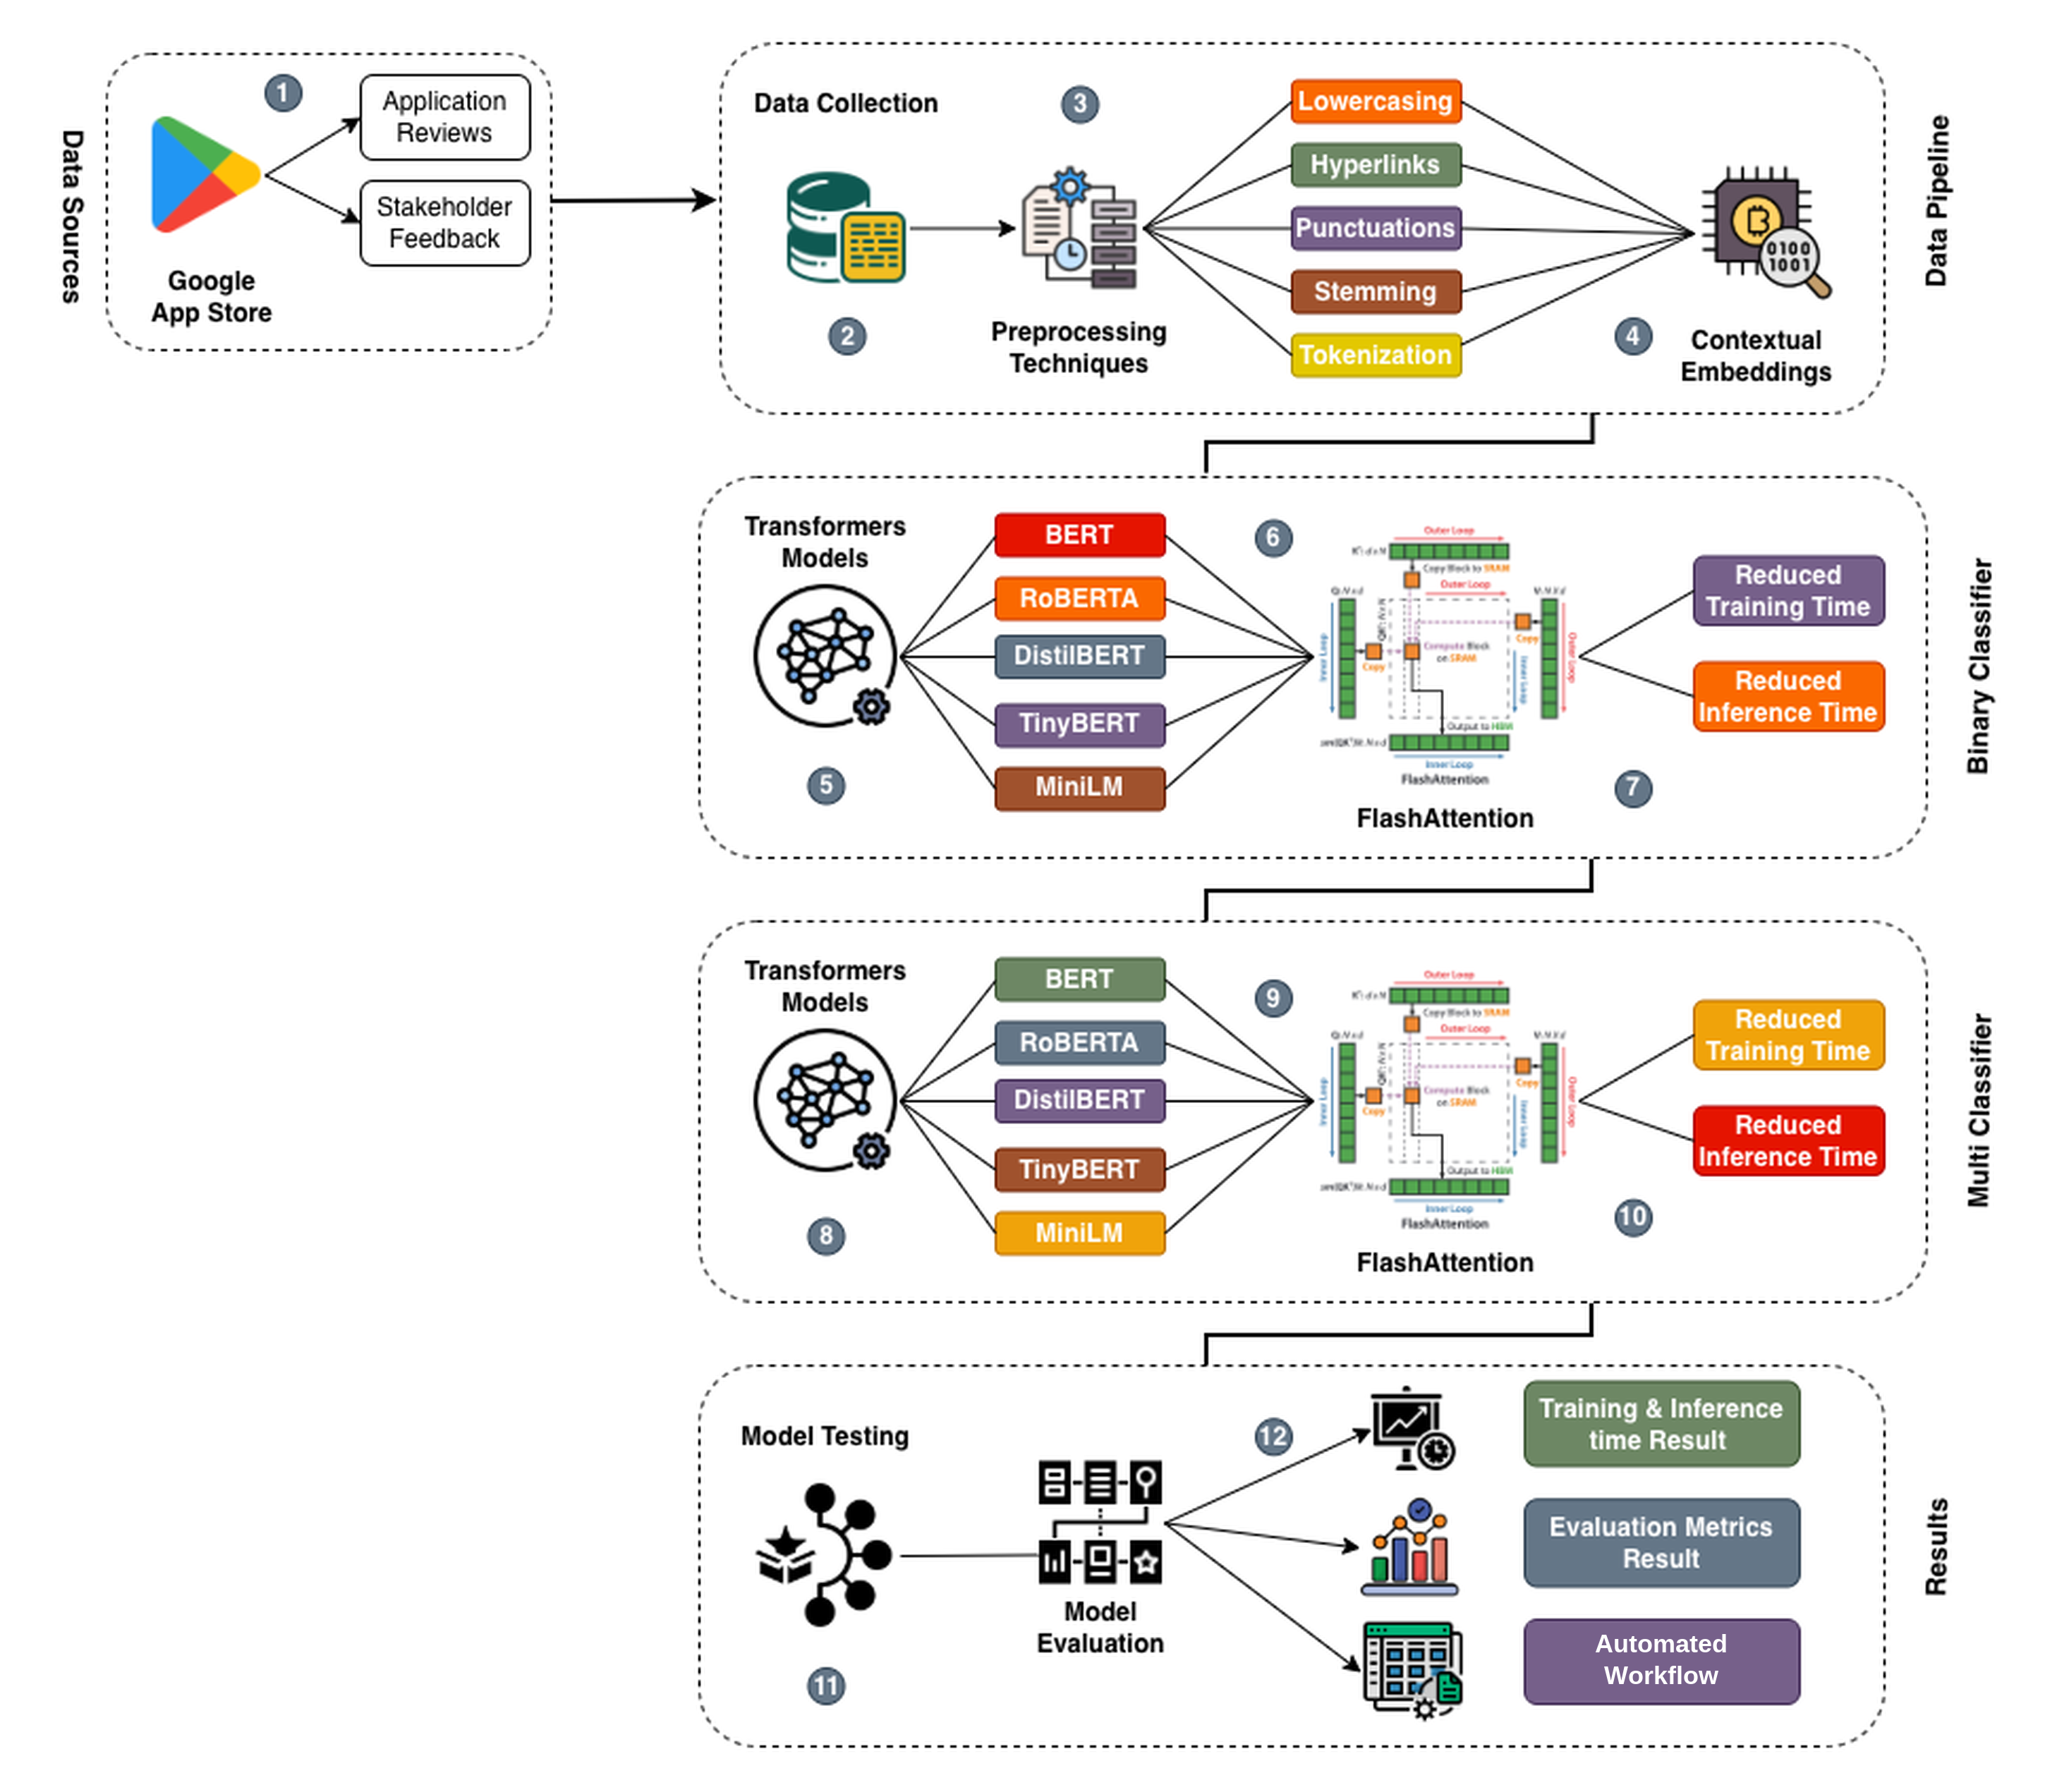
\includegraphics[width=0.92\textwidth]{fig1_framework.png}
\caption{End-to-End Sarcasm Identification Framework. \rcx{R5C5}{FlashAttention is drawn inside the two classification stages because it is the attention implementation used within each transformer encoder, and it is not a processing stage applied after classification.} \rcx{R5C1,R7C5}{The final box, which was previously labelled Agentic AI Automations, denotes the automated, confidence-aware workflow described in Section~\ref{sec:pipeline-method}.}}
\rcmark{R5C5}\rcmark{R5C1,R7C5}
\label{fig:framework}
\end{figure*}

As illustrated in \rcrep{R5C11}{(Figure 1)}{Figure~\ref{fig:framework}}, the framework is organized into five interconnected components. First, the \rce{\textit{Data Source}} stage gathers user reviews from the Google Play Store, providing a diverse and realistic dataset. Next, the \rce{\textit{Data Pipeline}} stage performs data collection, preprocessing, and contextual embedding, ensuring that raw textual inputs are transformed into structured representations suitable for modeling. The processed data is then passed to two parallel learning stages: \rce{\textit{Binary Classification}} and \rce{\textit{Multi-Class Classification}}. \rcrep{R5C5}{In both stages, transformer-based models are applied, and FlashAttention is incorporated to improve computational efficiency during training and inference.}{In both stages transformer encoders are fine-tuned, and FlashAttention is evaluated as the implementation of the attention computation inside each encoder, with the aim of reducing the cost of training and inference.} While the binary setting focuses on distinguishing sarcastic and non-sarcastic content, the multi-class setting captures fine-grained sarcasm types, enabling deeper understanding of user intent. Finally, the \rce{\textit{Results and Deployment}} stage evaluates model performance using standard metrics, analyzes training and inference efficiency, and \rcrep{R5C1,R7C5}{integrates the system into an agentic AI pipeline for continuous and automated operation}{integrates the selected model into an automated, confidence-aware orchestration pipeline for scheduled operation}.

To systematically explain how this framework operates, the following sections describe each component in detail. Specifically, we first formalize the problem setting, followed by dataset construction\rc{R5C9,R7C2}{, the audit of its annotations,} and preprocessing. We then explain how contextual representations are learned using transformer architectures, how classification is performed in both binary and multi-class settings, and how FlashAttention improves computational efficiency. Finally, we describe the \rcrep{R5C1,R7C5}{agentic AI pipeline}{automated, confidence-aware orchestration pipeline} and the end-to-end workflow integration, highlighting how all components interact to form a scalable and practical sarcasm detection system.

\subsection{Problem Formulation}
\label{sec:formulation}
\rcdel{R5C4}{Sarcasm detection is formulated as a supervised multi-class classification problem. Each review is represented as} \iftracked{\color{rvFive}\mbox{\rvstrikeplain{$r=\langle{T_r},{C_r}\rangle$.}}}\fi\ \rcdel{R5C4}{According to Equation (1), $T_r$ represents the textual content of the review, while $C_r$ denotes optional contextual information such as ratings or metadata. This formulation enables the model to incorporate both linguistic and contextual cues. The dataset is defined as $R=\{r_1,\ldots,r_n\}$ and the label space is formally defined in Equation (3) as $L=\{l_1,\ldots,l_k\}$.}
\begin{rcblock}{R5C4}
Sarcasm detection is formulated as two supervised classification tasks that share one formulation but use different datasets and label spaces. Each review is represented only by its text $T_r$, because the benchmark provides no ratings or other review metadata and no model in this study uses any input other than the review text. A dataset is therefore defined as
\end{rcblock}
\begin{equation}
\rcm{R5C4}{R = \{T_{1}, T_{2}, \ldots, T_{n}\},}
\label{eq:dataset}
\end{equation}
\rc{R5C4}{and the label spaces of the two tasks are}
\begin{equation}
\begin{gathered}
\rcm{R5C4}{L_{\mathrm{bin}} = \{\textit{Non-Sarcastic}, \textit{Sarcastic}\},} \\
\rcm{R5C4}{L_{\mathrm{type}} = \{\textit{Humor}, \textit{Irony}, \textit{Flattery}, \textit{Self-Deprecation}, \textit{Passive-Aggression}\}.}
\end{gathered}
\label{eq:labels}
\end{equation}
\rc{R5C4}{For either task, with $L \in \{L_{\mathrm{bin}}, L_{\mathrm{type}}\}$ and $k = |L|$,} the model learns a mapping
\begin{equation}
f : T_r \rightarrow P(L).
\label{eq:mapping}
\end{equation}
As defined in Equation~\eqref{eq:mapping}, the model outputs a probability distribution over \rcrep{R5C4}{sarcasm classes}{the classes of $L$}. During training, the objective is formulated using cross-entropy loss\rce{:}
\begin{equation}
\mathcal{L}(\theta) = -\sum_{i=1}^{n}\sum_{j=1}^{k} y_{ij}\,\log f_{j}(T_{r_i};\theta).
\label{eq:loss}
\end{equation}
As described in Equation~\eqref{eq:loss}, the model minimizes the difference between predicted probabilities and true labels. During inference, the predicted label is selected as
\begin{equation}
l^{*} = \arg\max_{l \in L} f_{l}(T_r;\theta).
\label{eq:argmax}
\end{equation}
This mathematical formulation provides the foundation for the entire pipeline, guiding both training and prediction processes\rcdel{R7C7}{in above Equation (6)}.

\subsection{Dataset Description}
\label{sec:dataset}
For this study, we employed a publicly available benchmark dataset\footnote{The dataset was originally introduced by \citet{fatima2024exploratory} for sarcasm identification in mobile app reviews and provides a manually annotated corpus designed for fine-grained sarcasm classification.} \rcrep{R7C7}{consisting of}{built from} approximately 55,000 user reviews collected from the Google Play Store using the official Google Play Scraper API.\footnote{Google Play Scraper API: \url{https://pypi.org/project/google-play-scraper/}.} The dataset reflects realistic and large-scale user feedback generated within mobile software ecosystems, making it suitable for evaluating sarcasm-aware sentiment analysis in Natural Language-Based Software Engineering (NLbSE) environments. The corpus includes reviews from seven widely used social and entertainment applications: TikTok, Instagram, Akinator, iDrink, Make It Rain, One Star App: Lowest Rated App, and Nothing. These applications were \rcrep{R7C7}{intentionally selected}{selected by the original authors} because they contain highly interactive user communities where expressive, emotional, humorous, and sarcastic communication patterns frequently occur. As a result, the dataset captures diverse linguistic behaviors, including implicit criticism, exaggerated praise, irony, humor, and passive-aggressive feedback that commonly appear in real-world app reviews.

The annotated corpus supports two distinct and separately evaluated classification tasks, and this manuscript reports them separately throughout. The binary task is defined over the full annotated corpus and distinguishes sarcastic from non-sarcastic reviews. The sarcasm-type task is defined \rcrep{R5C9,R7C2}{only over the subset of reviews that were annotated as sarcastic, and classifies them}{over a separately released file of reviews annotated with a sarcasm type, and classifies them} into the five sarcasm categories Humor, Irony, Flattery, Self-Deprecation, and Passive-Aggression. The two tasks use different label spaces and different numbers of instances, they were never merged into a single six-class problem, and no result reported in this manuscript combines them. The scraped collection contains approximately 55,000 reviews from seven mobile applications, of which the original authors manually annotated a stratified sample of 10,000 reviews. The distinction between the scraped collection and the annotated corpus matters for the interpretation of every result in this manuscript, because all supervised training and evaluation reported here use only the annotated corpus. The binary dataset used in this study contains 9,999 usable annotated reviews, of which 6,539 are non-sarcastic and 3,460 are sarcastic, corresponding to a sarcasm rate of 34.6\%. \rcrep{R5C9,R7C2}{The sarcasm-type dataset contains the 3,460 sarcastic reviews.}{The sarcasm-type dataset contains 3,460 reviews, which is the same number as the sarcastic reviews of the binary file and which led the previous version of this manuscript to describe it as the set of those sarcastic reviews. Matching the two files on normalized text shows, however, that it is not a strict subset of them, since 3,101 of its reviews correspond to reviews labelled sarcastic in the binary file, 253 correspond to reviews labelled non-sarcastic there, and 106 have no counterpart in the binary file. The sarcasm-type file is therefore a separately released annotation, which affects no reported metric because the two tasks are trained and evaluated independently, but which matters for a cascaded deployment in which the type classifier is applied only to reviews that the binary classifier flags, as discussed in Section~\ref{sec:threats}.} \rcrep{R5C11}{Tables 2 and 3}{Tables~\ref{tab:apps} and~\ref{tab:composition}} summarize the distribution of the scraped collection across source applications and the composition of the two annotated task datasets, respectively.

\begin{table}[t]
\caption{Distribution of Reviews Across Source Applications}
\label{tab:apps}
\centering\small
\begin{tabular}{lrr}
\toprule
Source Application & Reviews & Percentage \\
\midrule
Akinator & 12,000 & 21.8\% \\
TikTok & 10,000 & 18.2\% \\
Make It Rain & 9,000 & 16.4\% \\
One Star App & 8,000 & 14.5\% \\
iDrink & 6,000 & 10.9\% \\
Instagram & 5,000 & 9.1\% \\
Nothing & 5,000 & 9.1\% \\
\midrule
Total & 55,000 & 100.0\% \\
\bottomrule
\end{tabular}
\end{table}

\begin{table}[t]
\caption{Composition of the two annotated task datasets. Percentages for the sarcasm-type dataset are relative to \rcrep{R5C9,R7C2}{the 3,460 sarcastic reviews}{its 3,460 reviews}.}
\rcmark{R5C9,R7C2}
\label{tab:composition}
\centering\small
\begin{tabular}{lrr}
\toprule
Category & Reviews & Percentage \\
\midrule
\multicolumn{3}{l}{\textit{Binary task dataset (9,999 annotated reviews)}} \\
Non-Sarcastic & 6,539 & 65.4\% \\
Sarcastic & 3,460 & 34.6\% \\
\midrule
\multicolumn{3}{l}{\textit{Sarcasm-type task dataset (3,460 \rcdel{R5C9,R7C2}{sarcastic} reviews)}} \\
Humor & 1,709 & 49.4\% \\
Irony & 536 & 15.5\% \\
Flattery & 513 & 14.8\% \\
Self-Deprecation & 439 & 12.7\% \\
Passive-Aggression & 263 & 7.6\% \\
\bottomrule
\end{tabular}
\end{table}

This fine-grained labeling structure enables the evaluation of nuanced contextual and pragmatic differences between multiple forms of sarcastic expression, rather than limiting the analysis to binary sarcasm detection. However, although the dataset includes several important sarcasm categories, it does not explicitly represent other linguistically recognized forms such as hyperbolic sarcasm, rhetorical sarcasm, dropped-negation sarcasm, oxymoronic sarcasm, and deadpan sarcasm. Consequently, the proposed framework is primarily optimized for the sarcasm patterns represented within the annotated corpus. Nevertheless, the framework remains extensible and can be adapted to incorporate additional sarcasm categories through expanded annotation schemes, discourse-aware contextual modeling, conversational context integration, and domain-adaptive fine-tuning strategies in future work. The class distribution shown in \rcrep{R5C11}{Table 3}{Table~\ref{tab:composition}} indicates a naturally imbalanced benchmark, with non-sarcastic reviews accounting for 65.4\% of the annotated corpus, whereas several sarcasm categories, \rcrep{R5C8,R7C1}{particularly Self-Deprecation (2.6\%), Passive Aggression (4.4\%), and Flattery (5.1\%), contain substantially fewer training instances}{particularly Passive-Aggression (7.6\% of the sarcasm-type dataset), Self-Deprecation (12.7\%) and Flattery (14.8\%), contain substantially fewer instances than Humor (49.4\%)}. Such imbalance is expected in naturally occurring user-generated content because certain forms of sarcasm appear considerably less frequently than others. Class imbalance may bias deep learning models toward majority classes, potentially reducing recall for minority sarcasm categories. To mitigate this issue during model development, the training data were balanced using RandomOverSampler prior to model training, while the held-out evaluation set retained the original benchmark distribution. Furthermore, Macro F1-score was reported alongside Weighted F1-score to ensure that performance on minority sarcasm categories was evaluated fairly rather than being dominated by the majority class.

\rcdel{R5C8,R7C1}{One inconsistency in the label mapping should be reported explicitly rather than corrected silently. In the source publication that introduced this benchmark, the category Passive Aggression is reported with 439 instances and Self-Deprecation with 263 instances. In the label mapping used by the result files of the present study, the counts are associated with the categories in the opposite order, so that Self-Deprecation carries 439 instances and Passive-Aggression carries 263 instances. The class supports observed in the held-out test partitions, namely 65 and 40 instances respectively, are consistent with the mapping used in our result files. We have therefore reported the class names exactly as they appear in the experimental output rather than reassigning them, and we note that readers comparing the per-class results in Section 6 against the source publication should account for this discrepancy. Resolving which of the two mappings reflects the original annotation requires access to the original annotation records and is identified as an open item.}

\paragraph{\rcx{R5C8,R7C1}{Resolution of the category names}}
\begin{rcblock}{R5C8,R7C1}
The source publication that introduced this benchmark reports 439 instances for Passive Aggression and 263 for Self-Deprecation, whereas the files used here associate these counts with the two categories in the opposite order. We resolved this discrepancy against the released data instead of leaving it open, and three independent observations support the names used in this study. First, both released files store the categories as text strings rather than as integer codes, and the experiments read these strings directly, so there is no mapping step at which the two names could have been exchanged; in the sarcasm-type file the category with 439 reviews carries the string \textit{Self-Deprecation} and the category with 263 reviews carries the string \textit{Passive-Aggression}. Second, the binary file contains its own sarcasm-type column, annotated independently of the sarcasm-type file, and 427 of the 439 reviews of the first category are named \textit{Self-Deprecation} in that column as well. Third, the content of the two categories agrees with the released names. In a random sample of 30 reviews from each category, the reviews labelled \textit{Passive-Aggression} are veiled complaints addressed to the developer, for example ironic praise of the effort spent on fake reviews or polite requests to reduce advertisements, and 18.3\% of all reviews in this category address the developer or request a fix, which is the highest share of any category. The reviews labelled \textit{Self-Deprecation} consist mainly of exaggerated mock condemnation that echoes the self-deprecating premise of applications such as One Star App, and 85.4\% of them contain the word ``worst''. Exchanging the two names would therefore assign developer-directed complaints to self-deprecation, which neither annotation supports. We retain the names of the released benchmark and attribute the discrepancy to the count table of the source publication, so readers who compare our per-class results with that publication should read its Passive Aggression count as corresponding to the Self-Deprecation category of the released data. The sample and the counts are provided as supplementary material, and Section~\ref{sec:threats} notes that in this benchmark the Self-Deprecation category denotes mock self-condemnation by or about the application rather than the narrower linguistic sense of a speaker who mocks themselves.
\end{rcblock}

Following the original benchmark dataset construction, the annotation process was independently performed by three annotators, including one MS student, one PhD student, and one senior faculty member. The annotation quality achieved an average inter-annotator agreement of 88\%, corresponding to a Cohen's $\kappa$ coefficient of 0.68, indicating substantial agreement among the annotators. Reviews with conflicting annotations were subsequently discussed until consensus was reached\rcrep{R5C9,R7C2}{, resulting in a conflict-free benchmark dataset}{, although the released files nevertheless contain the conflicting labels documented in Section~\ref{sec:duplicates}}. The annotation guidelines were adapted from established sarcasm detection literature \citep{fatima2024exploratory,sinha2023sarcasm,eke2020sarcasm}, with particular emphasis on contextual polarity, implicit sentiment contradiction, and communicative intent \citep{kamal2022cat,eke2020sarcasm}.

The dataset is particularly suitable for evaluating transformer-based and inference-optimized sarcasm detection frameworks because it combines informal language, emotionally expressive content, software-specific terminology, and long contextual reviews within a realistic software feedback environment. These characteristics make sarcasm identification substantially more challenging than traditional sentiment analysis tasks and provide a useful benchmark \rcdel{R7C7}{for evaluating} for assessing both classification effectiveness and real-world deployment scalability.

\subsubsection{\texorpdfstring{\rcx{R5C9,R7C2}{Duplicated and Conflicting Annotations}}{Duplicated and Conflicting Annotations}}
\label{sec:duplicates}
\begin{rcblock}{R5C9,R7C2}
Both released files contain repeated reviews. To identify them, we matched reviews on a normalized key in which letter case and whitespace are collapsed and non-ASCII bytes are removed, so that copies of the same review that differ only in spacing, capitalization or mis-encoded characters are recognized as the same text. This matching is stricter than the exact string comparison used in the previous version, which found 82 and 487 rows belonging to duplicated groups in the binary and sarcasm-type files respectively, and Table~\ref{tab:dedup-audit} summarizes its result. In the binary file, 73 rows repeat an earlier review and every repeated review carries the same label. In the sarcasm-type file, 289 rows repeat an earlier review, and 230 texts covering 461 rows appear with two or more different sarcasm types, the most frequent pairs being Humor with Self-Deprecation (73 texts), Irony with Self-Deprecation (48 texts) and Humor with Irony (42 texts). These texts are in effect multi-label annotations stored as separate single-label rows, and a single-label classifier cannot predict both labels of such a text.

The duplicates affect the released-benchmark partitions in two different ways. In the binary task, between 13 and 14 test reviews per seed also occur in the training partition, always with the same label; such pairs could inflate the test scores, but they amount to less than 1\% of the 1,500 test reviews and therefore cannot change accuracy by more than that amount. In the sarcasm-type task, between 60 and 66 test reviews per seed also occur in the training partition, yet only 9 to 15 of them occur there with the same label, while 45 to 52 occur in training only under a different label. These conflicting pairs cannot inflate the scores and, if anything, lower them, because the model is trained towards a label that differs from the one on which it is tested. To remove both effects, we additionally evaluate a deduplicated protocol (Section~\ref{sec:protocols}), in which every text that carries conflicting labels is removed and every repeated text with a consistent label is kept once before the partitions are drawn. The deduplicated binary dataset contains 9,926 reviews (6,475 non-sarcastic and 3,451 sarcastic), and the deduplicated sarcasm-type dataset contains 2,941 reviews (1,555 Humor, 489 Flattery, 385 Irony, 297 Self-Deprecation and 215 Passive-Aggression).
\end{rcblock}

\begin{table}[t]
\caption{\rcx{R5C9,R7C2}{Audit of repeated and conflicting annotations in the released benchmark files, using normalized text matching.}}
\rcmark{R5C9,R7C2}
\label{tab:dedup-audit}
\centering\small
\iftracked\color{rvBoth}\fi
\begin{adjustbox}{max width=\textwidth}
\begin{tabular}{lrr}
\toprule
 & Binary file & Sarcasm-type file \\
\midrule
Rows & 9,999 & 3,460 \\
Distinct texts & 9,926 & 3,171 \\
Rows repeating an earlier text & 73 & 289 \\
Texts with conflicting labels (rows) & 0 (0) & 230 (461) \\
Retained after deduplication & 9,926 & 2,941 \\
\midrule
Test reviews also in training, per seed (released partitions) & 13 to 14 & 60 to 66 \\
\quad of which with the same label in training & 13 to 14 & 9 to 15 \\
\bottomrule
\end{tabular}
\end{adjustbox}
\end{table}

\subsubsection{Data Preprocessing}
The preprocessing stage converts raw reviews into structured inputs suitable for Transformer Language Models. This stage removes noise such as URLs and irrelevant symbols, applies normalization (lowercasing and contraction expansion), and converts emojis into textual tokens. Each processed review is tokenized using model-specific tokenizers and transformed into a fixed-length sequence of 128 tokens through padding and truncation. This ensures uniform input representation across the dataset. The output of this stage serves as the direct input to the contextual embedding module, ensuring that the model receives clean yet expressive data that preserves sarcasm-related cues.

\subsection{Contextual Representation}
Sarcasm is inherently context-dependent \citep{ibitoye2025contextual}, often arising from contradictions between different parts of a sentence. To capture such relationships, the proposed framework employs transformer-based models with self-attention mechanisms \citep{wang2025spatial}. Formally, given an input sequence $X = \{x_1, x_2, \ldots, x_n\}$, the contextual representation of each token is computed using the self-attention mechanism
\begin{equation}
\mathrm{Attention}(Q,K,V) = \mathrm{softmax}\!\left(\frac{QK^{\top}}{\sqrt{d_k}}\right)V.
\label{eq:attention}
\end{equation}
According to Equation~\eqref{eq:attention}, the matrices $Q$, $K$, and $V$ are linear projections of the input embeddings. This formulation allows each token to attend to all other tokens in the sequence, capturing long-range dependencies. To enhance representation learning, multi-head attention is applied:
\begin{equation}
\mathrm{MultiHead}(Q,K,V) = \mathrm{Concat}(\mathrm{head}_1,\ldots,\mathrm{head}_h)W^{O},
\label{eq:multihead}
\end{equation}
where each head is defined as
\begin{equation}
\mathrm{head}_i = \mathrm{Attention}(QW_i^{Q}, KW_i^{K}, VW_i^{V}).
\label{eq:head}
\end{equation}
This mechanism enables the model to capture multiple semantic relationships simultaneously, which is critical for identifying subtle forms of sarcasm.

\subsection{Classification Learning}
The contextual embedding generated by the transformer is used to perform sarcasm classification. Let $h_i \in \mathbb{R}^{d}$ denote the embedding of the input sequence, typically corresponding to the [CLS] token. The classification probability is computed as
\begin{equation}
p(y \mid h_i) = \mathrm{softmax}(W h_i + b).
\label{eq:classifier}
\end{equation}
According to Equation~\eqref{eq:classifier}, $W \in \mathbb{R}^{k\times d}$ and $b \in \mathbb{R}^{k}$ are learnable parameters, and $k$ represents the number of \rcrep{R5C4}{sarcasm classes}{classes of the task}. The training objective minimizes the cross-entropy loss
\begin{equation}
\mathcal{L}(\theta) = -\sum_{i=1}^{n}\sum_{j=1}^{k} y_{ij}\,\log p_j(y \mid h_i).
\label{eq:cls-loss}
\end{equation}
This optimization ensures that the predicted distribution aligns with the true labels. To improve generalization, dropout is applied:
\begin{equation}
\tilde{h}_i = \mathrm{Dropout}(h_i).
\label{eq:dropout}
\end{equation}
This reduces overfitting by preventing co-adaptation of features. \rcrep{R5C5}{The classification output produced in this stage is then forwarded to the efficiency optimization layer, ensuring that both accuracy and computational performance are maintained.}{The predicted distribution of Equation~\eqref{eq:classifier} is the output of the classification stage and is passed to the confidence-based routing stage of Section~\ref{sec:pipeline-method}. FlashAttention does not act on this output, because it changes only how the attention of Equation~\eqref{eq:attention} is computed inside the encoder that produces $h_i$, as described in Section~\ref{sec:fa-method}.}

\subsection{FlashAttention Optimization}
\label{sec:fa-method}
The standard attention mechanism has quadratic complexity
\begin{equation}
\mathcal{O}(n^{2}d),
\label{eq:complexity}
\end{equation}
which becomes a bottleneck for long input sequences.\rcdel{R7C7}{As defined earlier in Equation (13), this limits scalability.} To address this, FlashAttention \citep{dao2022flashattention,dao2024flashattention2} restructures the computation into memory-efficient blocks\rcrep{R7C7}{: FlashAttention partitions}{. It partitions} $Q$, $K$, and $V$ into blocks that fit in on-chip memory and accumulates the attention output block by block using an online softmax formulation. Crucially, the partial results are not normalized independently. Instead, a running maximum $m$ and a running normalization constant $\ell$ are maintained across blocks, and the accumulated output is rescaled whenever a new block updates the running maximum. For the $j$-th key block, let
\begin{equation}
S_j = \frac{QK_j^{\top}}{\sqrt{d_k}}, \qquad m^{(j)} = \max\!\left(m^{(j-1)}, \max S_j\right).
\label{eq:fa-scores}
\end{equation}
The running normalizer and the accumulated output are then updated as
\begin{equation}
\ell^{(j)} = e^{m^{(j-1)}-m^{(j)}}\,\ell^{(j-1)} + \sum \exp\!\left(S_j - m^{(j)}\right),
\label{eq:fa-norm}
\end{equation}
\begin{equation}
O^{(j)} = e^{m^{(j-1)}-m^{(j)}}\,O^{(j-1)} + \exp\!\left(S_j - m^{(j)}\right)V_j,
\label{eq:fa-out}
\end{equation}
and the final attention output is recovered as $O = O^{(B)}/\ell^{(B)}$ after the last block. Because the rescaling factors restore the global normalization at every step, Equations~\eqref{eq:fa-scores} \rce{to}~\eqref{eq:fa-out} compute the same values as the global softmax attention of Equation~\eqref{eq:attention} up to floating-point rounding. FlashAttention therefore changes the order and locality of the computation rather than the function that is computed, and it is not an approximation of attention by a collection of independently normalized blocks. \rcrep{R5C12}{Additionally, FlashAttention optimizes Wang et al. (2020) memory access by minimizing reads and writes, so that the memory cost becomes}{In addition, FlashAttention reduces reads from and writes to high-bandwidth memory \citep{dao2022flashattention}, so that the additional memory required by attention grows as}
\begin{equation}
\mathcal{O}(nd)
\label{eq:fa-memory}
\end{equation}
\rc{R5C12}{rather than with the full $n \times n$ attention matrix.} \rcdel{R7C4}{This leads to significant improvements in GPU utilization and training speed.} Unlike approximate attention methods, FlashAttention preserves exact attention values, so the semantic relationships captured during contextual modelling remain intact. This property is important for sarcasm detection, where subtle contextual cues must not be lost.

Because FlashAttention operates at the level of the attention computation inside the transformer encoder, it must be understood as a property of the encoder stage rather than as a post-classification transformation. The end-to-end formulation in \rcrep{R5C11}{Section 3.8}{Section~\ref{sec:workflow}} reflects this placement. It is also necessary to distinguish four related notions that are sometimes used interchangeably. Standard attention refers to the mathematical definition in Equation~\eqref{eq:attention}. Eager attention refers to the reference implementation that materializes the full attention matrix in high-bandwidth memory and is the baseline condition in our experiments. Scaled dot-product attention refers to the fused PyTorch operator that may dispatch to one of several backends. FlashAttention refers to the specific input-output-aware kernel evaluated here. In every experiment reported as a FlashAttention condition in \rcrep{R5C11}{Section 6.1}{Section~\ref{sec:efficiency}}, the active backend was verified programmatically at runtime before training, and only runs for which a forward pass completed under a FlashAttention-only backend were retained. Results obtained under eager attention are reported as such and are never labelled as FlashAttention results. The empirical evaluation in \rcrep{R5C11}{Section 6.1}{Section~\ref{sec:efficiency}} reports training time, inference latency, and peak allocated GPU \rcrep{R7C4}{memory for both training and inference}{training memory}.

\subsection{Automated Confidence-Aware Pipeline}
\label{sec:pipeline-method}
The final stage of the framework integrates the trained model into an automated pipeline \rcrep{R5C1,R7C5}{capable of continuous operation}{for scheduled operation}. Rather than operating as a static classifier, the system evaluates the confidence of every prediction and determines on that basis whether the prediction is accepted directly or routed for additional processing. This confidence-conditioned branch is the only decision point in the pipeline. The pipeline is therefore best described as automated workflow orchestration with confidence-based routing, and it does not exhibit planning, goal generation, or tool selection. The proposed pipeline follows \rcrep{R7C7}{an event-driven workflow designed to support recurring software feedback analysis..}{a scheduled workflow designed to support recurring software feedback analysis.} Newly submitted Google Play reviews are periodically retrieved and forwarded to the preprocessing module, where text normalization and tokenization are performed before transformer inference. The selected Transformer Language Model generates both the predicted sarcasm category and its associated confidence score. Predictions with confidence scores greater than or equal to the predefined threshold ($\tau = 0.7$) are accepted automatically and stored within the cloud-based analytics repository for downstream visualization and reporting. Conversely, predictions with confidence scores below the threshold are routed to a secondary processing stage, which re-evaluates the review using the same trained Transformer Language Model and flags the outcome for optional human review. Because this stage uses the same model rather than an independent verifier, it is described throughout as confidence-based routing rather than as verification. The routed prediction is subsequently stored together with its confidence score and processing metadata. Given an input review $T_r$, the primary prediction is computed as
\begin{equation}
l^{*} = \arg\max_{l \in L} f_{l}(T_r;\theta).
\label{eq:primary}
\end{equation}
To support confidence-based routing, the model confidence is evaluated against a predefined threshold. Let
\begin{equation}
c = \max_{l} f_{l}(T_r;\theta).
\label{eq:confidence}
\end{equation}
If $c < \tau$, the review is routed to the secondary processing stage $g(\cdot)$, which applies the same fine-tuned model:
\begin{equation}
\rcm{R5C7}{l_{\mathrm{route}}} = g(T_r).
\label{eq:secondary}
\end{equation}
The final decision is determined as
\begin{equation}
l_{\mathrm{final}} =
\begin{cases}
l^{*}, & \text{if } c \geq \tau,\\
\rcm{R5C7}{l_{\mathrm{route}}}, & \text{otherwise.}
\end{cases}
\label{eq:final}
\end{equation}
\rcnote{R5C7}{In Equations (20) and (21) the symbol $l_{\mathrm{route}}$ replaces $l_{\mathrm{verify}}$ of the previous version, because the secondary stage re-applies the same model and does not verify the prediction.}

Following prediction, aggregated sarcasm statistics, category distributions, and temporal trends are automatically synchronized with the cloud analytics layer\rc{R5C1,R7C5}{ at the cadence of the scheduled ingestion}, allowing software engineers and application developers to monitor evolving user feedback\rcdel{R5C1,R7C5}{in near real time}. This deployment-oriented orchestration separates prediction, \rcrep{R5C7}{verification}{routing}, storage, and visualization into independent processing stages, enabling scalable execution while minimizing computational overhead. Model maintenance is performed independently from the online inference workflow. Rather than continuously retraining the Transformer Language Model after every incoming review, newly collected reviews are accumulated over time and incorporated into scheduled offline retraining cycles when sufficient additional labeled data become available. This design avoids unnecessary computational cost while maintaining deployment stability and allowing the framework to adapt to evolving sarcasm patterns through periodic model updates. Separating online inference from offline retraining also reduces system downtime and improves reproducibility because every deployed model version is trained using a fixed dataset and experimental configuration.

This two-stage mechanism concentrates additional computation on the predictions about which the model is least certain, which is desirable in a \rcrep{R5C1,R7C5}{continuously operating pipeline}{pipeline that runs repeatedly} because it bounds the additional cost while surfacing uncertain cases for human attention. For all experiments reported in this manuscript the confidence threshold was fixed at $\tau = 0.7$. The limitations of this mechanism should be stated plainly. Because the routed predictions are re-evaluated by the same deterministic model on the same input, the routing stage does not by itself change any prediction and therefore cannot improve accuracy. Its function is triage rather than correction, and the choice of threshold governs computational cost and the volume of flagged cases rather than predictive performance. A routing stage that is capable of correcting predictions would require an independent model, an alternative input view, or an ensemble decision, \rcrep{R7C3}{and the design and empirical evaluation of such a stage remain future work.}{and Section~\ref{sec:routing} evaluates such a stage built from the other fine-tuned encoders.} We further note that the threshold sensitivity analysis reported in the previous version of this manuscript was computed on an evaluation partition that does not correspond to the test partitions used in the present experimental protocol, and it has therefore been withdrawn rather than restated. \rcrep{R7C3}{This is recorded as an open item in Section 8.}{It is replaced by a new analysis on the deduplicated test partitions in Section~\ref{sec:routing}, which tests the two properties on which the usefulness of this triage depends, namely whether the confidence score is calibrated and whether predictions below the threshold are in fact less accurate than those above it. Temperature scaling \citep{guo2017calibration}, fitted on the validation partition, can be applied to the confidence score before thresholding without changing any predicted label, because it preserves the arg max of the distribution, and the same section tests whether it improves calibration.} The pipeline interacts with external systems on a scheduled basis, retrieving new reviews, processing them and updating results. This extends the model from a static classifier into an automated processing component that supports low-latency analysis of incoming feedback \rce{\citep{sharma2026toward}}.

\subsection{End-to-End Workflow Integration}
\label{sec:workflow}
The proposed framework operates as a tightly integrated pipeline where each stage contributes to the final outcome. Formally, the complete process can be expressed as a composition of functions:
\begin{equation}
\rcm{R5C6}{l_{\mathrm{final}} = \Phi_{\mathrm{route}} \circ \Phi_{\mathrm{cls}} \circ \Phi_{\mathrm{enc}}^{(a)} \circ \Phi_{\mathrm{prep}}(T_r), \qquad a \in \{\text{eager}, \text{FlashAttention}\},}
\label{eq:composition}
\end{equation}
\rcnote{R5C6}{The previous version of Equation (22) read $l_{\mathrm{final}}=\Phi_{\mathrm{agent}}\circ\Phi_{\mathrm{flash}}\circ\Phi_{\mathrm{cls}}\circ\Phi_{\mathrm{enc}}\circ\Phi_{\mathrm{prep}}(T_r)$, which placed FlashAttention after classification.}
where:
\begin{itemize}
\item $\Phi_{\mathrm{prep}}$ represents preprocessing,
\item \rcrep{R5C6}{$\Phi_{\mathrm{enc}}$ denotes contextual encoding,}{$\Phi_{\mathrm{enc}}^{(a)}$ denotes contextual encoding, in which every attention layer computes Equation~\eqref{eq:attention} with implementation $a$; with $a = \text{FlashAttention}$ the computation follows Equations~\eqref{eq:fa-scores} to~\eqref{eq:fa-out}, so the efficiency optimization is part of the encoder rather than a separate stage,}
\item $\Phi_{\mathrm{cls}}$ corresponds to classification,
\item \rcdel{R5C6}{$\Phi_{\mathrm{flash}}$ applies efficiency optimization,}
\item \rcrep{R5C6}{$\Phi_{\mathrm{agent}}$}{$\Phi_{\mathrm{route}}$} represents confidence-based routing and workflow orchestration.
\end{itemize}
\rcrep{R5C6}{According to Equation (22), the system processes raw input through a sequence of transformations, each enhancing the representation and reliability of predictions.}{Because $\Phi_{\mathrm{enc}}^{(\text{eager})}$ and $\Phi_{\mathrm{enc}}^{(\text{FlashAttention})}$ compute the same function up to floating-point rounding, the choice of $a$ affects the cost of the pipeline rather than its predictions.} This integrated design ensures that the framework remains scalable, efficient, and deployable in realistic environments. The automation properties of the framework arise from its ability to coordinate prediction, confidence evaluation, routing, and cloud-based reporting without manual intervention at run time. These capabilities transform the framework from a conventional prediction model into an operational software analytics component, and they do so through predefined orchestration rather than through autonomous decision-making.

\subsection{Algorithmic Description}
The complete workflow of the proposed framework is described in Algorithm~\rcrep{R5C11}{3.9}{\ref{alg:workflow}}. The algorithm integrates data \rcrep{R5C9,R7C2}{collection}{preparation}, preprocessing, training, prediction, confidence-based routing, and automated deployment.

\begin{algorithm}[t]
\caption{Transformer-Based Sarcasm Detection and Automated Deployment}
\label{alg:workflow}
\begin{algorithmic}[1]
\Require \rcrep{R5C4}{Raw reviews $R=\{r_1,\ldots,r_n\}$}{Annotated reviews $R = \{T_1,\ldots,T_n\}$}; Transformer Language Models $C$; \rc{R5C6}{attention implementation $a \in \{\text{eager}, \text{FlashAttention}\}$;} threshold ($\tau = 0.7$)
\Ensure Best model $m^{*}$ and deployed automated pipeline
\State \textbf{Data \rcrep{R5C9,R7C2}{Collection}{Preparation}:} \rcrep{R5C9,R7C2}{Scrape reviews and label them into sarcasm categories}{load the annotated benchmark, optionally remove conflicting and repeated texts (Section~\ref{sec:duplicates}), and draw stratified partitions}
\State \textbf{Preprocessing:} Clean and tokenize each review using the standardized pipeline
\State \textbf{Training Phase}
\For{each model $m \in C$}
  \State \rcrep{R5C6}{Train $m$ using FlashAttention}{Fine-tune $m$ with attention implementation $a$ on the oversampled training partition}
  \State Optimize parameters via cross-entropy loss
\EndFor
\State \textbf{Model Selection}
\State Choose $m^{*}$ with highest validation \rce{Macro} F1-score
\State \textbf{Automated Deployment}
\While{new reviews are available}
  \State Fetch new rows using \texttt{tool\_fetch\_unlabeled()}
  \State Preprocess text
  \State Predict sarcasm label $l^{*}$ \rc{R7C7}{and its confidence $c$}
  \If{\rcrep{R7C7}{$f_{l^{*}}<\tau$}{$c < \tau$}}
    \State Route to secondary processing stage \rc{R5C7}{and flag for review}
  \EndIf
  \State Write prediction to Google Sheets
\EndWhile
\State \Return $m^{*}$
\end{algorithmic}
\end{algorithm}

The proposed approach integrates fine-tuned Transformer Language Models, FlashAttention acceleration, and \rcrep{R5C1,R7C5}{a continuously operating automated pipeline}{an automated pipeline that runs on a schedule}. The resulting system reads user feedback, classifies it, routes uncertain predictions for additional processing, and writes structured labels back to a cloud analytics layer, which turns sarcasm detection from a research experiment into a practical component for software teams.

%% ============================================================================
\section{Illustrative Deployment Example}
\label{sec:example}

\begin{examplebox}{End-to-End Sarcasm Detection with \rcrep{R5C1,R7C5}{Agentic Pipeline}{the Automated Confidence-Aware Pipeline}}
\textbf{Input App Review:} ``Great update! Now the app crashes even faster than before.''

\medskip\textbf{Step 1: Data Ingestion (Data Source).} The review is automatically collected from the Google Play Store and passed into the system as input $T_r$ (Equation~\eqref{eq:dataset}).

\medskip\textbf{Step 2: Preprocessing (Data Pipeline).} The raw text is cleaned and normalized: \textit{great update now app crashes faster than before}. This ensures that noise is removed while preserving sarcasm-related cues.

\medskip\textbf{Step 3: Contextual Representation.} The processed text is encoded using a Transformer Language Model. According to Equation~\eqref{eq:attention}, self-attention captures relationships between all tokens. \rcrep{R7C6}{Strong attention is observed between ``great update'' (positive cue) and ``crashes faster'' (negative outcome), and this contradiction forms the core sarcasm signal.}{In this example the sarcasm signal is the contrast between the positive cue ``great update'' and the negative outcome ``crashes faster''; we did not analyse attention weights, so this step describes the cue that the model must resolve rather than an observed attention pattern.}

\medskip\textbf{Step 4: Classification (Binary + Multi-Class).} The contextual embedding $h_i$ is passed to the classifier $p(y\mid h_i) = \mathrm{softmax}(Wh_i+b)$. The model assigns probabilities:
\begin{itemize}
\item Binary: \textit{Sarcastic} (high)
\item Multi-class: \textit{Irony} (highest probability)
\end{itemize}
Prediction is obtained using Equation~\eqref{eq:argmax}.

\medskip\textbf{Step 5: Efficiency Optimization (FlashAttention).} During inference, \rc{R5C5}{inside the encoder used in Steps 3 and 4,} FlashAttention (Equation~\eqref{eq:fa-out}) optimizes the attention computation by reducing memory movement. In the experiments reported in \rcrep{R5C11}{Section 6.1}{Section~\ref{sec:efficiency}} this lowers inference latency, which supports low-latency processing of incoming app-review streams. The computation performed is unchanged, so no effect on the predicted label is expected from this step.

\medskip\textbf{Step 6: Confidence Evaluation and Routing.} The confidence score $c = \max_l f_l(T_r)$ is computed. If $c < \tau$, the \rcrep{R5C7}{verification model (Equation (20)) is triggered}{review is passed to the secondary processing stage (Equation~\eqref{eq:secondary}) and flagged for review}; otherwise, the prediction is accepted. This confidence-conditioned mechanism determines whether the prediction is accepted directly or routed for additional processing.

\medskip\textbf{Step 7: Automated Workflow and Cloud Integration.} The orchestration layer operates as an automated decision-support component that interacts with external tools and cloud-based services on a scheduled basis. Based on the prediction outcome, the framework automatically triggers downstream analytics and workflow actions:
\begin{itemize}
\item Logs the review and prediction into a Google Sheets dashboard
\item Flags the review as a high-priority issue due to negative sarcasm
\item Sends an alert to the developer workflow or issue tracking system
\end{itemize}

\medskip\textbf{Step 8: Final Output\rcdel{R5C1,R7C5}{and Continuous Feedback}.} Final Prediction: \textit{Sarcastic (Irony)}. The result is stored in the cloud pipeline, supporting automated monitoring, analytics, and workflow-based feedback.
\end{examplebox}

This illustrative example demonstrates how the proposed inference-optimized framework processes app reviews through multiple interconnected stages, including preprocessing, contextual representation learning, sarcasm classification\rcrep{R5C5}{, FlashAttention-based efficiency optimization,}{ within an encoder that uses FlashAttention,} and automated orchestration-driven deployment. Unlike conventional sarcasm detection pipelines that focus on offline classification alone, the proposed system provides an automated processing pipeline with cloud-integrated workflows and confidence-based routing, supporting low-latency sarcasm-aware analytics. These capabilities highlight the practical applicability of the framework within scalable software engineering and Natural Language-Based Software Engineering (NLbSE) environments.

%% ============================================================================
\section{Experimental Setup}
\label{sec:setup}

This section describes the experimental configuration used to train, fine-tune, and evaluate the proposed transformer-based sarcasm detection framework. The objective of this setup is to ensure a fair comparison across models, maintain reproducibility, and evaluate both predictive performance and computational efficiency. The following subsections present the evaluation metrics, \rc{R5C9,R7C2}{the two evaluation protocols,} experimental environment, model training procedure, and hyperparameter configuration in a structured manner.

\subsection{Evaluation Metrics}
To comprehensively evaluate model performance, we adopt standard classification metrics, including Accuracy, Precision, Recall, and F1-Score. These metrics provide complementary insights into model behavior, capturing overall correctness, robustness to false predictions, and sensitivity to sarcasm detection. Formally, Precision, Recall, and F1-Score are defined as
\begin{equation}
\mathrm{Precision} = \frac{TP}{TP+FP},
\label{eq:precision}
\end{equation}
\begin{equation}
\mathrm{Recall} = \frac{TP}{TP+FN},
\label{eq:recall}
\end{equation}
\begin{equation}
\mathrm{F1\text{-}Score} = 2 \times \frac{\mathrm{Precision}\times \mathrm{Recall}}{\mathrm{Precision}+\mathrm{Recall}}.
\label{eq:f1}
\end{equation}
According to Equations~\eqref{eq:precision} \rce{to}~\eqref{eq:f1}, $TP$, $FP$, and $FN$ represent true positives, false positives, and false negatives, respectively. Precision reflects how accurately the model avoids false alarms, while Recall measures its ability to detect sarcastic instances. The F1-score provides a balanced summary of these two aspects. Since sarcasm datasets often exhibit class imbalance, we further report both Macro and Weighted F1-scores. The Macro F1-score treats all classes equally, ensuring that minority sarcasm types are fairly evaluated, while the Weighted F1-score accounts for class distribution, providing a realistic overall assessment.

\begin{rcblock}{R7C3}
For the validation of confidence-based routing we also measure calibration with the expected calibration error \citep{guo2017calibration}. The test predictions are grouped into $M = 15$ equal-width bins $B_1,\ldots,B_M$ according to their confidence $c$ (Equation~\eqref{eq:confidence}), and the error is computed as
\end{rcblock}
\begin{equation}
\rcm{R7C3}{\mathrm{ECE} = \sum_{m=1}^{M} \frac{|B_m|}{N}\,\bigl|\mathrm{acc}(B_m) - \mathrm{conf}(B_m)\bigr|,}
\label{eq:ece}
\end{equation}
\rc{R7C3}{where $N$ is the number of test reviews, and $\mathrm{acc}(B_m)$ and $\mathrm{conf}(B_m)$ are the accuracy and the mean confidence of the predictions in bin $B_m$, so that a perfectly calibrated model has an expected calibration error of zero.}

\subsection{\texorpdfstring{\rcx{R5C9,R7C2}{Evaluation Protocols}}{Evaluation Protocols}}
\label{sec:protocols}
\begin{rcblock}{R5C9,R7C2}
Two evaluation protocols are used, and every result in Section~\ref{sec:results} states the protocol under which it was obtained.

\textit{Protocol A (released benchmark).} For each task, the annotated data as released were partitioned into 70\% training, 15\% validation, and 15\% test subsets using stratified sampling and three random seeds, namely 42, 123, and 2024, by means of a stratified 70:30 split followed by a stratified halving of the 30\% portion. This yields 6,999 training, 1,500 validation, and 1,500 test reviews for the binary task, and 2,422 training, 519 validation, and 519 test reviews for the sarcasm-type task, with identical partition sizes across all three seeds. Protocol A produced all predictive results of Sections~\ref{sec:rq1} to~\ref{sec:stats}, the language model comparison of Section~\ref{sec:llm} and the comparison of Section~\ref{sec:comparison}, while the FlashAttention experiments of Section~\ref{sec:efficiency} are described separately in Section~\ref{sec:environment}.

\textit{Protocol B (deduplicated).} Before any partitioning, the deduplication of Section~\ref{sec:duplicates} is applied, after which the same two-step stratified procedure and the same seeds are used. This yields 6,948 training, 1,489 validation, and 1,489 test reviews for the binary task, and 2,058 training, 441 validation, and 442 test reviews for the sarcasm-type task, and no review text is shared between any two partitions. Protocol B produced the results of Sections~\ref{sec:robust} and~\ref{sec:routing}.

Under both protocols RandomOverSampler was applied only to the training partition after splitting, which increased the binary training partition to 9,154 reviews under Protocol A and 9,064 under Protocol B, and the sarcasm-type training partition to 5,980 and 5,440 reviews respectively. The validation and test partitions were never oversampled and retain the natural class distribution of the benchmark, so all reported evaluation metrics are computed on unmodified data. Because the benchmark does not provide application or user identifiers for the annotated reviews, reviews from all applications may appear in both the training and the test partitions, and the reported evaluation therefore measures within-domain generalization rather than cross-application transfer. Each experiment was repeated with the three seeds, the reported values are means over seeds together with their dispersion, and both Macro and Weighted F1-scores are reported alongside the class-wise Precision, Recall and F1-score.
\end{rcblock}

\subsection{Experimental Environment}
\label{sec:environment}
All experiments were conducted using the PyTorch deep learning framework together with the Hugging Face Transformers library,\footnote{\url{https://huggingface.co/docs/transformers/}} which provides standardized implementations of pretrained language models. \rcrep{R5C9,R7C2}{Three distinct}{Several} hardware and software environments were used, and each result reported in \rcrep{R5C11}{Section 6}{Section~\ref{sec:results}} states the environment under which it was obtained. The main model grid\rc{R5C9,R7C2}{ of Protocol A}, which produced all predictive results reported for RQ1 and RQ2, was executed on an NVIDIA Tesla T4 GPU with Python 3.13.15, PyTorch 2.11.0 with CUDA 12.8, and Transformers 5.16.1, using the \rcrep{R7C7}{standard}{eager} attention implementation. \rc{R5C9,R7C2}{The Protocol B grid was executed on an NVIDIA A100-SXM4-40GB GPU with Python 3.13.15, PyTorch 2.11.0 with CUDA 13.0, and Transformers 5.18.0, also with eager attention, FP16 mixed precision and the hyperparameters of Table~\ref{tab:hyper}. These runs were produced with a training script written for this revision, which applies the preprocessing of Section~\ref{sec:dataset}, oversampling of the training partition only, and selection of the epoch with the highest validation Macro F1-score. Because the implementation and the hardware differ from those of the Protocol A grid, a difference between the two protocols combines the effect of deduplication with any effect of implementation, and Section~\ref{sec:robust-dedup} uses the lexical baseline to separate the two.} Two separate FlashAttention comparisons were conducted, and they use different implementations, which must be distinguished. The binary comparison was executed on an NVIDIA A100-SXM4-40GB GPU of compute capability 8.0 with PyTorch 2.6.0 built against CUDA 12.4. In that experiment the optimized condition uses the PyTorch scaled dot-product attention operator constrained to its FlashAttention backend, and the baseline condition uses the eager attention implementation. The sarcasm-type comparison was executed on an NVIDIA GeForce RTX 3060 Ti GPU with PyTorch 2.6.0 and CUDA 12.4, and its optimized condition uses the FlashAttention-2 library, version 2.8.3.post1, with the baseline condition again using eager attention. In both experiments the active backend was verified programmatically before training by executing a real forward pass of the instantiated model under a FlashAttention-only backend context and recording the outcome for every run. Runs for which this verification did not succeed are labelled as eager runs and are never reported as FlashAttention runs. The zero-shot large language model baseline was executed on an NVIDIA GeForce RTX 4050 Laptop GPU with Python 3.13.5, PyTorch 2.6.0, CUDA 12.4, and Transformers 4.57.3, using four-bit quantization. \rc{R7C6}{The lexical and surface-feature baselines of Section~\ref{sec:baselines} were computed on a CPU with scikit-learn.} \rcdel{R5C9,R7C2}{For each task, the annotated data were independently partitioned into 70\% training, 15\% validation, and 15\% test subsets using stratified sampling and three random seeds, namely 42, 123, and 2024. This yields 6,999 training, 1,500 validation, and 1,500 test reviews for the binary task, and 2,422 training, 519 validation, and 519 test reviews for the sarcasm-type task, with identical partition sizes across all three seeds. RandomOverSampler was applied only to the training partition after splitting, which increased the binary training partition to 9,154 reviews and the sarcasm-type training partition to 5,980 reviews. The validation and test partitions were never oversampled and retain the natural class distribution of the benchmark, so all reported evaluation metrics are computed on unmodified data. Because the benchmark corpus contains reviews from seven applications and does not provide user-level metadata, reviews from all applications may appear in both the training and the test partitions, and the reported evaluation therefore measures within-domain generalization rather than cross-application transfer. A duplicate-text audit of the partitions is reported in Section 8.} \rcnote{R5C9,R7C2}{the description of the partitions now appears, revised, in Section~\ref{sec:protocols}} \rcdel{R7C7}{Before model training, RandomOverSampler was applied only to the training partition to alleviate class imbalance among sarcasm categories. The testing partition remained unchanged and preserved the original benchmark distribution to ensure an unbiased evaluation.} To improve computational efficiency, mixed-precision training (FP16) was enabled\rc{R7C7}{ for all fine-tuning runs}. This reduces memory consumption and accelerates matrix operations, particularly for large Transformer Language Models. \rcdel{R7C7}{To ensure the reliability of results, each experiment was repeated three times with different random seeds, and the final results were averaged. To improve experimental reliability and reduce randomness-related bias, all experiments were repeated across multiple random seeds, and the final reported results correspond to averaged model performance across runs. In addition to class-wise Precision, Recall, and F1-score, both Macro and Weighted F1-scores were analyzed to evaluate model stability across balanced and distribution-sensitive evaluation settings.}

\subsection{Model Training and Optimization}
\rcrep{R7C7}{All Transformer Language Models, including BERT, RoBERTa, DistilBERT, and TinyBERT,}{All five Transformer Language Models, namely BERT, RoBERTa, DistilBERT, TinyBERT and MiniLM,} were trained using a consistent fine-tuning strategy. The selection of BERT, RoBERTa, DistilBERT, TinyBERT, and MiniLM was intentional and designed to provide a comprehensive evaluation across transformer architectures with different levels of model complexity, parameter size, and computational requirements. BERT and RoBERTa were selected as representative large pretrained Transformer Language Models that have consistently demonstrated strong performance across numerous natural language processing and software engineering tasks. DistilBERT and TinyBERT were included as knowledge-distilled variants that substantially reduce model size and computational cost while maintaining competitive predictive performance, making them attractive for deployment in resource-constrained environments. MiniLM was selected because it represents a compact transformer architecture specifically designed to preserve semantic representation quality through deep self-attention distillation while offering significantly lower computational overhead. Collectively, these models span a broad spectrum of transformer architectures, enabling a systematic investigation of the trade-offs between predictive effectiveness, computational efficiency, and deployment suitability. This diversity is particularly important for software analytics environments, where deployment constraints such as inference latency, memory consumption, and hardware availability often influence model selection as much as predictive accuracy.

Each model was initialized with pre-trained weights and adapted to the sarcasm detection task. \rcrep{R7C7}{Each input review is first tokenized and represented as a sequence of tokens. These tokens are processed by the transformer encoder, where contextual relationships are computed using self-attention. According to Equation (26), the model captures dependencies between all tokens, enabling it to identify contrastive and ironic patterns in the text. The final contextual representation is obtained from the special classification token. This embedding is passed to the classification layer, where W and b are trainable parameters. The model is trained by minimizing the cross-entropy loss. As defined in Equation (29), this objective encourages the predicted probabilities to align with the true labels.}{Each review is tokenized, encoded with the self-attention of Equation~\eqref{eq:attention}, and represented by the embedding of the special classification token, which is passed to the classification layer of Equation~\eqref{eq:classifier} and trained with the cross-entropy loss of Equation~\eqref{eq:cls-loss}.} \rcnote{R7C7}{Equations (26) to (29) of the previous version repeated Equations (7), (10) and (11) and have been removed} All models were optimized using the AdamW optimizer with a learning rate of $2\times10^{-5}$ and a linear learning-rate scheduler. Training was performed for three epochs with early stopping based on validation F1-score to prevent overfitting. Overall, the selected models provide a representative set of modern transformer architectures ranging from large general-purpose language models to lightweight deployment-oriented variants, thereby enabling a balanced evaluation of FlashAttention across diverse computational settings.

\subsection{Hyperparameter Configuration}
To ensure reproducibility and consistency across experiments, the same hyperparameter settings were applied to all models. Table~\ref{tab:hyper} summarizes these configurations.\rce{ }The experimental setup is designed to ensure a fair and consistent evaluation of all models. By standardizing training procedures, evaluation metrics, and computational settings, the results provide a reliable comparison of transformer architectures for sarcasm detection. This setup also allows us to evaluate not only classification performance but also computational efficiency, which is essential for real-world deployment in large-scale app review analysis systems.

\begin{table}[t]
\caption{Hyperparameter Settings for All Transformer-Based Models}
\label{tab:hyper}
\centering\small
\begin{tabular}{ll}
\toprule
Parameter & Value \\
\midrule
Batch Size & 16 \\
Epochs & 3 \\
Learning Rate & $2\times10^{-5}$ \\
Optimizer & AdamW \\
Warmup Ratio & 0.1 \\
Maximum Sequence Length & 128 \\
Dropout Rate & 0.1 \\
Evaluation Metric & Macro / Weighted F1-score \\
Random Seeds & 42, 123, 2024 \\
Training Oversampling & RandomOverSampler (training partition only) \\
Hardware (main model grid\rc{R5C9,R7C2}{, Protocol A}) & NVIDIA Tesla T4 \\
\rc{R5C9,R7C2}{Hardware (Protocol B grid)} & \rc{R5C9,R7C2}{NVIDIA A100-SXM4-40GB} \\
Hardware (FlashAttention, binary) & NVIDIA A100-SXM4-40GB \\
Hardware (FlashAttention, sarcasm type) & NVIDIA RTX 3060 Ti \\
\bottomrule
\end{tabular}
\end{table}

%% ============================================================================
\section{Results and Discussion}
\label{sec:results}

This section presents a comprehensive evaluation of the proposed inference-optimized transformer framework for sarcasm detection in mobile app reviews. The analysis is structured around the three research questions (\rcrep{R7C7}{RQ1–RQ3}{RQ1 to RQ3}), covering binary sarcasm detection, fine-grained sarcasm-type classification, and computational efficiency under realistic deployment constraints\rc{R5C9,R7C2}{, and it is followed by robustness analyses on deduplicated data and against lexical baselines}\rc{R7C3}{, by the validation of confidence-based routing,} \rc{R5C9,R7C2}{and by two comparisons with other approaches}. Unlike conventional studies that primarily emphasize predictive accuracy, the proposed framework focuses on balancing contextual understanding with inference efficiency and deployment scalability. The evaluation therefore examines not only classification effectiveness but also the practical impact of efficiency optimization on \rcdel{R5C1,R7C5}{continuous} sarcasm-aware analytics. In addition to widely adopted transformer architectures such as BERT, RoBERTa, DistilBERT, and TinyBERT, we also evaluate MiniLM, a compact transformer architecture, in order to investigate performance and efficiency trade-offs in resource-constrained environments.

Three points concerning the reporting protocol should be stated before the results are presented. First, all predictive results reported in \rcrep{R5C11}{Sections 6 and 6}{Sections~\ref{sec:rq1} to~\ref{sec:stats}} were obtained with the \rcrep{R7C7}{standard (eager)}{eager} attention implementation\rc{R5C9,R7C2}{ under Protocol A}, and the effect of FlashAttention is reported separately in \rcrep{R5C11}{Section 6.1}{Section~\ref{sec:efficiency}} using the dedicated FlashAttention experiments described in \rcrep{R5C11}{Section 5.2}{Section~\ref{sec:environment}}. The two conditions are therefore never conflated. Second, every value reported in this section is the mean over three random seeds (42, 123, and 2024), and dispersion is reported either as a standard deviation or as a 95\% confidence interval. Third, the binary and sarcasm-type tasks use two separate datasets and two separate label spaces, and their results are consequently never combined.

\subsection{\texorpdfstring{\rcx{R5C11}{Binary Sarcasm Detection (RQ1)}}{Binary Sarcasm Detection (RQ1)}}
\label{sec:rq1}
\rcmark{R5C11}
\begin{rqbox}
\textbf{RQ1:} \textit{How effectively can transformer-based models distinguish between sarcastic and non-sarcastic app reviews in a binary classification setting\rc{R5C11}{, and what effect does an optimized FlashAttention implementation have on their predictive performance and on their computational cost}?}
\end{rqbox}

Binary sarcasm detection provides the foundation for evaluating whether transformer-based encoders can reliably differentiate sarcastic expressions from literal ones. To answer RQ1, all five models were fine-tuned under identical training conditions on the binary dataset and evaluated on the held-out test partition of 1,500 reviews, which was never oversampled. \rcrep{R5C11}{Table 5}{Table~\ref{tab:bin-perclass}} reports the per-class and averaged results, and \rcrep{R5C11}{Table 6}{Table~\ref{tab:bin-agg}} reports the aggregated metrics together with their 95\% confidence intervals. \rc{R5C11}{The effect of FlashAttention on this task is reported in Section~\ref{sec:efficiency-binary}.}

\begin{table}[t]
\caption{Binary sarcasm detection\rcx{R5C9,R7C2}{ under Protocol A}: per-class results averaged over three random seeds (\rcx{R7C7}{eager} attention, NVIDIA T4). Support values are the \rcx{R7C7}{class counts of the held-out test partition, which are identical across seeds}.}
\rcmark{R5C9,R7C2}\rcmark{R7C7}
\label{tab:bin-perclass}
\centering\small
\begin{tabular}{llccc}
\toprule
Model & Class & Precision & Recall & F1-score \\
\midrule
\multirow{2}{*}{BERT} & Non-Sarcastic \rce{($n=981$)} & 0.994 & 0.998 & 0.996 \\
 & Sarcastic \rce{($n=519$)} & 0.996 & 0.988 & 0.992 \\
\midrule
\multirow{2}{*}{RoBERTa} & Non-Sarcastic \rce{($n=981$)} & 0.991 & 0.994 & 0.992 \\
 & Sarcastic \rce{($n=519$)} & 0.988 & 0.983 & 0.986 \\
\midrule
\multirow{2}{*}{DistilBERT} & Non-Sarcastic \rce{($n=981$)} & 0.994 & 0.998 & 0.996 \\
 & Sarcastic \rce{($n=519$)} & 0.996 & 0.988 & 0.992 \\
\midrule
\multirow{2}{*}{TinyBERT} & Non-Sarcastic \rce{($n=981$)} & 0.984 & 0.985 & 0.984 \\
 & Sarcastic \rce{($n=519$)} & 0.971 & 0.970 & 0.970 \\
\midrule
\multirow{2}{*}{MiniLM} & Non-Sarcastic \rce{($n=981$)} & 0.992 & 0.996 & 0.994 \\
 & Sarcastic \rce{($n=519$)} & 0.993 & 0.984 & 0.988 \\
\bottomrule
\end{tabular}
\end{table}

\begin{table}[t]
\caption{Binary sarcasm detection\rcx{R5C9,R7C2}{ under Protocol A}: aggregated results over three random seeds, reported as mean and standard deviation with the 95\% confidence interval of the Macro F1-score. Best value in each column is shown in bold.}
\label{tab:bin-agg}
\centering\small
\begin{tabular}{lccc}
\toprule
Model & Accuracy & Macro F1 & Macro F1 95\% CI \\
\midrule
BERT & \textbf{0.9947} $\pm$ 0.0018 & \textbf{0.9941} $\pm$ 0.0020 & [0.9892, 0.9990] \\
RoBERTa & 0.9900 $\pm$ 0.0018 & 0.9889 $\pm$ 0.0020 & [0.9840, 0.9938] \\
DistilBERT & \textbf{0.9947} $\pm$ 0.0007 & \textbf{0.9941} $\pm$ 0.0007 & [0.9923, 0.9959] \\
TinyBERT & 0.9796 $\pm$ 0.0028 & 0.9774 $\pm$ 0.0030 & [0.9699, 0.9849] \\
MiniLM & 0.9920 $\pm$ 0.0007 & 0.9911 $\pm$ 0.0007 & [0.9893, 0.9930] \\
\bottomrule
\end{tabular}
\end{table}

\begin{figure}[]
\centering
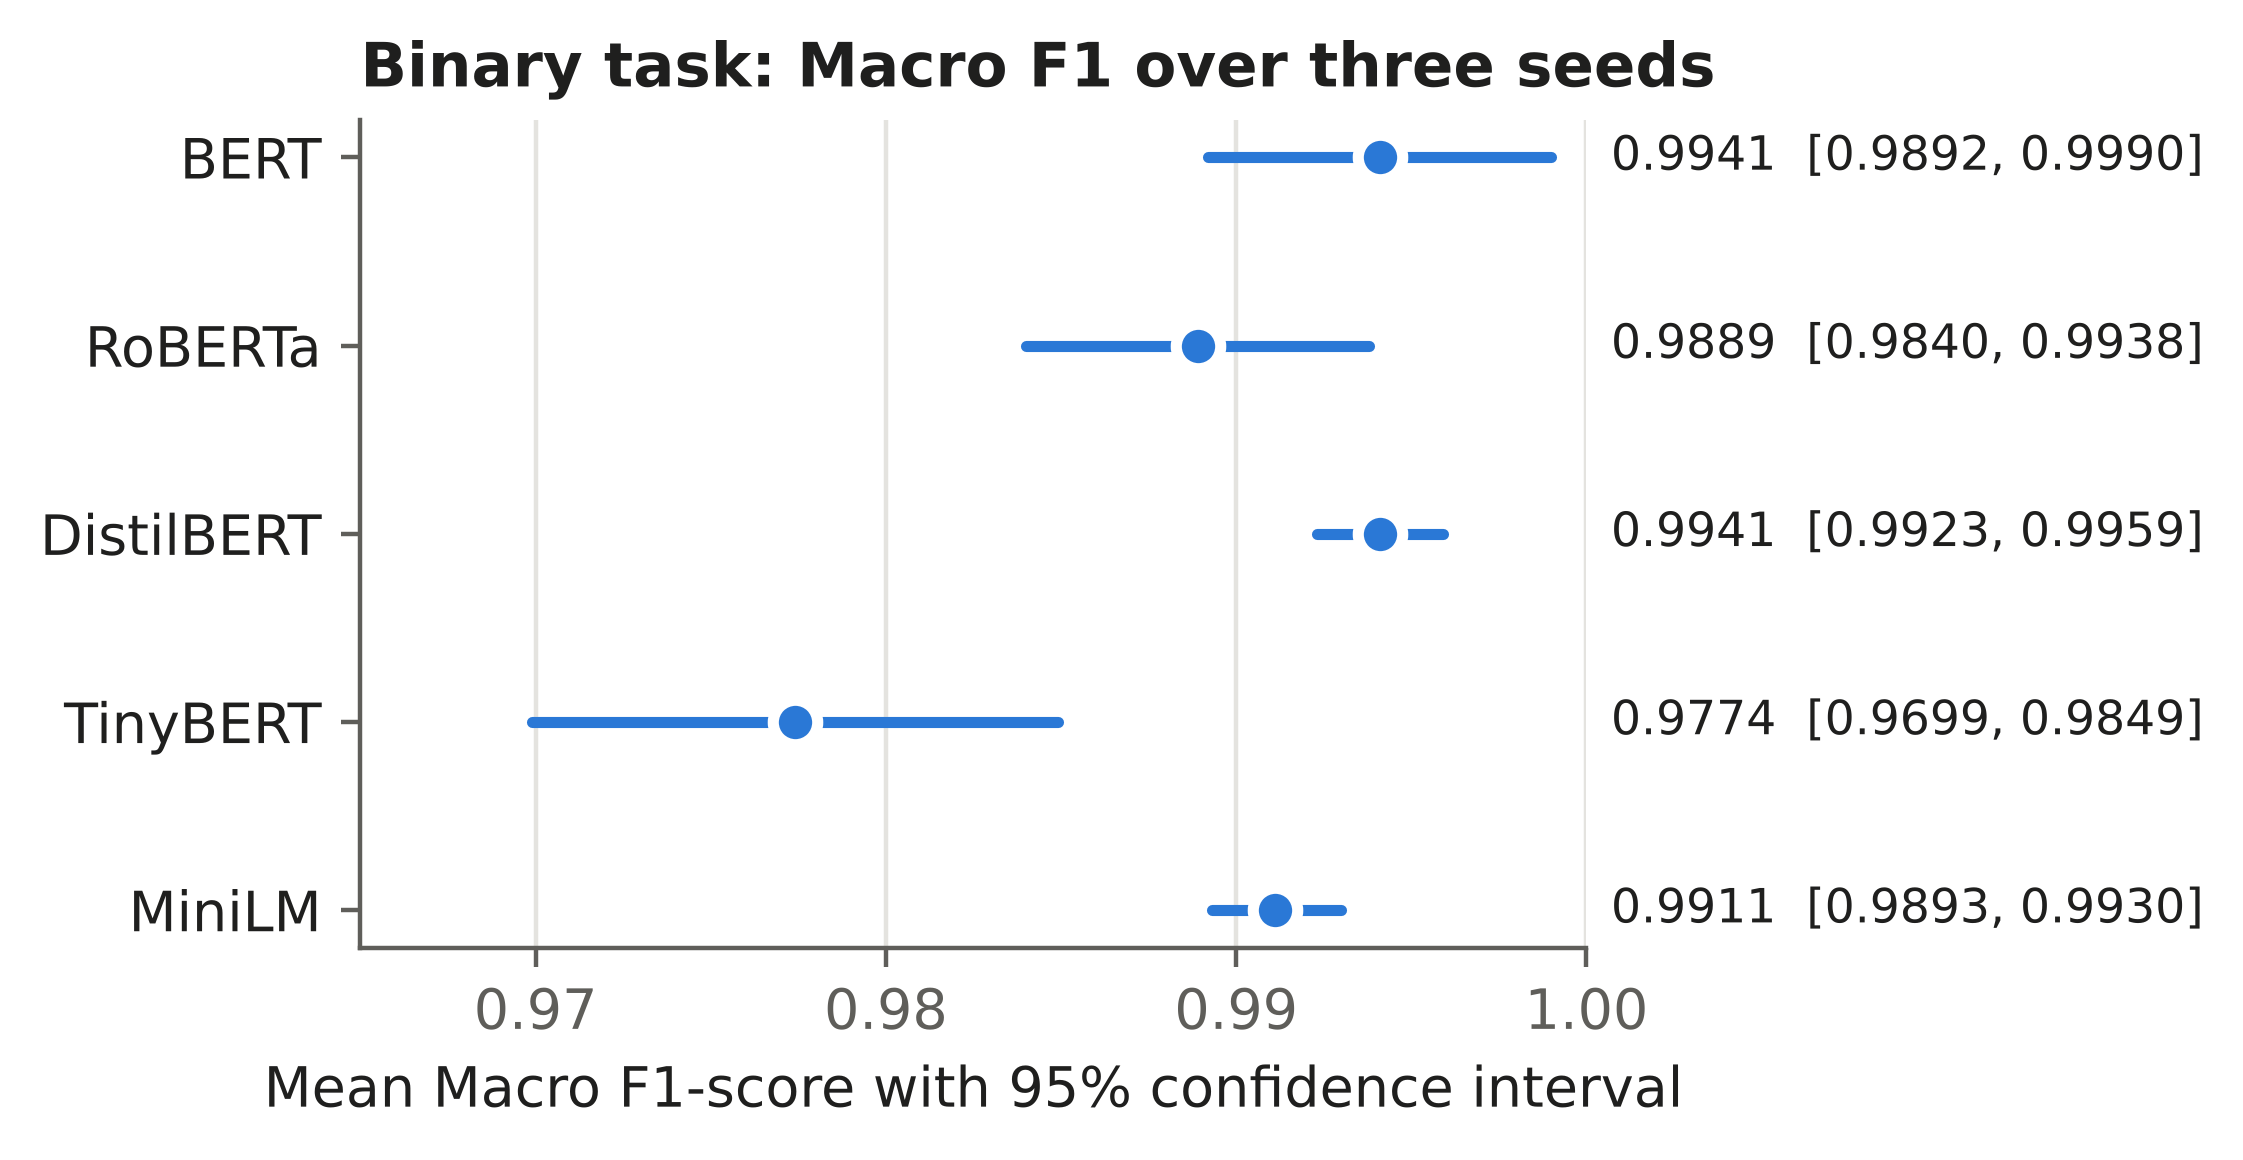
\includegraphics[width=\columnwidth]{fig2_binary_ci.png}
\caption{Macro F1-score for binary sarcasm detection\rcx{R5C9,R7C2}{ under Protocol A} across all Transformer Language Models. Error bars denote 95\% confidence intervals computed over three random seeds.\rcx{R7C7}{ The figure was regenerated so that its title is no longer cut off and its axis does not extend beyond 1.0.}}
\rcmark{R7C7}
\label{fig:bin-ci}
\end{figure}

\rcrep{R5C11}{Figure 2}{Figure~\ref{fig:bin-ci}} presents the Macro F1-scores with 95\% confidence intervals across all five architectures. The figure shows that the confidence intervals of BERT, RoBERTa, DistilBERT, and MiniLM overlap substantially, whereas the interval for TinyBERT is clearly separated from the others.

\begin{keyfinding}{Key Finding 1}\label{box:kf1}
All five Transformer architectures achieve high predictive performance in separating sarcastic from non-sarcastic app reviews\rcrep{R7C6}{, which indicates that pretrained contextual language models can capture the polarity shifts and implicit sentiment contradictions that characterize sarcastic expressions.}{.} BERT and DistilBERT obtain the highest mean Macro F1-score of 0.9941, followed by MiniLM at 0.9911 and RoBERTa at 0.9889. The confidence intervals of these four models overlap, and the statistical analysis reported in \rcrep{R5C11}{Section 6.1}{Section~\ref{sec:stats}} shows that \rcrep{R5C10}{the differences among them are not consistently distinguishable across seeds, although some pairs do reach significance at individual seeds}{no difference among them survives Holm correction for multiple comparisons, although some pairs reach nominal significance at individual seeds}. We therefore do not claim that any one of these four architectures outperforms the others on this task, and we note that a three-seed evaluation establishes the instability of the ordering rather than the equivalence of the models. TinyBERT reaches a mean Macro F1-score of 0.9774, which remains high in absolute terms but is \rcrep{R5C10}{consistently and significantly lower than that of the other four models}{significantly lower than that of BERT and DistilBERT at every seed after correction}. The practical implication is that the choice among BERT, RoBERTa, DistilBERT, and MiniLM for binary sarcasm detection can be governed primarily by computational cost rather than by predictive performance, because the predictive differences are not statistically supported. \rc{R7C6}{These scores should also be read alongside Section~\ref{sec:baselines}, which shows that a TF-IDF logistic regression baseline already reaches a Macro F1-score of 0.9673 on this task, so the near-perfect scores show that the binary class boundary of this benchmark is captured reliably rather than that the models resolve sarcasm in general.}
\end{keyfinding}

\rcrep{R5C11}{Figure 3}{Figure~\ref{fig:cm-roberta}} presents the confusion matrix of RoBERTa for seed 42, regenerated directly from the stored per-sample predictions of that run. The matrix is dominated by its diagonal, with 976 of 981 non-sarcastic reviews and 506 of 519 sarcastic reviews classified correctly. The residual errors \rcrep{R7C7}{are approximately balanced between false positives and false negatives}{consist of 5 false positives and 13 false negatives}, and manual inspection of the stored error cases indicates that they concentrate on reviews in which sentiment inversion is implicit and no lexical contrast signal is present.

\begin{figure}[]
\centering
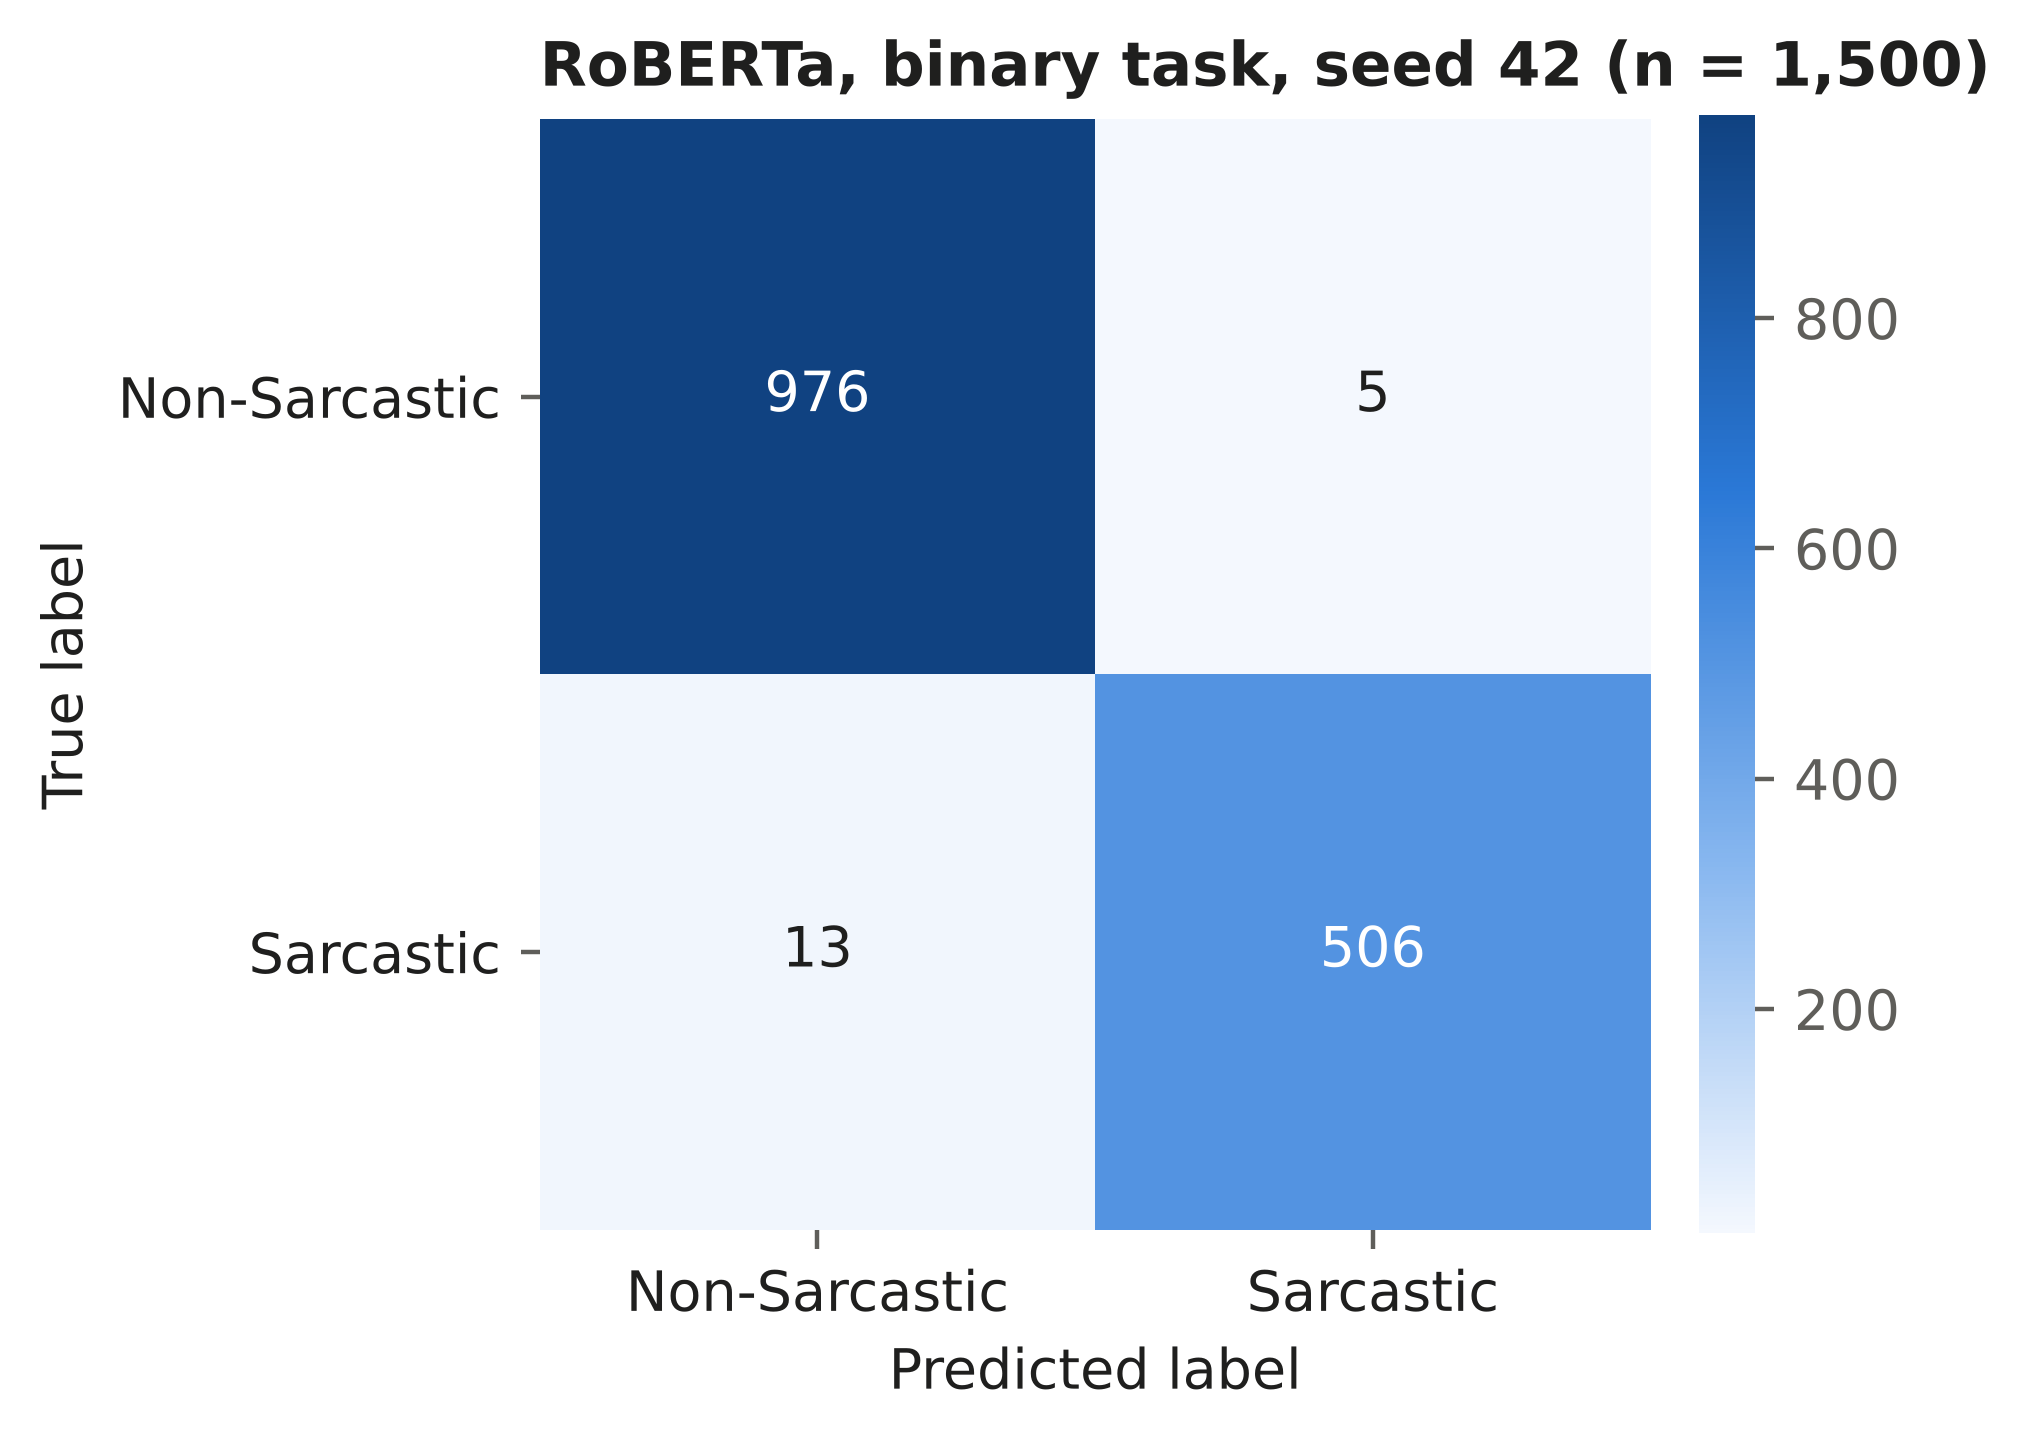
\includegraphics[width=0.75\columnwidth]{fig3_cm_roberta_binary.png}
\caption{Confusion matrix for RoBERTa on the binary task\rcx{R5C9,R7C2}{ under Protocol A}, seed 42, computed on the held-out test partition of 1,500 reviews.}
\label{fig:cm-roberta}
\end{figure}

\subsection{\texorpdfstring{\rcx{R5C11}{Sarcasm-Type Classification (RQ2)}}{Sarcasm-Type Classification (RQ2)}}
\label{sec:rq2}
\begin{rqbox}
\textbf{RQ2:} \textit{How well do transformer-based models capture and differentiate \rcrep{R5C11}{multiple types of sarcasm}{the five sarcasm types} in app reviews\rc{R5C11}{, and what effect does an optimized FlashAttention implementation have on their predictive performance and on their computational cost in this fine-grained setting}?}
\end{rqbox}

Fine-grained sarcasm-type classification is inherently more demanding than binary detection because it requires the model to separate categories that share lexical surface patterns and differ mainly in pragmatic intent. As described in \rcrep{R5C11}{Section 3.3}{Section~\ref{sec:dataset}}, this task is defined over the 3,460 reviews \rcrep{R5C9,R7C2}{that were annotated as sarcastic}{of the sarcasm-type file}, and the label space contains the five sarcasm types only. The held-out test partition contains 519 reviews. \rcrep{R5C11}{Table 7}{Table~\ref{tab:type-perclass}} reports the per-class results and \rcrep{R5C11}{Table 8}{Table~\ref{tab:type-agg}} the aggregated results. \rc{R5C11}{The effect of FlashAttention on this task is reported in Section~\ref{sec:efficiency-type}.}

\begin{table}[t]
\caption{Sarcasm-type classification\rcx{R5C9,R7C2}{ under Protocol A}: per-class results averaged over three random seeds (\rcx{R7C7}{eager} attention, NVIDIA T4). Support values are the \rcx{R7C7}{class counts of the held-out test partition, which are identical across seeds}.}
\label{tab:type-perclass}
\centering\small
\begin{tabular}{llccc}
\toprule
Model & Sarcasm type & Precision & Recall & F1-score \\
\midrule
\multirow{5}{*}{BERT} & Humor \rce{($n=257$)} & 0.949 & 0.895 & 0.921 \\
 & Irony \rce{($n=80$)} & 0.778 & 0.805 & 0.790 \\
 & Flattery \rce{($n=77$)} & 0.933 & 0.909 & 0.921 \\
 & Self-Deprecation \rce{($n=65$)} & 0.739 & 0.913 & 0.815 \\
 & Passive-Aggression \rce{($n=40$)} & 0.725 & 0.683 & 0.702 \\
\midrule
\multirow{5}{*}{RoBERTa} & Humor \rce{($n=257$)} & 0.958 & 0.886 & 0.920 \\
 & Irony \rce{($n=80$)} & 0.726 & 0.809 & 0.762 \\
 & Flattery \rce{($n=77$)} & 0.929 & 0.887 & 0.907 \\
 & Self-Deprecation \rce{($n=65$)} & 0.719 & 0.826 & 0.763 \\
 & Passive-Aggression \rce{($n=40$)} & 0.666 & 0.708 & 0.686 \\
\midrule
\multirow{5}{*}{DistilBERT} & Humor \rce{($n=257$)} & 0.949 & 0.900 & 0.924 \\
 & Irony \rce{($n=80$)} & 0.764 & 0.801 & 0.782 \\
 & Flattery \rce{($n=77$)} & 0.968 & 0.909 & 0.937 \\
 & Self-Deprecation \rce{($n=65$)} & 0.729 & 0.918 & 0.812 \\
 & Passive-Aggression \rce{($n=40$)} & 0.710 & 0.658 & 0.681 \\
\midrule
\multirow{5}{*}{TinyBERT} & Humor \rce{($n=257$)} & 0.943 & 0.799 & 0.864 \\
 & Irony \rce{($n=80$)} & 0.665 & 0.472 & 0.543 \\
 & Flattery \rce{($n=77$)} & 0.731 & 0.918 & 0.813 \\
 & Self-Deprecation \rce{($n=65$)} & 0.566 & 0.918 & 0.694 \\
 & Passive-Aggression \rce{($n=40$)} & 0.613 & 0.617 & 0.614 \\
\midrule
\multirow{5}{*}{MiniLM} & Humor \rce{($n=257$)} & 0.949 & 0.871 & 0.909 \\
 & Irony \rce{($n=80$)} & 0.738 & 0.772 & 0.754 \\
 & Flattery \rce{($n=77$)} & 0.945 & 0.905 & 0.924 \\
 & Self-Deprecation \rce{($n=65$)} & 0.708 & 0.892 & 0.789 \\
 & Passive-Aggression \rce{($n=40$)} & 0.641 & 0.700 & 0.669 \\
\bottomrule
\end{tabular}
\end{table}

\begin{table}[t]
\caption{Sarcasm-type classification\rcx{R5C9,R7C2}{ under Protocol A}: aggregated results over three random seeds, reported as mean and standard deviation with the 95\% confidence interval of the Macro F1-score. Best value in each column is shown in bold.}
\label{tab:type-agg}
\centering\small
\begin{adjustbox}{max width=\textwidth}
\begin{tabular}{lcccc}
\toprule
Model & Accuracy & Macro F1 & Weighted F1 & Macro F1 95\% CI \\
\midrule
BERT & 0.8690 $\pm$ 0.0051 & \textbf{0.8301} $\pm$ 0.0072 & 0.8708 $\pm$ 0.0056 & [0.8122, 0.8480] \\
RoBERTa & 0.8529 $\pm$ 0.0059 & 0.8078 $\pm$ 0.0091 & 0.8562 $\pm$ 0.0061 & [0.7852, 0.8304] \\
DistilBERT & \textbf{0.8696} $\pm$ 0.0080 & 0.8273 $\pm$ 0.0194 & \textbf{0.8712} $\pm$ 0.0088 & [0.7790, 0.8755] \\
TinyBERT & 0.7669 $\pm$ 0.0495 & 0.7058 $\pm$ 0.0616 & 0.7665 $\pm$ 0.0528 & [0.5528, 0.8588] \\
MiniLM & 0.8504 $\pm$ 0.0128 & 0.8092 $\pm$ 0.0223 & 0.8537 $\pm$ 0.0130 & [0.7540, 0.8645] \\
\bottomrule
\end{tabular}
\end{adjustbox}
\end{table}

\begin{figure}[]
\centering
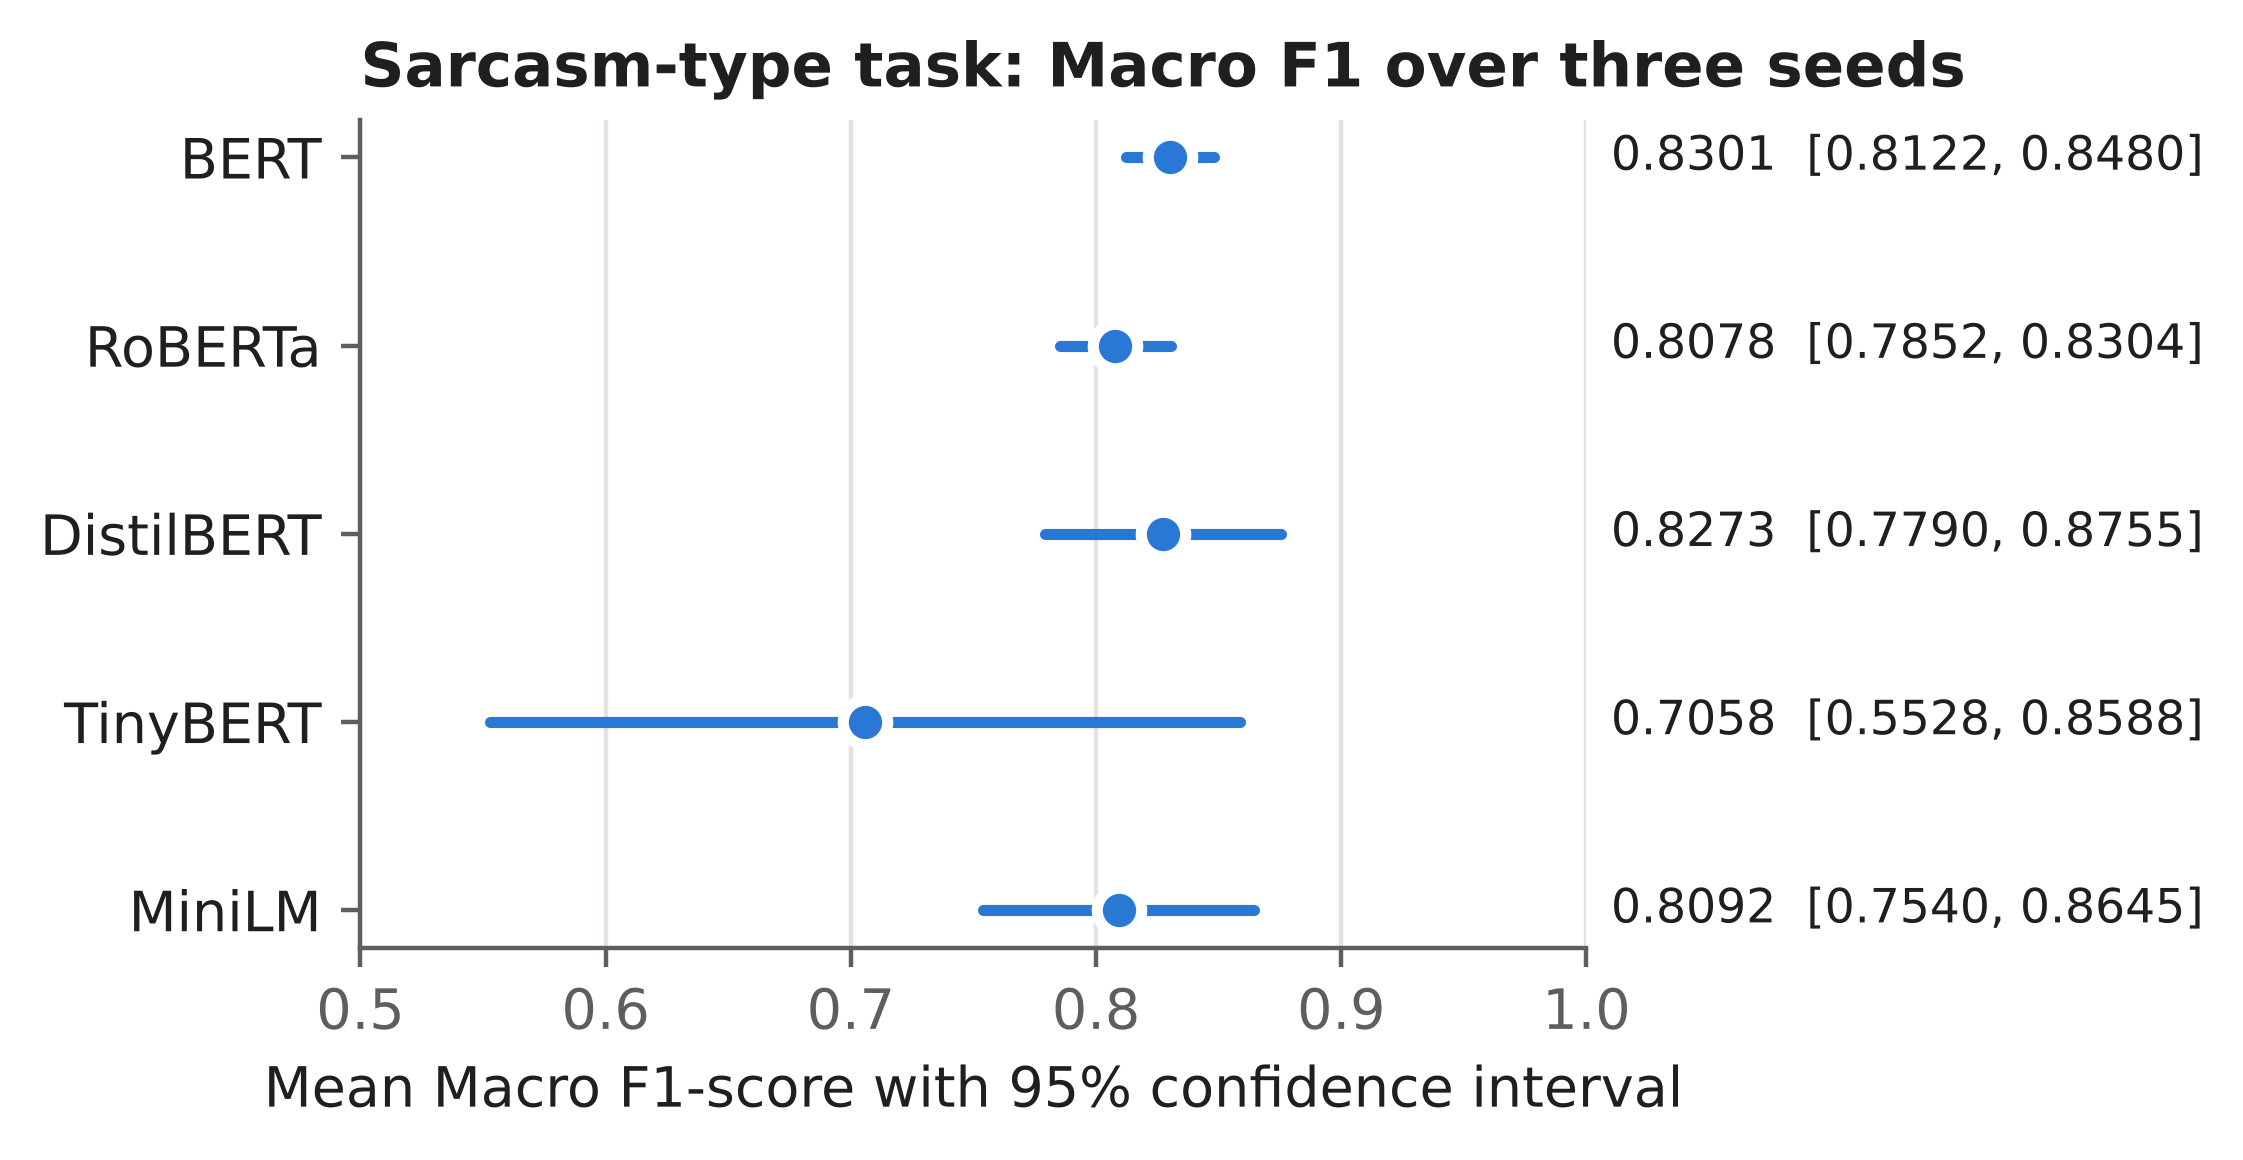
\includegraphics[width=\columnwidth]{fig4_type_ci.png}
\caption{Macro F1-score for sarcasm-type classification\rcx{R5C9,R7C2}{ under Protocol A} across all Transformer Language Models. Error bars denote 95\% confidence intervals computed over three random seeds.}
\label{fig:type-ci}
\end{figure}

\begin{figure}[]
\centering
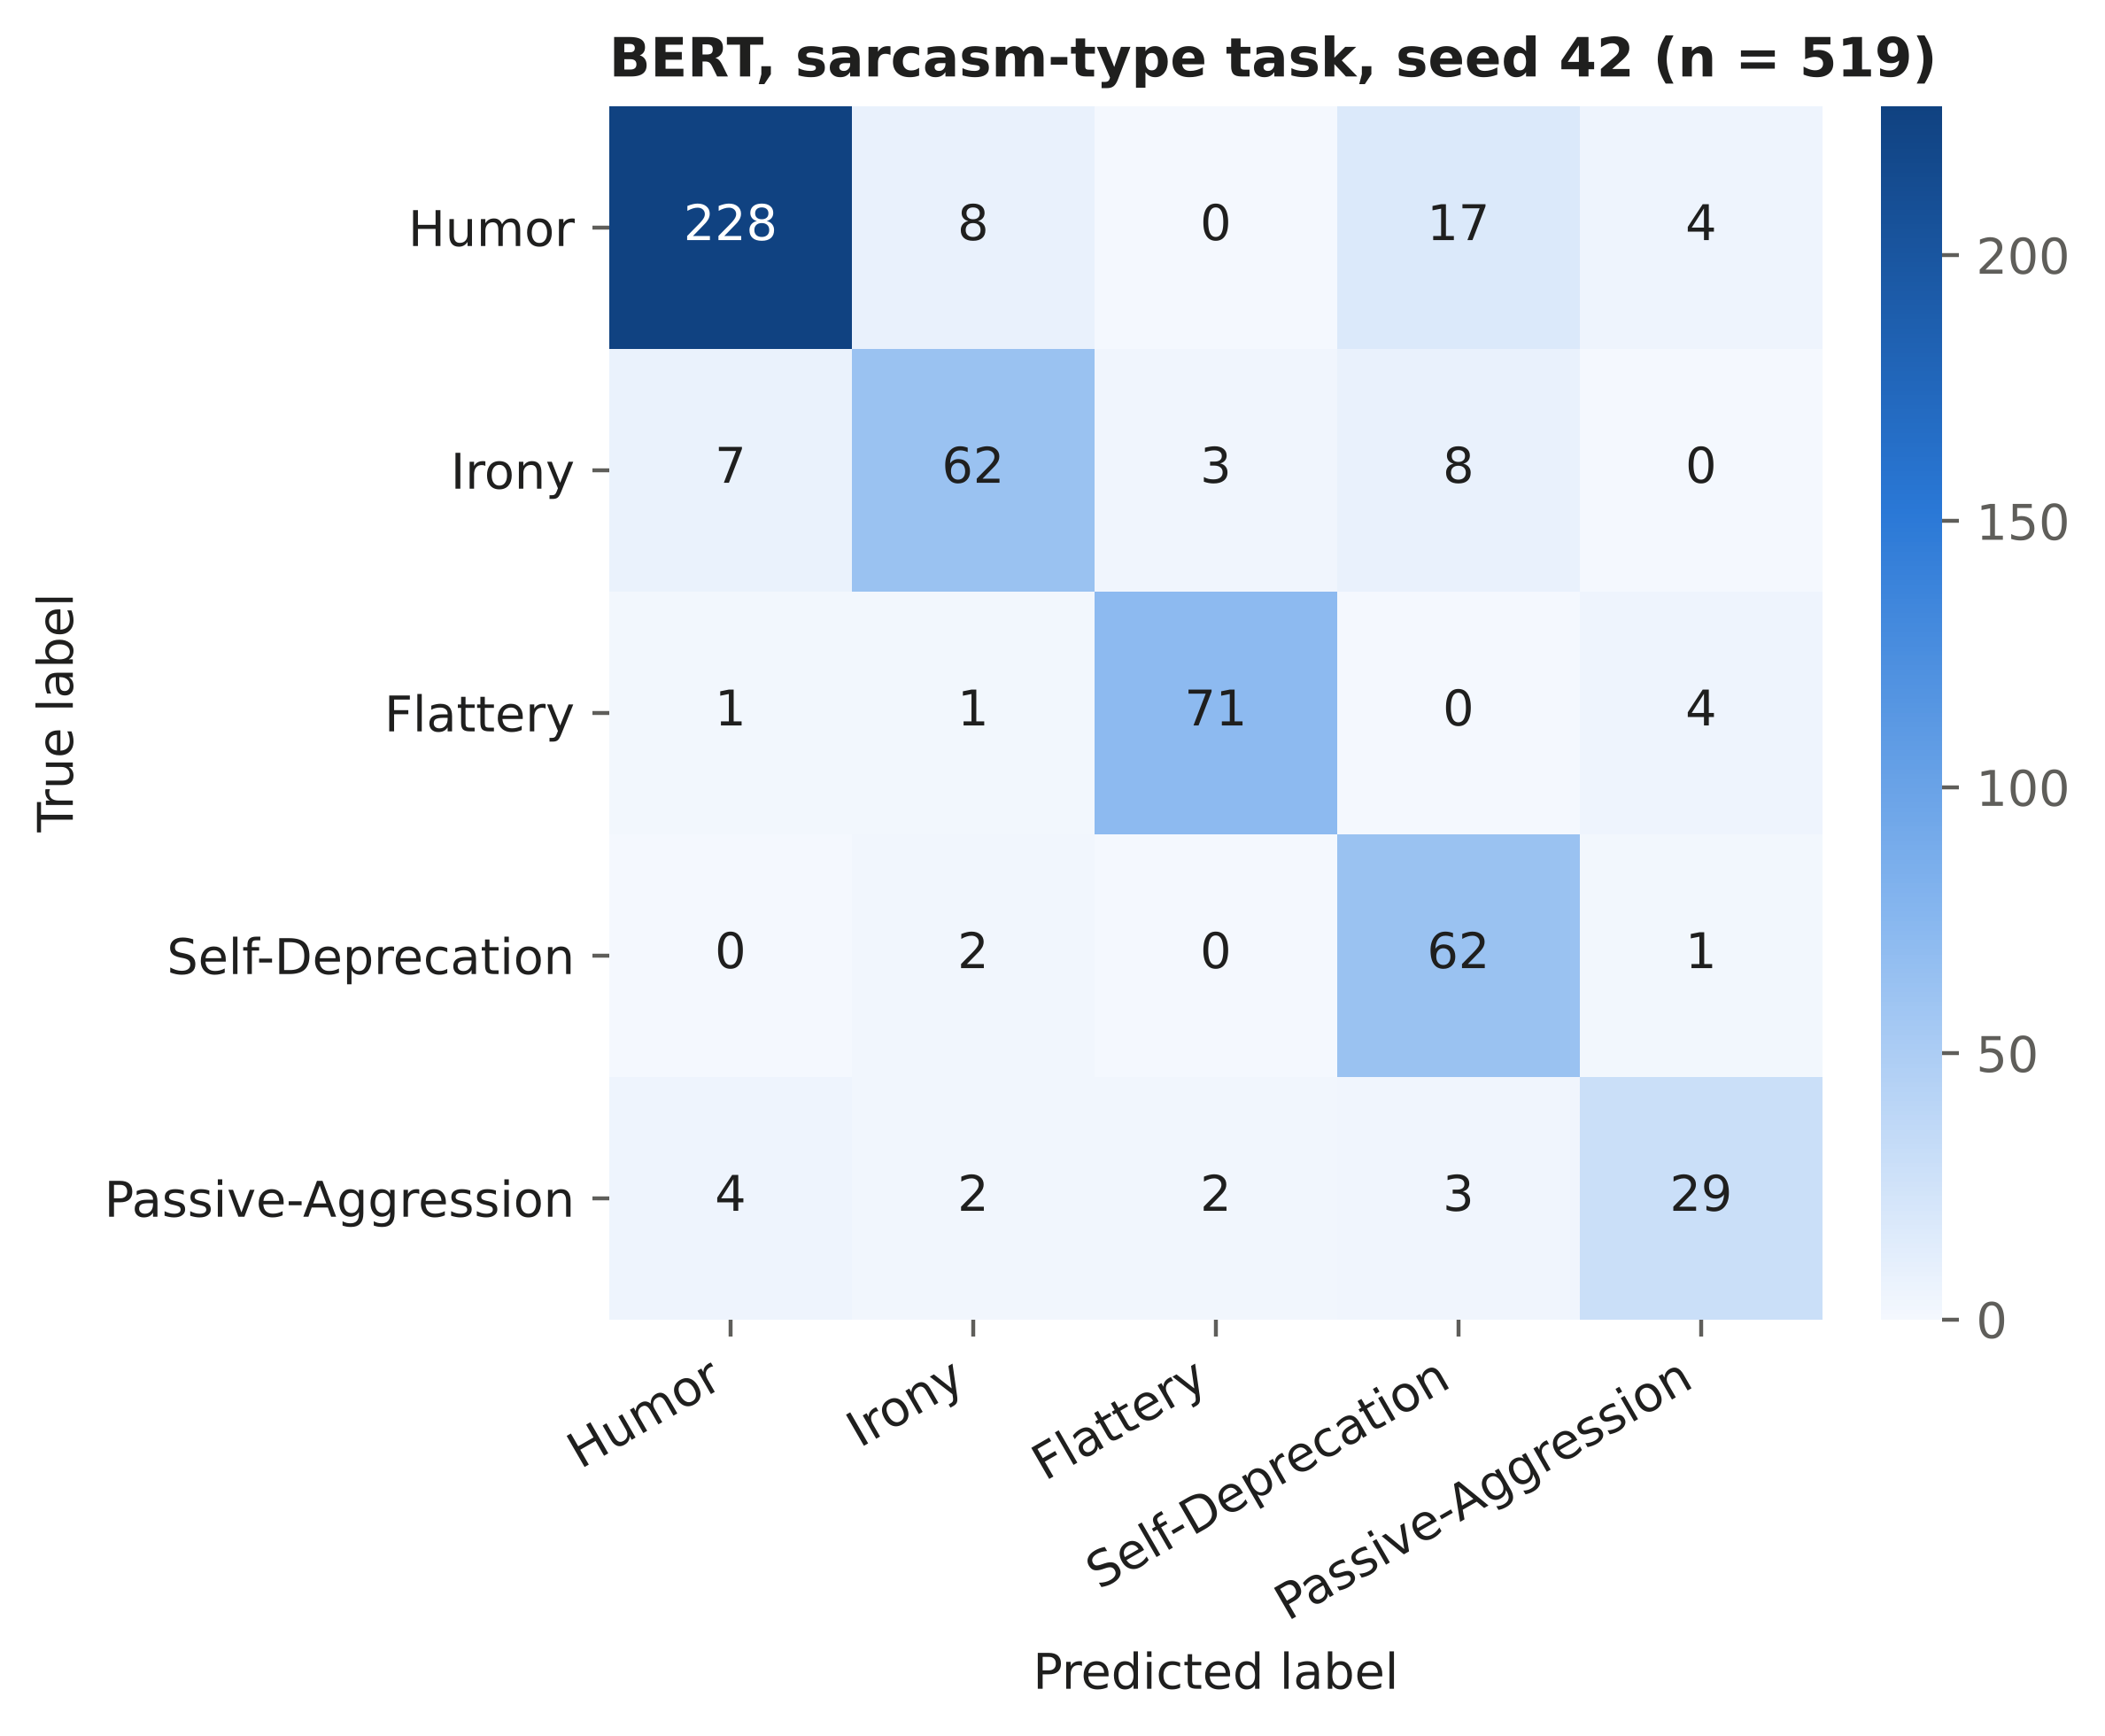
\includegraphics[width=0.85\columnwidth]{fig5_cm_bert_type.png}
\caption{Confusion matrix for BERT on the sarcasm-type task\rcx{R5C9,R7C2}{ under Protocol A}, seed 42, computed on the held-out test partition of 519 reviews.}
\label{fig:cm-bert}
\end{figure}

\begin{keyfinding}{Key Finding 2}\label{box:kf2}
Sarcasm-type classification is markedly harder than binary detection. BERT obtains the highest mean Macro F1-score of 0.8301, followed closely by DistilBERT at 0.8273, MiniLM at 0.8092, and RoBERTa at 0.8078, while TinyBERT reaches 0.7058 with a considerably larger standard deviation of 0.0616. The gap of approximately sixteen Macro F1 points between the two tasks quantifies the additional difficulty of separating sarcasm types once the sarcastic and non-sarcastic decision has already been made.

The per-class results in \rcrep{R5C11}{Table 7}{Table~\ref{tab:type-perclass}} explain where the difficulty lies. Humor and Flattery are recognized reliably by every model except TinyBERT, with F1-scores between 0.907 and 0.937, because these categories carry comparatively distinctive lexical and stylistic markers. \rcrep{R7C7}{Passive-Aggression is the weakest category for every architecture, with F1-scores between 0.614 and 0.702, and Irony is the second weakest. Both categories are characterized by low precision relative to recall for the minority classes, which indicates that the models overassign these labels to reviews whose pragmatic intent is ambiguous.}{Passive-Aggression is the weakest category for four of the five architectures, with F1-scores between 0.669 and 0.702, and for TinyBERT it is surpassed in difficulty only by Irony (0.543 against 0.614). The pattern of low precision relative to recall appears consistently for Self-Deprecation, whose precision lies between 0.566 and 0.739 while its recall lies between 0.826 and 0.918 for every architecture, so the models assign this label to many reviews that the annotators placed elsewhere.} The confusion matrix in \rcrep{R5C11}{Figure 5}{Figure~\ref{fig:cm-bert}} shows that the residual errors occur predominantly between semantically adjacent categories rather than between conceptually distinct ones\rc{R7C7}{, its largest off-diagonal cell being the 17 Humor reviews predicted as Self-Deprecation}. \rc{R5C9,R7C2}{This pattern is consistent with the annotation audit of Section~\ref{sec:duplicates}, in which Self-Deprecation is involved in the two most frequent pairs of conflicting labels.} This analysis is derived from the stored per-class metrics and confusion matrices. We did not conduct feature-attribution analysis, adversarial perturbation testing or a systematic manual study of shortcut lexical cues, and we therefore make no claim about which surface features the models rely upon; these analyses are identified as future work in \rcrep{R5C11}{Section 8}{Section~\ref{sec:threats}}\rc{R7C6}{, while Section~\ref{sec:baselines} reports what a purely lexical model achieves on the same partitions}.

The variance across seeds is also informative. TinyBERT shows a Macro F1 standard deviation of 0.0616 and a 95\% confidence interval spanning [0.5528, 0.8588], which indicates that the smallest architecture is not merely weaker on this task but also unstable when the minority classes contain only a few dozen training instances. This instability is a deployment-relevant property that a single-run evaluation would not have exposed.
\end{keyfinding}

\subsection{Statistical Validation of Model Differences}
\label{sec:stats}
Reviewers of the previous version observed that averaged results alone cannot establish whether the differences between architectures are meaningful. To address this concern, we conducted paired statistical testing on the stored per-sample predictions\rc{R5C9,R7C2}{ of Protocol A}. For every pair of models and every seed, we computed a paired bootstrap test on the Macro F1 difference using 2,500 resamples of the test set, together with an exact McNemar test on the matched correct and incorrect decision counts. This produced sixty paired comparisons in total, comprising ten model pairs, three seeds, and two tasks. The null hypothesis in each case is that the two models have equal performance on the evaluated population\rcrep{R5C10}{, and no correction for multiple comparisons was applied because the tests are reported as a descriptive stability analysis rather than as a family-wise confirmatory procedure.}{. To control the family-wise error rate across the sixty comparisons, we applied the Holm correction \citep{holm1979simple} to the McNemar $p$-values and treated all sixty tests as one family.} \rcrep{R5C11}{Table 9}{Table~\ref{tab:paired}} summarizes the outcome\rc{R5C10}{ before and after correction}, and the complete per-seed output\rc{R5C10}{, including every adjusted $p$-value,} is provided as supplementary material.

The statistical evidence supports a single consistent conclusion. Every comparison involving TinyBERT is significant at $\alpha = 0.05$ for all three seeds on both tasks\rc{R5C10}{ before correction}, and in each of these cases the bootstrap confidence interval excludes zero. \rc{R5C10}{After Holm correction, 18 of these 24 comparisons remain significant, including all twelve comparisons of TinyBERT with BERT and with DistilBERT on both tasks, while the comparisons of TinyBERT with RoBERTa and with MiniLM remain significant at one or two seeds per task.} For example, the difference between DistilBERT and TinyBERT on the binary task has McNemar $p$-values of $2.4\times10^{-7}$, $2.1\times10^{-5}$, and $2.2\times10^{-7}$ across the three seeds\rc{R5C10}{, and Holm-adjusted values of $1.3\times10^{-5}$, $1.0\times10^{-3}$, and $1.2\times10^{-5}$}. By contrast, the comparisons among BERT, RoBERTa, DistilBERT and MiniLM are not stable across seeds. BERT and DistilBERT are never distinguishable on either task. BERT and RoBERTa are distinguishable on the binary task at two of the three seeds, with McNemar $p$-values of 0.039, 0.42 and 0.022, and at none of the seeds on the sarcasm-type task. \rcrep{R5C10}{BERT and MiniLM, and DistilBERT and MiniLM, each reach significance at one seed of three on the binary task.}{RoBERTa and DistilBERT, and BERT and MiniLM, each reach significance at one seed on each task, and DistilBERT and MiniLM at one seed on the sarcasm-type task only, so that 7 of the 36 comparisons among these four architectures are significant before correction. After Holm correction none of these 36 comparisons remains significant, the smallest adjusted $p$-value being 0.17.} These comparisons therefore yield different conclusions depending on the random initialization, which is the pattern that a single-run evaluation would have concealed.

We therefore summarize the statistical evidence as follows. TinyBERT performs significantly worse than \rcrep{R5C10}{each of the four stronger architectures, and this holds at every seed on both tasks}{BERT and DistilBERT at every seed on both tasks, and worse than RoBERTa and MiniLM at most seeds, after correction for multiple comparisons}. The differences among BERT, RoBERTa, DistilBERT and MiniLM are considerably smaller\rce{,} \rcrep{R5C10}{and are not stable across seeds. Some of these comparisons do reach significance at individual seeds, and we}{are not stable across seeds and do not survive the correction. We} do not claim that these four models are statistically indistinguishable in an absolute sense, since a three-seed evaluation cannot establish equivalence. The appropriate reading is that the observed ordering among the four stronger models is not reproducible across random initializations and should not be relied upon, whereas the deficit of TinyBERT is reproducible. Practically, this means that a selection made among the four stronger architectures on the basis of a single run would not be well founded, and that computational cost is a more defensible selection criterion for them, which is the question addressed by RQ3. \rc{R5C9,R7C2}{Section~\ref{sec:robust-dedup} repeats this analysis on the deduplicated partitions.}

\begin{table*}[t]
\caption{Paired statistical comparison of model pairs\rcx{R5C9,R7C2}{ under Protocol A}. \rcrep{R5C10}{The mean absolute Macro F1 difference is averaged over three seeds.}{The third column is the absolute value of the seed-averaged signed Macro F1 difference.} The final \rcrep{R5C10}{two}{three} columns report the number of seeds out of three for which the McNemar test rejected the null hypothesis at the 0.05 level\rcx{R5C10}{ before correction and after Holm correction over all sixty comparisons}, and the number of seeds for which the bootstrap 95\% confidence interval of the difference contained zero.}
\rcmark{R5C10}
\label{tab:paired}
\centering\small
\begin{adjustbox}{max width=\textwidth}
\begin{tabular}{llcccc}
\toprule
Task & Model pair & $|$Mean Macro F1 diff.$|$ & McNemar $p<0.05$ & \rc{R5C10}{Holm-adjusted $p<0.05$} & CI contains 0 \\
\midrule
Binary & BERT vs.\ DistilBERT & 0.0000 & 0/3 & \rcm{R5C10}{0/3} & 3/3 \\
Binary & RoBERTa vs.\ MiniLM & 0.0022 & 0/3 & \rcm{R5C10}{0/3} & 3/3 \\
Binary & BERT vs.\ MiniLM & 0.0030 & 1/3 & \rcm{R5C10}{0/3} & 2/3 \\
Binary & DistilBERT vs.\ MiniLM & 0.0030 & 0/3 & \rcm{R5C10}{0/3} & 2/3 \\
Binary & BERT vs.\ RoBERTa & 0.0052 & 2/3 & \rcm{R5C10}{0/3} & 1/3 \\
Binary & RoBERTa vs.\ DistilBERT & 0.0052 & 1/3 & \rcm{R5C10}{0/3} & 2/3 \\
Binary & RoBERTa vs.\ TinyBERT & 0.0115 & 3/3 & \rcm{R5C10}{1/3} & 0/3 \\
Binary & TinyBERT vs.\ MiniLM & 0.0137 & 3/3 & \rcm{R5C10}{2/3} & 0/3 \\
Binary & BERT vs.\ TinyBERT & 0.0167 & 3/3 & \rcm{R5C10}{3/3} & 0/3 \\
Binary & DistilBERT vs.\ TinyBERT & 0.0167 & 3/3 & \rcm{R5C10}{3/3} & 0/3 \\
\midrule
Sarcasm type & RoBERTa vs.\ MiniLM & 0.0015 & 0/3 & \rcm{R5C10}{0/3} & 3/3 \\
Sarcasm type & BERT vs.\ DistilBERT & 0.0028 & 0/3 & \rcm{R5C10}{0/3} & 3/3 \\
Sarcasm type & DistilBERT vs.\ MiniLM & 0.0180 & 1/3 & \rcm{R5C10}{0/3} & 3/3 \\
Sarcasm type & RoBERTa vs.\ DistilBERT & 0.0195 & 1/3 & \rcm{R5C10}{0/3} & 2/3 \\
Sarcasm type & BERT vs.\ MiniLM & 0.0208 & 1/3 & \rcm{R5C10}{0/3} & 2/3 \\
Sarcasm type & BERT vs.\ RoBERTa & 0.0223 & 0/3 & \rcm{R5C10}{0/3} & 3/3 \\
Sarcasm type & RoBERTa vs.\ TinyBERT & 0.1020 & 3/3 & \rcm{R5C10}{2/3} & 0/3 \\
Sarcasm type & TinyBERT vs.\ MiniLM & 0.1035 & 3/3 & \rcm{R5C10}{1/3} & 0/3 \\
Sarcasm type & DistilBERT vs.\ TinyBERT & 0.1215 & 3/3 & \rcm{R5C10}{3/3} & 0/3 \\
Sarcasm type & BERT vs.\ TinyBERT & 0.1243 & 3/3 & \rcm{R5C10}{3/3} & 0/3 \\
\bottomrule
\end{tabular}
\end{adjustbox}
\end{table*}

\subsection{\texorpdfstring{\rcx{R5C11}{Computational Efficiency and FlashAttention (RQ3)}}{Computational Efficiency and FlashAttention (RQ3)}}
\label{sec:efficiency}
\begin{rqbox}
\textbf{RQ3:} \textit{\rcrep{R5C11}{How do different Transformer Language Models compare in terms of computational efficiency, including training time, inference latency, and memory usage, and to what extent does FlashAttention assess their suitability for deployment-oriented software analytics?}{How do the evaluated Transformer Language Models compare in terms of computational efficiency, measured as training time, inference latency and peak GPU memory consumption, and to what extent does an optimized FlashAttention implementation reduce these costs?}}
\end{rqbox}

While RQ1 and RQ2 evaluate predictive effectiveness, RQ3 examines deployment-oriented computational efficiency\rcdel{R7C7}{.}. In \rcrep{R5C1,R7C5}{continuous software analytics environments}{software analytics environments that process reviews repeatedly}, training cost, inference latency, and memory footprint influence operational usability as strongly as accuracy. FlashAttention is incorporated in this study as an existing optimization mechanism rather than as a modification of the transformer architecture, and the objective of RQ3 is therefore to quantify its practical effect on sarcasm detection rather than to propose a new attention mechanism.

The FlashAttention evaluation was conducted as a dedicated controlled experiment that is separate from the main model grid reported in \rcrep{R5C11}{Sections 6 and 6}{Sections~\ref{sec:rq1} and~\ref{sec:rq2}}. In each run the attention backend was verified programmatically before training, and only runs in which a forward pass completed under a FlashAttention-only backend were retained as FlashAttention runs. The comparison condition uses the eager attention implementation. \rcdel{R7C7}{Because the two tasks were executed on different available hardware, the binary and sarcasm-type efficiency results are reported separately and are not pooled.} The binary comparison was executed on an NVIDIA A100-SXM4-40GB device using the PyTorch scaled dot-product attention FlashAttention backend, and the sarcasm-type comparison was executed on an NVIDIA GeForce RTX 3060 Ti device using the FlashAttention-2 library, version 2.8.3.post1. Because the two experiments use different FlashAttention implementations as well as different hardware, their results are reported separately and their magnitudes are not comparable to one another. Latency values were measured over thirty timing runs following ten warm-up batches.

\subsubsection{Efficiency on the sarcasm-type task}
\label{sec:efficiency-type}
\rcrep{R5C11}{Table 10}{Table~\ref{tab:fa-type}} reports the sarcasm-type comparison, which is the more complete of the two because it includes memory profiling\rcdel{R7C4}{for both training and inference}\rc{R7C4}{ of training}\rc{R5C11}{, and Figures~\ref{fig:fa-time} to~\ref{fig:fa-latency} show training time, peak training memory and inference latency}.

\begin{table*}[t]
\caption{Verified FlashAttention-2 comparison on the sarcasm-type task. \rce{The} optimized condition uses the FlashAttention-2 library version 2.8.3.post1; \rce{the} baseline condition uses eager attention. NVIDIA RTX 3060 Ti, three seeds, mean values. Negative percentages denote reductions relative to the eager baseline.}
\label{tab:fa-type}
\centering\small
\begin{adjustbox}{max width=\textwidth}
\begin{tabular}{lcccccccc}
\toprule
 & \multicolumn{2}{c}{Macro F1} & \multicolumn{2}{c}{Training time (s)} & \multicolumn{2}{c}{Latency (ms)} & \multicolumn{2}{c}{Peak training memory (MB)} \\
\cmidrule(lr){2-3}\cmidrule(lr){4-5}\cmidrule(lr){6-7}\cmidrule(lr){8-9}
Model & Eager & Flash & Eager & Flash & Eager & Flash & Eager & Flash \\
\midrule
BERT & 0.8288 & 0.8271 & 122.14 & 105.24 ($-$13.8\%) & 25.98 & 21.26 ($-$18.2\%) & 2567.2 & 2257.3 ($-$12.1\%) \\
RoBERTa & 0.8306 & 0.8189 & 193.45 & 151.12 ($-$21.9\%) & 17.21 & 12.53 ($-$27.2\%) & 2436.2 & 2185.0 ($-$10.3\%) \\
DistilBERT & 0.8371 & 0.8457 & 66.06 & 58.61 ($-$11.3\%) & 15.45 & 13.19 ($-$14.6\%) & 1439.0 & 1292.6 ($-$10.2\%) \\
TinyBERT & 0.7473 & 0.7388 & 16.62 & 14.09 ($-$15.2\%) & 7.18 & 5.80 ($-$19.3\%) & 624.7 & 511.8 ($-$18.1\%) \\
MiniLM & 0.8180 & 0.8161 & 70.99 & 61.67 ($-$13.1\%) & 16.64 & 13.76 ($-$17.3\%) & 1123.0 & 954.9 ($-$15.0\%) \\
\bottomrule
\end{tabular}
\end{adjustbox}
\end{table*}

\begin{figure}[]
\centering
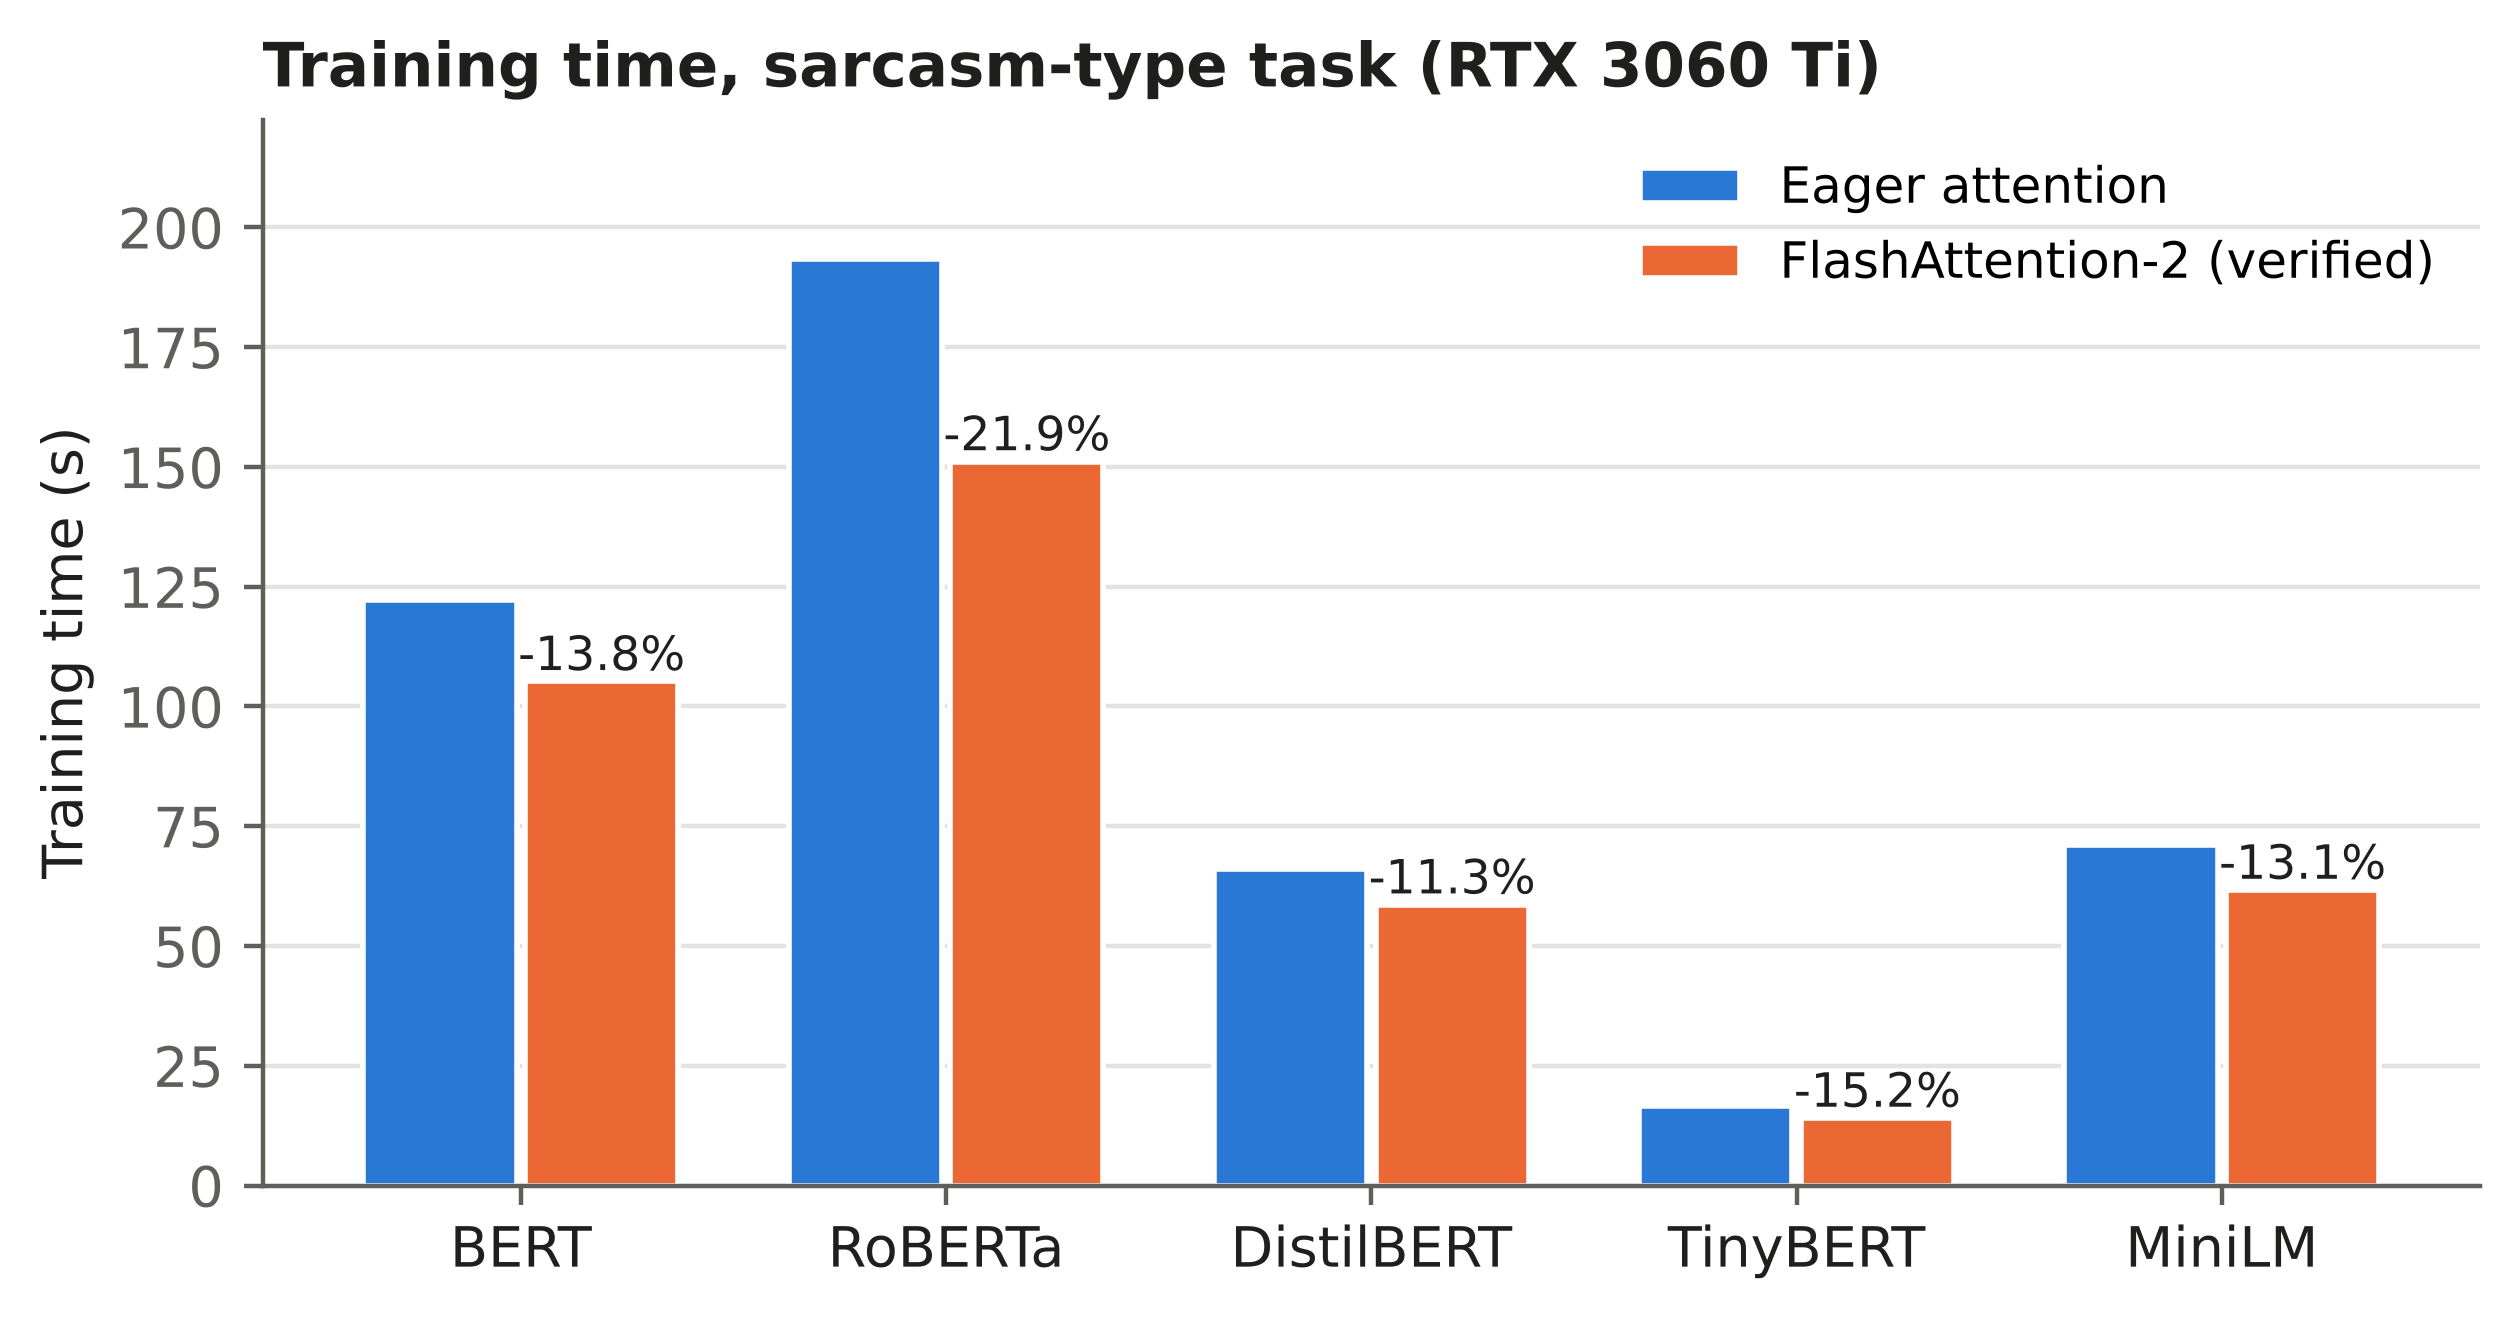
\includegraphics[width=\columnwidth]{fig6_fa_training_time.png}
\caption{Training time under eager attention and verified FlashAttention-2 on the sarcasm-type task.\rcx{R7C7}{ Labels give the change relative to eager attention.}}
\label{fig:fa-time}
\end{figure}

\begin{figure}[]
\centering
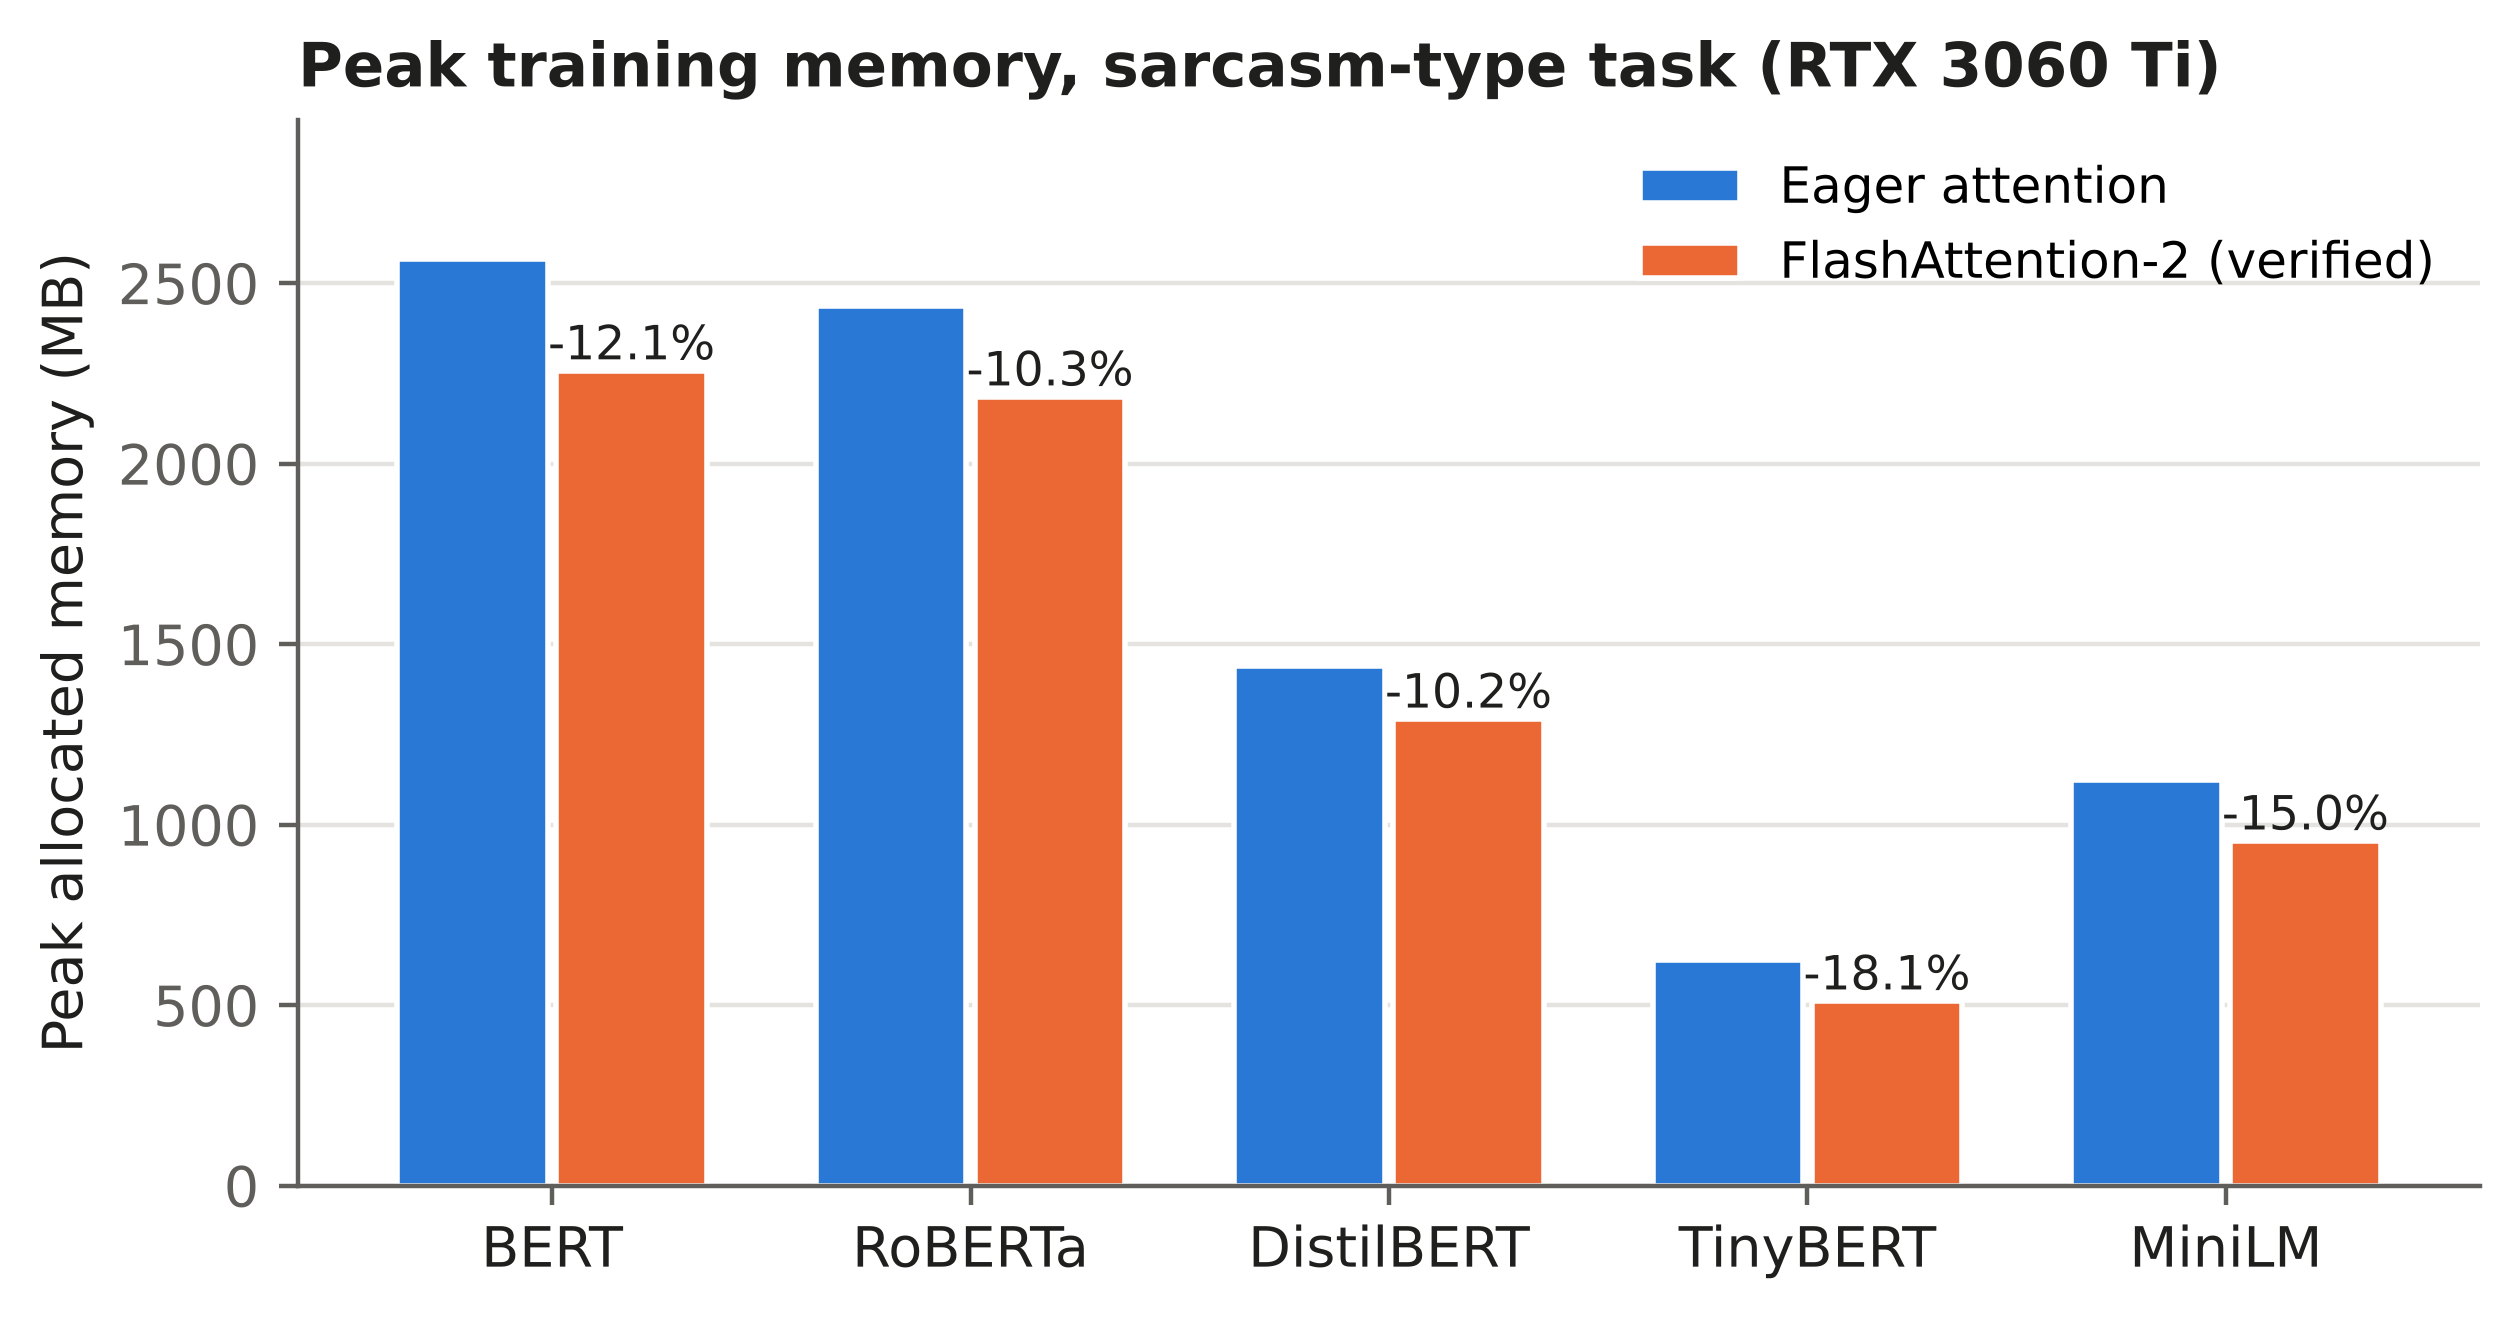
\includegraphics[width=\columnwidth]{fig7_fa_training_memory.png}
\caption{Peak allocated GPU training memory under eager attention and verified FlashAttention-2 on the sarcasm-type task.\rcx{R7C7}{ Labels give the change relative to eager attention.}}
\label{fig:fa-memory}
\end{figure}

\begin{figure}[]
\centering
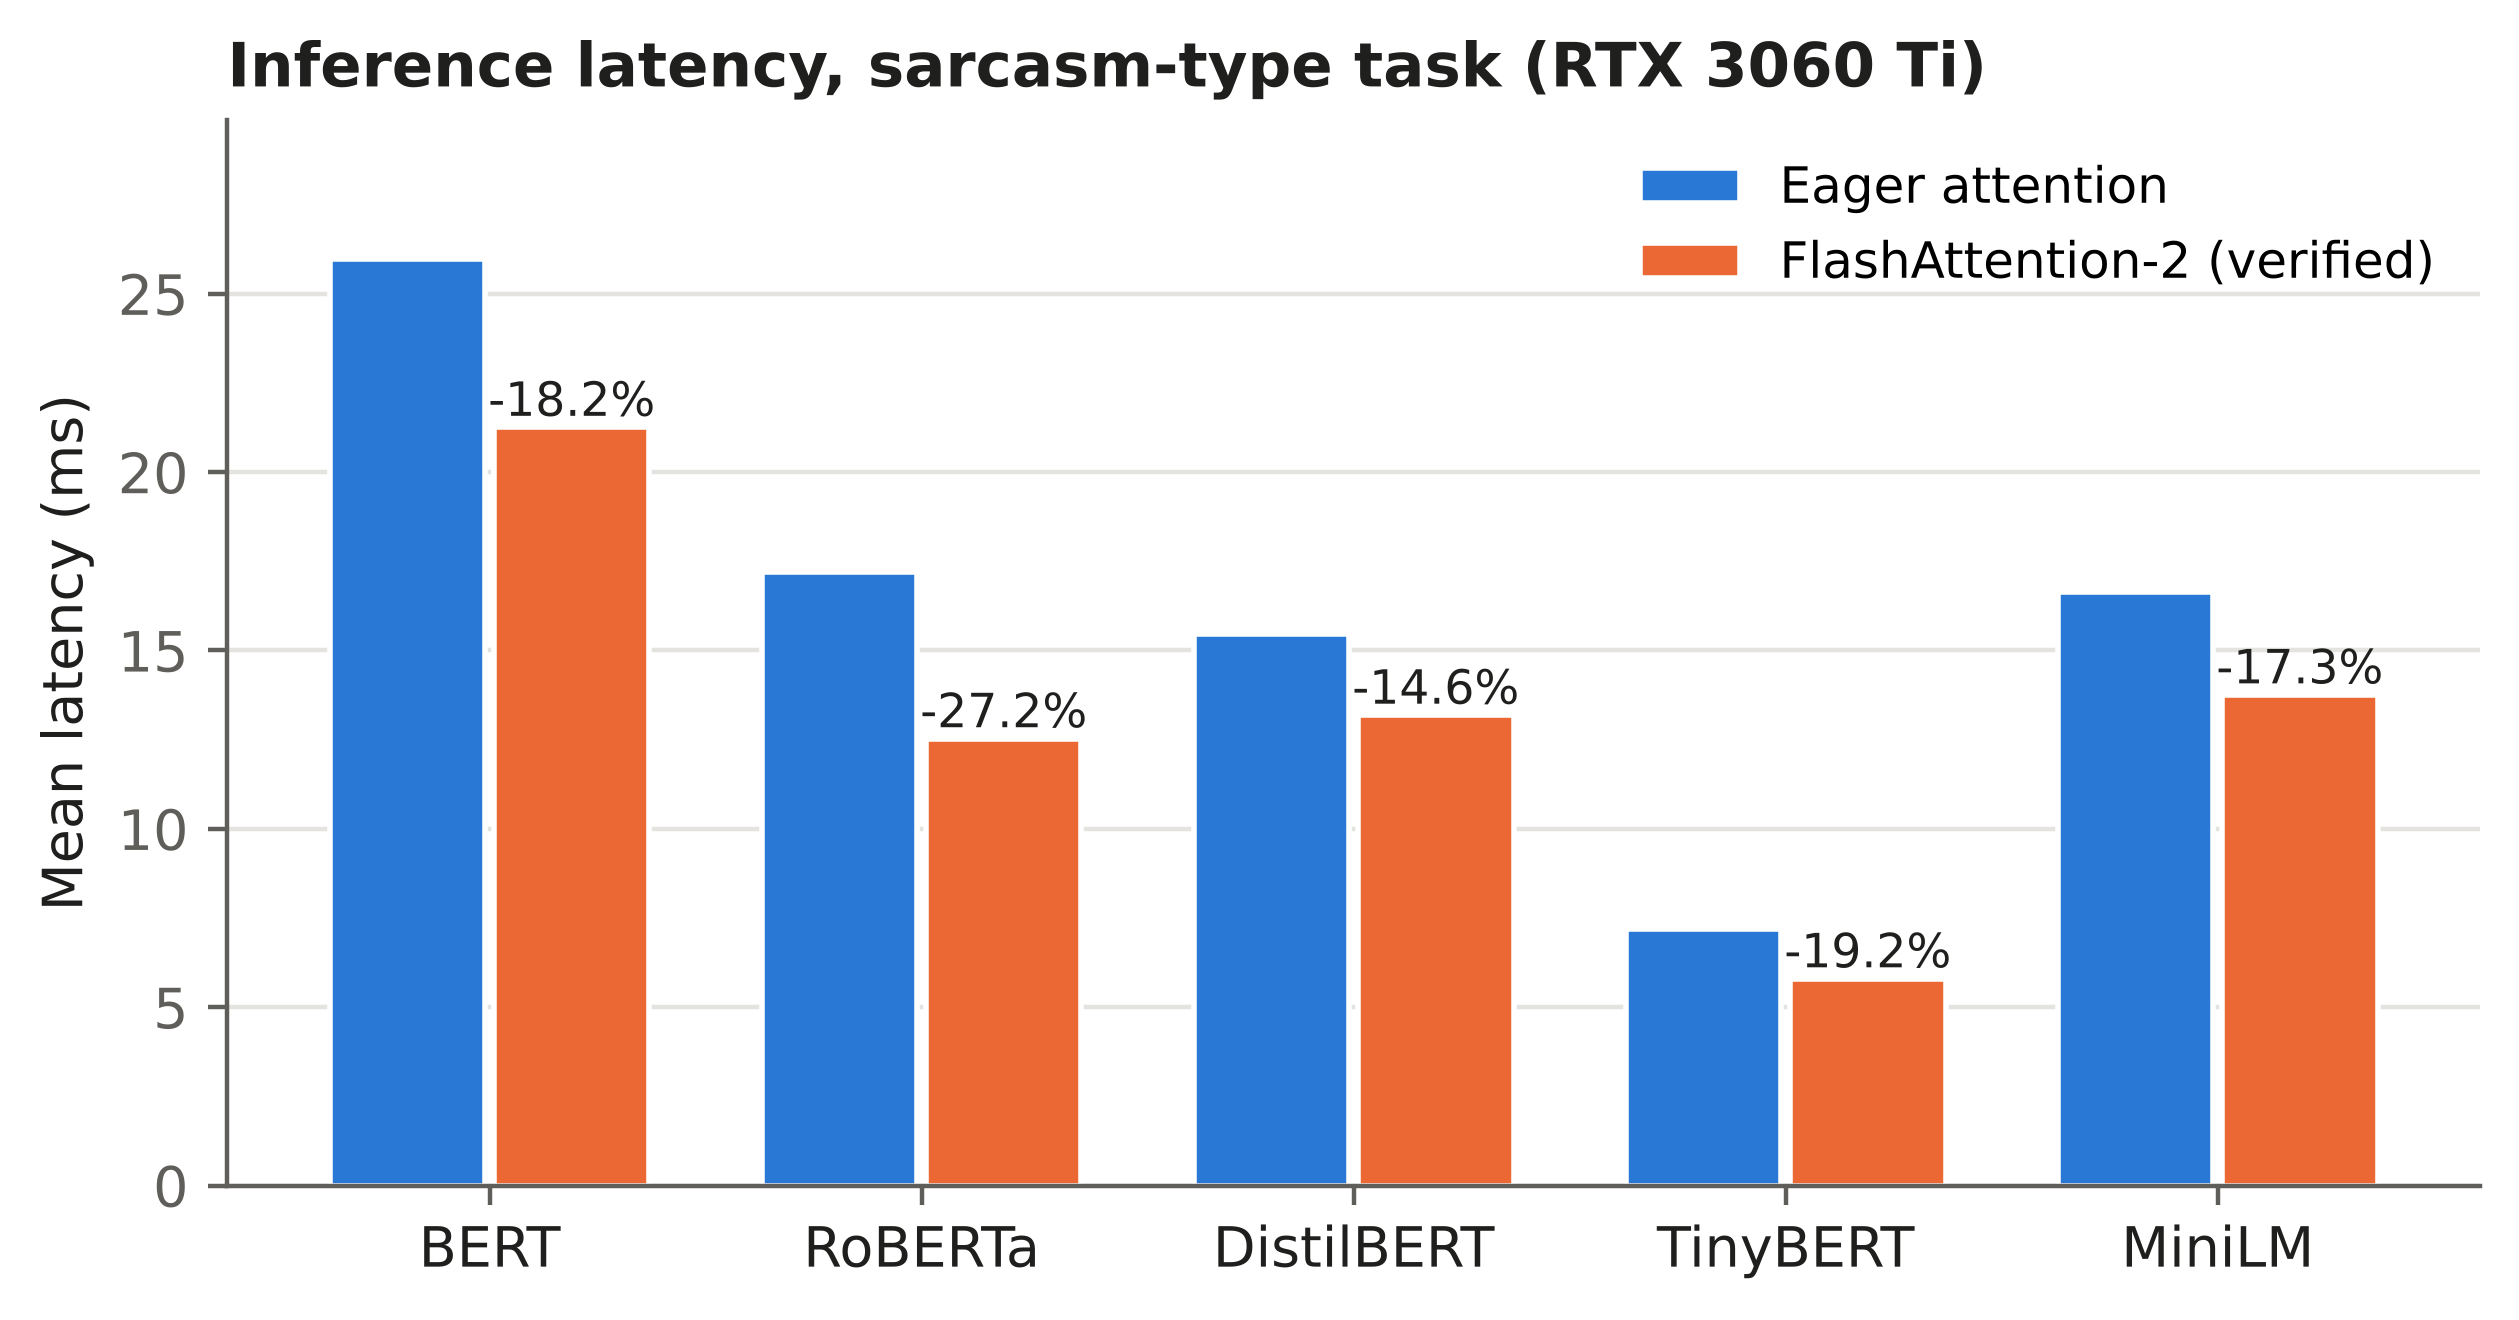
\includegraphics[width=\columnwidth]{fig8_fa_latency.png}
\caption{Mean inference latency under eager attention and verified FlashAttention-2 on the sarcasm-type task.\rcx{R7C7}{ Labels give the change relative to eager attention.}}
\label{fig:fa-latency}
\end{figure}

\subsubsection{Efficiency on the binary task}
\label{sec:efficiency-binary}
\rcrep{R5C11}{Table 11}{Table~\ref{tab:fa-binary}} reports the binary comparison executed on the A100 device. Peak allocated GPU training memory was also recorded in the binary experiment, and it is reported here because it does not follow the pattern observed on the sarcasm-type task. Under the PyTorch scaled dot-product attention backend, peak training memory is unchanged to within measurement resolution for BERT (2575.0 MB in both conditions), MiniLM (2561.2 against 2561.1 MB), TinyBERT (2220.4 against 2220.3 MB) and RoBERTa (2864.3 MB in both conditions), and it increases for DistilBERT, from 2722.8 to 3206.5 MB. We report this rather than presenting only the favourable memory result from the sarcasm-type experiment. The most plausible reading is that the memory benefit observed with the FlashAttention-2 library on the sarcasm-type task does not transfer to the scaled dot-product attention backend used here, and we therefore restrict the memory claim in this manuscript to the experiment in which it was actually observed.

\begin{table}[t]
\caption{Verified FlashAttention comparison on the binary task. \rce{The} optimized condition uses the PyTorch scaled dot-product attention FlashAttention backend; \rce{the} baseline condition uses eager attention. NVIDIA A100-SXM4-40GB (compute capability 8.0), PyTorch 2.6.0, CUDA 12.4, three seeds, mean values. RoBERTa is excluded for the reason stated in the text.}
\label{tab:fa-binary}
\centering\small
\begin{adjustbox}{max width=\textwidth}
\begin{tabular}{lcccccc}
\toprule
 & \multicolumn{2}{c}{Macro F1} & \multicolumn{2}{c}{Training time (s)} & \multicolumn{2}{c}{Latency (ms)} \\
\cmidrule(lr){2-3}\cmidrule(lr){4-5}\cmidrule(lr){6-7}
Model & Eager & Flash & Eager & Flash & Eager & Flash \\
\midrule
BERT & 0.9926 & 0.9911 & 1107.50 & 945.30 ($-$14.6\%) & 13.97 & 11.67 ($-$16.5\%) \\
DistilBERT & 0.9933 & 0.9948 & 550.23 & 450.69 ($-$18.1\%) & 7.50 & 6.32 ($-$15.7\%) \\
TinyBERT & 0.9923 & 0.9914 & 391.57 & 370.34 ($-$5.4\%) & 5.36 & 5.18 ($-$3.4\%) \\
MiniLM & 0.9812 & 0.9867 & 1053.80 & 893.51 ($-$15.2\%) & 14.65 & 12.81 ($-$12.6\%) \\
\bottomrule
\end{tabular}
\end{adjustbox}
\end{table}

RoBERTa is deliberately omitted from \rcrep{R5C11}{Table 11}{Table~\ref{tab:fa-binary}}. In the binary FlashAttention experiment, RoBERTa produced a Macro F1-score of exactly 0.3954 in four of its six runs, comprising the eager runs for seeds 42 and 123 and the FlashAttention runs for seeds 123 and 2024. This value is the arithmetic signature of a classifier that assigns every test review to a single class, and it indicates that fine-tuning failed to converge in those runs rather than that FlashAttention degraded the model. The two runs that did converge reached Macro F1-scores of 0.8880 under eager attention and 0.8415 under the FlashAttention backend, which are themselves well below the 0.9889 obtained by RoBERTa under the main experimental configuration reported in \rcrep{R5C11}{Section 6}{Section~\ref{sec:rq1}}, so the instability affects the magnitude as well as the reliability of the result. The resulting mean of 0.5441 with a standard deviation of 0.2575 for the FlashAttention condition is an average over failed optimization runs and is not a meaningful estimate of model performance. We report this instability explicitly rather than omitting it silently, because it is a genuine and reproducible property of RoBERTa fine-tuning at the batch size and learning rate used in that experiment. The RoBERTa binary efficiency comparison is consequently listed among the open items in the study, and the RoBERTa results reported in \rcrep{R5C11}{Section 6}{Section~\ref{sec:rq1}}, which were obtained under the main experimental configuration and converged on all three seeds, are unaffected by this issue.

\begin{keyfinding}{Key Finding 3}\label{box:kf3}
The verified FlashAttention experiments support a clear and narrowly scoped conclusion. FlashAttention reduces training time by between 11.3\% and 21.9\% on the sarcasm-type task and by between 5.4\% and 18.1\% on the binary task, and reduces mean inference latency by between 14.6\% and 27.2\% on the sarcasm-type task and between 3.4\% and 16.5\% on the binary task. The reductions in training time and latency are consistent in direction across every model and both tasks.

The memory result is not consistent across the two experiments, and we report the difference rather than generalizing from the favourable case. Peak allocated GPU training memory falls by between 10.2\% and 18.1\% on the sarcasm-type task, which uses the FlashAttention-2 library, but is unchanged to within measurement resolution on the binary task, which uses the PyTorch scaled dot-product attention FlashAttention backend, and increases for DistilBERT in that experiment. The memory benefit of FlashAttention therefore appears to depend on the specific implementation rather than on the algorithmic principle alone, and we confine the claim to the experiment in which it was observed.

The effect on predictive performance is different in character and must not be conflated with the efficiency result. On the sarcasm-type task, the Macro F1-score decreases slightly for BERT, RoBERTa, TinyBERT, and MiniLM and increases slightly for DistilBERT, with the largest single change being a decrease of 0.0117 for RoBERTa. On the binary task, the score decreases slightly for BERT and TinyBERT and increases slightly for DistilBERT and MiniLM. These changes are of the same order as the seed-to-seed standard deviations reported in \rcrep{R5C11}{Tables 6 and 8}{Tables~\ref{tab:bin-agg} and~\ref{tab:type-agg}} and are therefore not interpretable as systematic effects of the attention backend. We therefore conclude that FlashAttention reduces computational cost while maintaining comparable predictive performance on both tasks. We make no claim that it improves accuracy, and we have reported the direction and magnitude of every observed predictive change rather than describing the effect only in aggregate.

The pattern of benefit across architectures is also worth noting. RoBERTa\rcdel{R7C4}{, which uses the smallest batch size and consequently performs the largest number of attention operations per epoch,} shows the largest relative gains on the sarcasm-type task, whereas TinyBERT on the binary task shows the smallest gains because its four-layer architecture spends proportionally less of its runtime inside the attention computation. \rcnote{R7C4}{the deleted explanation contradicted Table~\ref{tab:hyper}, which gives the same batch size for every model} This is consistent with the mechanism by which FlashAttention operates, namely the reduction of memory movement within attention rather than the reduction of the total parameter count.
\end{keyfinding}

\subsection{\texorpdfstring{\rcx{R5C9,R7C2,R7C6}{Robustness of the Predictive Results}}{Robustness of the Predictive Results}}
\label{sec:robust}
\rc{R5C9,R7C2,R7C6}{This section examines two threats to the predictive results of Sections~\ref{sec:rq1} to~\ref{sec:stats}, namely the duplicated and conflicting annotations of the released benchmark and the possibility that the high binary scores reflect dataset-specific shortcuts rather than contextual modelling.}

\subsubsection{\texorpdfstring{\rcx{R5C9,R7C2}{Repeated Experiments on Deduplicated Data}}{Repeated Experiments on Deduplicated Data}}
\label{sec:robust-dedup}
\begin{rcblock}{R5C9,R7C2}
All five encoders were fine-tuned again under Protocol B with the hyperparameters of Table~\ref{tab:hyper} and the same three seeds, using the implementation and hardware described in Section~\ref{sec:environment}, and Table~\ref{tab:dedup-results} reports the results together with the change in mean Macro F1 relative to Protocol A. On the binary task the mean Macro F1-score increased for every architecture, by between 0.0024 and 0.0098, and BERT obtains the highest mean Macro F1-score of 0.9975. On the sarcasm-type task the mean Macro F1-score also increased for every architecture, by between 0.1036 and 0.1679, and DistilBERT obtains the highest mean Macro F1-score of 0.9364, followed by BERT at 0.9337 and MiniLM at 0.9318. TinyBERT remains the weakest architecture on both tasks, with mean Macro F1-scores of 0.9872 and 0.8737.

After Holm correction over the sixty paired comparisons of the Protocol B runs, 13 of the 24 comparisons involving TinyBERT remain significant. These are 9 of its 12 comparisons on the sarcasm-type task, including all three seeds against DistilBERT and against MiniLM, but only 4 of its 12 comparisons on the binary task, where every architecture reaches a mean Macro F1-score above 0.987 and the margins are correspondingly small. Among the 36 comparisons between BERT, RoBERTa, DistilBERT and MiniLM, 3 are significant before correction and one remains significant after it, namely RoBERTa against DistilBERT on the sarcasm-type task at seed 2024, with an adjusted $p$-value of 0.024. This difference appears at a single seed, at which RoBERTa produced its weakest run with a Macro F1-score of 0.8734 against 0.9301 and 0.9500 at the other two seeds, so it reflects the instability of RoBERTa rather than a reproducible ranking. The conclusion of Section~\ref{sec:stats} is therefore unchanged, because the ordering of the four stronger architectures is not reproducible across random initializations and TinyBERT is the weakest architecture under both protocols.

The results support two further conclusions. First, the repeated reviews did not inflate the scores of Protocol A, since no review text is shared between partitions under Protocol B and, on the binary task, where the overlapping test reviews of Protocol A were same-label pairs amounting to less than 1\% of the test partition, removing them lowered no score. Second, the large gain on the sarcasm-type task comes mainly from the data rather than from the change of implementation. The lexical baseline of Section~\ref{sec:baselines} is computed in exactly the same way under both protocols and therefore isolates the effect of the data, and its Macro F1-score rises from 0.7425 to 0.8390, a gain of 0.0965 that is close to the gains of the encoders, which lie between 0.1036 and 0.1679. Most of the improvement therefore comes from removing the 230 texts that carry two different sarcasm types, which a single-label classifier cannot predict correctly, and the remainder may reflect the differences of implementation and hardware noted in Section~\ref{sec:environment}. The Protocol B scores on the sarcasm-type task should accordingly be read as performance on reviews with a single agreed sarcasm type, and the Protocol A scores as performance on the benchmark as released, including its label ambiguity.
\end{rcblock}

\begin{table*}[t]
\caption{\rcx{R5C9,R7C2}{Results under Protocol B (deduplicated before partitioning), eager attention, mean and standard deviation over three seeds. $\Delta$ is the change in mean Macro F1 relative to Protocol A (Tables~\ref{tab:bin-agg} and~\ref{tab:type-agg}). Test partitions contain 1,489 binary and 442 sarcasm-type reviews.}}
\rcmark{R5C9,R7C2}
\label{tab:dedup-results}
\centering\small
\iftracked\color{rvBoth}\fi
\begin{adjustbox}{max width=\textwidth}
\begin{tabular}{lccccccc}
\toprule
 & \multicolumn{3}{c}{Binary task} & \multicolumn{4}{c}{Sarcasm-type task} \\
\cmidrule(lr){2-4}\cmidrule(lr){5-8}
Model & Accuracy & Macro F1 & $\Delta$ & Accuracy & Macro F1 & Weighted F1 & $\Delta$ \\
\midrule
BERT & 0.9978 $\pm$ 0.0010 & 0.9975 $\pm$ 0.0011 & $+$0.0034 & 0.9578 $\pm$ 0.0094 & 0.9337 $\pm$ 0.0173 & 0.9579 $\pm$ 0.0091 & $+$0.1036 \\
RoBERTa & 0.9962 $\pm$ 0.0010 & 0.9958 $\pm$ 0.0011 & $+$0.0069 & 0.9487 $\pm$ 0.0232 & 0.9178 $\pm$ 0.0398 & 0.9491 $\pm$ 0.0228 & $+$0.1100 \\
DistilBERT & 0.9969 $\pm$ 0.0019 & 0.9965 $\pm$ 0.0021 & $+$0.0024 & 0.9608 $\pm$ 0.0035 & 0.9364 $\pm$ 0.0055 & 0.9607 $\pm$ 0.0034 & $+$0.1091 \\
TinyBERT & 0.9884 $\pm$ 0.0014 & 0.9872 $\pm$ 0.0015 & $+$0.0098 & 0.9133 $\pm$ 0.0176 & 0.8737 $\pm$ 0.0248 & 0.9138 $\pm$ 0.0174 & $+$0.1679 \\
MiniLM & 0.9957 $\pm$ 0.0017 & 0.9953 $\pm$ 0.0019 & $+$0.0042 & 0.9555 $\pm$ 0.0145 & 0.9318 $\pm$ 0.0240 & 0.9560 $\pm$ 0.0141 & $+$0.1226 \\
\bottomrule
\end{tabular}
\end{adjustbox}
\end{table*}

\subsubsection{\texorpdfstring{\rcx{R7C6}{Lexical and Surface-Feature Baselines}}{Lexical and Surface-Feature Baselines}}
\label{sec:baselines}
\begin{rcblock}{R7C6}
To test whether the high binary scores could be obtained without contextual modelling, we trained three reference models on exactly the partitions of both protocols: a majority-class predictor; a logistic regression on nine surface features that capture review length, word count, exclamation and question marks, capitalization, non-ASCII characters such as emojis, full stops, quotation marks and digits; and a logistic regression on TF-IDF features of word unigrams and bigrams with balanced class weights. Table~\ref{tab:baselines} reports the results.

The surface-feature model reaches a Macro F1-score of only 0.5297 on the binary task and 0.2765 on the sarcasm-type task under Protocol A, so review length, punctuation, capitalization and emoji use do not by themselves separate the classes. The TF-IDF model, by contrast, reaches 0.9673 on the binary task under Protocol A and 0.9719 under Protocol B, which shows that the binary class boundary of this benchmark is largely lexical. The n-grams with the largest weights towards the sarcastic class are intensified evaluative words such as \textit{fun}, \textit{amazing}, \textit{worst}, \textit{awesome}, \textit{terrible}, \textit{funny} and \textit{trash}, whereas moderate evaluative words such as \textit{good}, \textit{nice}, \textit{best} and \textit{cool} carry the largest weights towards the non-sarcastic class, so that in this benchmark extreme praise and extreme condemnation are strong indicators of the sarcastic label. The fine-tuned encoders improve on the lexical model by about 2.7 Macro F1 points on the binary task and by about 8.8 points on the sarcasm-type task under Protocol A (0.8301 against 0.7425), which means that the contribution of contextual encoding is modest on the binary task and substantial on the fine-grained task. The margins are similar under Protocol B, at 2.6 points on the binary task (0.9975 against 0.9719) and 9.7 points on the sarcasm-type task (0.9364 against 0.8390).

The benchmark does not record the source application of the annotated reviews, so we cannot test whether part of this lexical signal is application-specific, for example whether reviews of deliberately humorous applications are predominantly labelled sarcastic, and Section~\ref{sec:threats} discusses this limitation.
\end{rcblock}

\begin{table}[t]
\caption{\rcx{R7C6}{Lexical and surface-feature baselines on the partitions of both protocols, mean and standard deviation of Macro F1 over three seeds. The fine-tuned encoders reach 0.9941 (binary) and 0.8301 (sarcasm type) under Protocol A.}}
\rcmark{R7C6}
\label{tab:baselines}
\centering\small
\iftracked\color{rvSeven}\fi
\begin{adjustbox}{max width=\textwidth}
\begin{tabular}{lcccc}
\toprule
 & \multicolumn{2}{c}{Binary task} & \multicolumn{2}{c}{Sarcasm-type task} \\
\cmidrule(lr){2-3}\cmidrule(lr){4-5}
Model & Protocol A & Protocol B & Protocol A & Protocol B \\
\midrule
Majority class & 0.3954 $\pm$ 0.0000 & 0.3947 $\pm$ 0.0000 & 0.1324 $\pm$ 0.0002 & 0.1385 $\pm$ 0.0000 \\
Surface features + LR & 0.5297 $\pm$ 0.0027 & 0.5201 $\pm$ 0.0074 & 0.2765 $\pm$ 0.0074 & 0.2959 $\pm$ 0.0166 \\
TF-IDF + LR & 0.9673 $\pm$ 0.0023 & 0.9719 $\pm$ 0.0032 & 0.7425 $\pm$ 0.0022 & 0.8390 $\pm$ 0.0054 \\
\bottomrule
\end{tabular}
\end{adjustbox}
\end{table}

\subsection{\texorpdfstring{\rcx{R7C3}{Validation of Confidence-Based Routing}}{Validation of Confidence-Based Routing}}
\label{sec:routing}
\begin{rcblock}{R7C3}
The routing stage of Section~\ref{sec:pipeline-method} is useful only if its confidence score separates reliable from unreliable predictions. We evaluated this on the Protocol B test partitions, using for each task the architecture with the highest mean validation Macro F1-score, as prescribed by Algorithm~\ref{alg:workflow}, which is BERT for the binary task and DistilBERT for the sarcasm-type task. Calibration is reported as the mean over the three seeds, whereas the threshold sweep and the second-opinion analysis pool the three test partitions, which contain 4,467 binary and 1,326 sarcasm-type reviews in total, because only a handful of test reviews fall below the threshold in any one seed.

\textit{Calibration.} The expected calibration error of Equation~\eqref{eq:ece} is 0.0019 on the binary task and 0.0216 on the sarcasm-type task, so the confidence scores of the fine-tuned models are already well calibrated. Temperature scaling fitted on the validation partition, with fitted temperatures of 1.42 and 1.19, does not improve them further, and the error becomes 0.0033 and 0.0220 respectively. Since temperature scaling would change no predicted label and does not reduce the calibration error, the pipeline thresholds the uncalibrated confidence scores.

\textit{Threshold sweep.} Table~\ref{tab:routing} reports, for thresholds between 0.5 and 0.9, the number of routed reviews, the accuracy of the accepted and of the routed predictions, and the number of misclassifications that fall in the routed set, and it shows that the two tasks behave very differently. On the binary task the model is almost never uncertain, because at $\tau = 0.7$ only 4 of the 4,467 test reviews (0.09\%) are routed and all four are classified correctly; the model makes 10 errors in total, 9 of them with a confidence of at least 0.98, so no threshold in the range examined captures more than one of them. On the sarcasm-type task the confidence score is informative. At $\tau = 0.7$, 16 test reviews (1.21\%) are routed and their accuracy is 0.6250, against 0.9649 for the accepted predictions, and raising the threshold to 0.9 routes 51 reviews (3.85\%) and raises the accuracy of the accepted predictions to 0.9718. Routing nevertheless captures only a minority of the errors, 6 of 52 at $\tau = 0.7$ and 16 of 52 at $\tau = 0.9$, because most misclassifications are made with high confidence. This is the setting of selective classification \citep{geifman2017selective}, in which a model abstains on inputs whose confidence is low, and the results show both its value and its limits here: confidence-based routing identifies a small set of reviews that deserve human attention, particularly on the fine-grained task, but it does not detect most of the errors of a highly confident model. We retain $\tau = 0.7$ as the operating point used throughout the manuscript, and Table~\ref{tab:routing} allows a practitioner to choose a different point according to the review capacity available.

\textit{Independent second opinion.} Because the deployed secondary stage re-applies the same model, it cannot correct predictions. To quantify what an independent secondary stage would contribute, we replaced the label of every routed review with the arg max of the averaged probabilities of the other fine-tuned encoders, excluding TinyBERT because of its lower performance. On the binary task this changes nothing, since the four routed reviews were already classified correctly. On the sarcasm-type task the accuracy on the routed reviews rises from 0.6250 to 0.6875, because across the three seeds the second opinion corrects 5 predictions and introduces 4 new errors, and the mean Macro F1-score over the whole test partition changes from 0.9364 to 0.9391. The benefit of an independent second opinion is therefore small and limited by the small number of routed reviews, and the deployed configuration retains the same-model secondary stage for triage.
\end{rcblock}

\begin{table*}[t]
\caption{\rcx{R7C3}{Threshold sweep for confidence-based routing on the Protocol B test partitions, with the three seeds pooled. Routed gives the number and percentage of test reviews whose confidence falls below $\tau$; accuracy is reported separately for accepted and routed predictions; Errors routed gives how many of the misclassifications of the model fall in the routed set. The architecture used for each task and the number of pooled test reviews are given in the header, and n/a indicates that no review is routed.}}
\rcmark{R7C3}
\label{tab:routing}
\centering\small
\iftracked\color{rvSeven}\fi
\begin{adjustbox}{max width=\textwidth}
\begin{tabular}{ccccccccc}
\toprule
 & \multicolumn{4}{c}{Binary task (BERT, 4,467 reviews)} & \multicolumn{4}{c}{Sarcasm-type task (DistilBERT, 1,326 reviews)} \\
\cmidrule(lr){2-5}\cmidrule(lr){6-9}
$\tau$ & Routed, $n$ (\%) & Acc.\ accepted & Acc.\ routed & Errors routed & Routed, $n$ (\%) & Acc.\ accepted & Acc.\ routed & Errors routed \\
\midrule
0.5 & 0 (0.00) & 0.9978 & n/a & 0 of 10 & 4 (0.30) & 0.9622 & 0.5000 & 2 of 52 \\
0.6 & 1 (0.02) & 0.9978 & 1.0000 & 0 of 10 & 13 (0.98) & 0.9650 & 0.5385 & 6 of 52 \\
0.7 & 4 (0.09) & 0.9978 & 1.0000 & 0 of 10 & 16 (1.21) & 0.9649 & 0.6250 & 6 of 52 \\
0.8 & 5 (0.11) & 0.9980 & 0.8000 & 1 of 10 & 31 (2.34) & 0.9683 & 0.6452 & 11 of 52 \\
0.9 & 5 (0.11) & 0.9980 & 0.8000 & 1 of 10 & 51 (3.85) & 0.9718 & 0.6863 & 16 of 52 \\
\bottomrule
\end{tabular}
\end{adjustbox}
\end{table*}

\subsection{Comparison with an Instruction-Tuned Large Language Model}
\label{sec:llm}
The previous version of this manuscript positioned the work relative to instruction-tuned large language models without providing an empirical comparison. To address this gap, we evaluated Mistral-7B-Instruct-v0.3 in a zero-shot configuration on both tasks using the identical\rc{R5C9,R7C2}{ Protocol A} test partitions and the identical three random seeds. The model was loaded with four-bit quantization, the maximum input length was 512 tokens, and generation was limited to ten new tokens. Predictions were parsed from the generated text and mapped to the label space, and all 1,500 binary outputs and all sarcasm-type outputs were parsed successfully, so the results are not affected by output-format failures. \rcrep{R5C11}{Table 12}{Table~\ref{tab:llm}} reports the comparison.

\begin{table}[t]
\caption{Zero-shot instruction-tuned large language model compared with the fine-tuned encoder architectures\rcx{R5C9,R7C2}{ under Protocol A}. Encoder values are the best performing \rce{models} per task from \rcrep{R5C11}{Tables 6 and 8}{Tables~\ref{tab:bin-agg} and~\ref{tab:type-agg}}.}
\label{tab:llm}
\centering\small
\begin{adjustbox}{max width=\textwidth}
\begin{tabular}{lllcc}
\toprule
Task & Model & Setting & Accuracy & Macro F1 \\
\midrule
Binary & BERT & fine-tuned & 0.9947 $\pm$ 0.0018 & 0.9941 $\pm$ 0.0020 \\
Binary & DistilBERT & fine-tuned & 0.9947 $\pm$ 0.0007 & 0.9941 $\pm$ 0.0007 \\
Binary & Mistral-7B-Instruct-v0.3 & zero-shot & 0.3596 $\pm$ 0.0052 & 0.3110 $\pm$ 0.0055 \\
\midrule
Sarcasm type & BERT & fine-tuned & 0.8690 $\pm$ 0.0051 & 0.8301 $\pm$ 0.0072 \\
Sarcasm type & DistilBERT & fine-tuned & 0.8696 $\pm$ 0.0080 & 0.8273 $\pm$ 0.0194 \\
Sarcasm type & Mistral-7B-Instruct-v0.3 & zero-shot & 0.2415 $\pm$ 0.0125 & 0.1664 $\pm$ 0.0101 \\
\bottomrule
\end{tabular}
\end{adjustbox}
\end{table}

The zero-shot model performs substantially below every fine-tuned encoder, and on the binary task its accuracy of 0.3596 is below the majority-class rate of 0.654. Inspection of the stored predictions identifies the cause. The model assigns the sarcastic label to 1,393 of the 1,500 binary test reviews, which produces high recall on the minority class at the cost of a very large number of false positives. Mean inference latency was 433 ms per review for the binary task and 576 ms for the sarcasm-type task, compared with between 5 and 26 ms for the fine-tuned encoders.

This comparison must be interpreted with care, and we state its limits explicitly. It evaluates a single instruction-tuned model, in a single zero-shot prompt formulation, under four-bit quantization, without few-shot exemplars, without prompt optimization, and without task-specific fine-tuning. It therefore establishes that an unadapted instruction-tuned model is not competitive with a fine-tuned encoder on this task and this dataset, and it does not establish any general claim about the capability of large language models for sarcasm detection. A parameter-efficient fine-tuned large language model, or the same model with a calibrated prompt and few-shot exemplars, could plausibly perform very differently, and we identify this as future work. Within these limits, the result supports the design rationale of the present framework, namely that compact fine-tuned encoders offer a more favourable balance of predictive performance and inference cost for \rcrep{R5C1,R7C5}{continuous app-review analytics}{app-review analytics that runs repeatedly}.

\subsection{Comparative Analysis with Existing Approaches}
\label{sec:comparison}
To assess the contribution of the proposed framework relative to prior work, we compare it with representative sarcasm detection studies. The comparison considers the application domain, the modelling strategy, the classification task, the evaluation protocol, and the deployment characteristics. \rcrep{R5C11}{Table 13}{Table~\ref{tab:comparison}} summarizes the comparison and distinguishes explicitly between values reported in the source literature and values measured experimentally in the present study.

\begin{table*}[t]
\caption{Comparison of the proposed framework with representative sarcasm detection studies. The Result type column distinguishes metrics reported in the source publication from metrics measured experimentally in this study.}
\label{tab:comparison}
\centering\small
\begin{adjustbox}{max width=\textwidth}
\begin{tabular}{p{2.8cm}p{2.3cm}p{2.3cm}p{1.6cm}p{1.4cm}p{3.2cm}p{2.6cm}}
\toprule
Study & Dataset & Best model & Task & Macro F1 & Result type & Deployment features \\
\midrule
\citet{sinha2023sarcasm} & Twitter & Entailment network & Binary & 0.84 & Reported in source & None \\
\citet{kamal2022cat} & Product reviews & CNN + BiGRU & Binary & 0.88 & Reported in source & None \\
\citet{fatima2024exploratory} & Google Play reviews & BiGRU & Sarcasm type & 0.95 & Derived from reported class-wise F1 & None \\
\citet{fatima2024exploratory} & Google Play reviews & CNN & Sarcasm type & 0.94 & Derived from reported class-wise F1 & None \\
This study & Google Play reviews & BERT & Sarcasm type & 0.830 $\pm$ 0.007 & Measured, 3 seeds, held-out test\rc{R5C9,R7C2}{ (Protocol A)} & FlashAttention; confidence-based routing \\
This study & Google Play reviews & BERT / DistilBERT & Binary & 0.994 $\pm$ 0.002 & Measured, 3 seeds, held-out test\rc{R5C9,R7C2}{ (Protocol A)} & FlashAttention; confidence-based routing \\
\bottomrule
\end{tabular}
\end{adjustbox}
\end{table*}

The most closely related study is that of \rcrep{R7C7}{Fatima et al. Fatima et al. (2024)}{\citet{fatima2024exploratory}}, because the present work uses the benchmark corpus introduced in that study. A precise comparison with that work requires care, and we set out the methodological differences before drawing any conclusion.

The two studies differ in four respects that jointly prevent a direct numerical comparison. First, the evaluation protocols differ. Fatima et al. report results obtained under $k$-fold cross-validation applied after data balancing, with five folds for the binary task and ten folds for the sarcasm-type task, so their reported metrics are computed on partitions that include synthetically duplicated minority instances. The present study evaluates on a held-out test partition that was never oversampled, with oversampling confined to the training partition, and repeats the procedure across three random seeds. An evaluation set that contains duplicated minority examples produced by random oversampling is systematically easier than one that preserves the natural class distribution, and metrics obtained under the two protocols are therefore not on a common scale. Second, the model families differ, since Fatima et al. evaluate recurrent and convolutional architectures trained from randomly initialized embeddings, whereas this study fine-tunes pretrained transformer encoders. Third, the source publication reports class-wise F1-scores and overall accuracy rather than Macro F1, so the Macro F1 values shown for that work in \rcrep{R5C11}{Table 13}{Table~\ref{tab:comparison}} were derived by us as the unweighted mean of the reported class-wise F1-scores and are labelled accordingly. Fourth, the studies pursue different objectives, since Fatima et al. establish the dataset and the feasibility of automated sarcasm-type detection, whereas the present study addresses the deployment efficiency of that detection.

Given these differences, we make no claim of superiority over Fatima et al. on the sarcasm-type task. The derived Macro F1 values for the recurrent and convolutional models in that study range from 0.904 to 0.950, which is numerically higher than the 0.830 obtained here, and we attribute this difference primarily to the difference in evaluation protocol rather than to a difference in model capability. The values shown for that study in \rcrep{R5C11}{Table 13}{Table~\ref{tab:comparison}} are literature-reported results, taken from the class-wise F1-scores published in the source article, from which we computed an unweighted mean. We did not re-implement, retrain or otherwise reproduce the experiments of Fatima et al., and no replicated value for that work is presented anywhere in this manuscript. The comparison in \rcrep{R5C11}{Table 13}{Table~\ref{tab:comparison}} should accordingly be read as contextual positioning against published results rather than as a controlled head-to-head experiment, because the two studies differ in evaluation protocol, preprocessing, data partitioning and model family.

The contribution of the present study relative to that baseline is consequently not an improvement in classification accuracy. It consists of an evaluation protocol that reports performance on an unmodified test distribution with repeated seeds, confidence intervals, and paired significance testing\rc{R5C10}{ with correction for multiple comparisons}\rc{R5C9,R7C2}{, together with a replication on data deduplicated before partitioning}; an empirical quantification of the training-time, latency, and GPU-memory effects of verified FlashAttention on this task; an empirical comparison against \rc{R7C6}{lexical baselines and} an instruction-tuned large language model; and a confidence-based routing mechanism that supports \rcrep{R5C1,R7C5}{continuous operation}{scheduled operation\rc{R7C3}{ and whose calibration and threshold behaviour have been measured}}. These are deployment-oriented contributions, and they are complementary to rather than competitive with the contribution of the original benchmark study.

\subsection{Automated Pipeline and Cloud Deployment}
\label{sec:pipeline-results}
The framework is deployed within the automated, confidence-aware orchestration pipeline described in \rcrep{R5C11}{Section 3.7}{Section~\ref{sec:pipeline-method}}. The pipeline supports scheduled data ingestion, sarcasm prediction, confidence-based routing of uncertain predictions, synchronization of aggregated results with a cloud analytics layer, and notification of downstream services such as issue trackers. This provides an automated processing pipeline that can support developer analysis of incoming reviews, rather than an offline classification experiment alone. The pipeline was evaluated on an offline benchmark, and the reported latency indicates that it can support low-latency processing of incoming reviews; we do not claim demonstrated production-grade continuous operation, since no live deployment was benchmarked.

Two properties of this mechanism should be stated precisely. First, the routing step re-evaluates low-confidence predictions using the same fine-tuned model rather than an independent verifier. It therefore modulates which predictions receive additional processing and how they are flagged for human attention, and it does not by itself correct predictions. We describe it as confidence-based routing rather than as verification for this reason. \rcrep{R7C3}{A genuine verification stage would require an independent model, an alternative input view, or an ensemble decision, and its design and evaluation remain future work.}{Section~\ref{sec:routing} shows that its confidence score separates more accurate from less accurate predictions on the sarcasm-type task, that most errors are nevertheless made with high confidence, and that an independent second opinion built from the other encoders would add only a small benefit.} Second, the pipeline executes a predefined sequence of operations with a single confidence-conditioned branch. It does not perform autonomous planning, goal generation, or open-ended tool selection, and the terminology used throughout this manuscript reflects that scope.

The efficiency results reported for RQ3 are directly relevant to this deployment setting. The reductions in inference latency\rcdel{R7C4}{and peak GPU memory} obtained with verified FlashAttention lower the per-review processing cost, which is the dominant recurring cost in a \rcrep{R5C1,R7C5}{continuously operating pipeline}{pipeline that runs repeatedly}, and\rc{R7C4}{, where the FlashAttention-2 library is used,} the reductions in peak training memory lower the hardware requirement for the scheduled offline retraining cycles described in \rcrep{R5C11}{Section 3.7}{Section~\ref{sec:pipeline-method}}.

\begin{keyfinding}{Summary of Results}\label{box:summary}
Fine-tuned transformer encoders detect sarcasm in app reviews with a mean Macro F1-score of up to 0.9941, and classify sarcasm into five types with a mean Macro F1-score of up to 0.8301\rc{R5C9,R7C2}{, on the benchmark as released}. Paired statistical testing\rc{R5C10}{ with Holm correction} establishes that TinyBERT performs significantly worse than \rcrep{R5C10}{the other four architectures on both tasks and that the remaining four architectures are not reliably distinguishable from one another}{BERT and DistilBERT on both tasks and that no difference among BERT, RoBERTa, DistilBERT and MiniLM survives the correction}, which means that model selection for this task can be driven by computational cost. \rc{R5C9,R7C2}{Repeating the experiments on deduplicated data gives best mean Macro F1-scores of 0.9975 and 0.9364, keeps TinyBERT as the weakest architecture and leaves a single significant comparison among the other four at one seed only, with the gain on the sarcasm-type task coming mainly from the removal of reviews that carry conflicting annotations.} \rc{R7C6}{A TF-IDF baseline reaches 0.9673 on the binary task, so the binary boundary of this benchmark is largely lexical, while contextual encoding adds about nine to ten Macro F1 points on the sarcasm-type task.} Verified FlashAttention reduces training time\rcrep{R7C4}{, inference latency, and peak GPU memory consistently across architectures and tasks}{ and inference latency consistently across architectures and tasks, and it reduces peak training memory only with the FlashAttention-2 library,} while leaving predictive performance materially unchanged. \rc{R7C3}{The confidence scores used for routing are already well calibrated and are not improved by temperature scaling, and on the sarcasm-type task routed predictions are far less accurate than accepted ones, although most errors are made with high confidence, so routing flags a small set of uncertain reviews rather than most of the errors.} A zero-shot instruction-tuned large language model is not competitive with the fine-tuned encoders on this dataset under the single prompt configuration evaluated. Taken together, these results support the deployment-oriented framing of the proposed framework rather than a claim of improved classification accuracy over prior work.
\end{keyfinding}

%% ============================================================================
\section{Discussion and Implications}
\label{sec:discussion}
The experimental findings demonstrate that transformer-based architectures are highly effective for sarcasm detection in mobile app reviews, particularly when contextual understanding and implicit sentiment interpretation are required. Across both binary and multi-class settings, the evaluated models consistently achieved strong performance\rcrep{R7C6}{, confirming that self-attention mechanisms are capable of capturing the contrast between literal wording and intended meaning}{, although the comparison with the lexical baseline shows that on the binary task most of the class boundary is already captured by word and bigram statistics, so the advantage of contextual encoding is concentrated in the fine-grained task, where the encoders exceed the lexical baseline by about nine Macro F1 points}. \rcrep{R5C10}{In particular, RoBERTa and BERT showed superior performance due to their deeper contextual representation capabilities, while lightweight architectures such as TinyBERT and MiniLM provided competitive results with substantially lower computational cost.}{The statistical analysis does not support a ranking among BERT, RoBERTa, DistilBERT and MiniLM, and only the deficit of TinyBERT is reproducible across seeds after correction for multiple comparisons, so the compact MiniLM and DistilBERT models deliver the predictive performance of the larger encoders at a substantially lower computational cost.} These observations highlight an important trade-off between predictive accuracy and deployment efficiency in real-world software analytics systems.

A major contribution of this work lies in shifting sarcasm detection beyond a purely accuracy-driven task toward an inference-optimized and deployment-oriented framework. Unlike many previous studies that primarily focus on improving classification scores, this research explicitly investigates computational efficiency and scalability through the integration of FlashAttention. The results demonstrate that FlashAttention \rcrep{R7C4}{significantly reduces training time, inference latency, and memory overhead while maintaining comparable predictive performance across models}{reduces training time and inference latency for every architecture while maintaining comparable predictive performance, and that its memory benefit depends on the implementation, since it appears with the FlashAttention-2 library but not with the PyTorch scaled dot-product attention backend}. This is particularly important in large-scale app-review ecosystems, where millions of reviews may need to be processed \rcrep{R5C1,R7C5}{continuously and in near real time}{repeatedly and with low latency}. The findings therefore suggest that efficiency-aware transformer optimization is essential for practical adoption within industrial software engineering environments.

The study also contributes to the growing intersection between Natural Language Processing and Natural Language-Based Software Engineering (NLbSE). App reviews frequently contain indirect criticism, exaggerated praise, humor, and passive-aggressive expressions that are difficult to interpret using conventional sentiment analysis techniques. By incorporating fine-grained sarcasm categorization, the proposed framework enables deeper understanding of user intent and emotional polarity within software-related feedback. This has important implications for software maintenance and evolution, as developers may otherwise overlook critical usability issues or incorrectly prioritize user requirements due to misleading sentiment signals.

Another implication of this work is the integration of an automated, confidence-aware orchestration pipeline for \rcdel{R5C1,R7C5}{continuous} sarcasm-aware analytics. Rather than functioning as a static offline classifier, the proposed framework operates as an automated decision-support component that ingests reviews on a schedule, routes uncertain predictions for additional processing, and updates cloud-based workflows. \rc{R7C3}{The routing validation shows that the confidence score is informative on the sarcasm-type task, where routed predictions are far less accurate than accepted ones, and it also shows that the fine-tuned models are confident even when they are wrong, so routing should be understood as a way of surfacing a small number of uncertain reviews rather than as a safeguard against most errors.} This design demonstrates how sarcasm detection can be embedded into software analytics pipelines and integrated with external tools such as dashboards, issue-tracking systems, and monitoring services. The orchestration layer therefore extends the applicability of sarcasm detection from a research-oriented classification task to a deployable software analytics component, within the scope defined in \rcrep{R5C11}{Section 3.7}{Section~\ref{sec:pipeline-method}}.

From a broader perspective, the findings indicate that lightweight and efficiency-aware transformer architectures may provide a more practical alternative to large-scale language models for \rcrep{R5C1,R7C5}{continuous software analytics tasks}{software analytics tasks that run repeatedly}. Although modern large language models demonstrate impressive general-purpose reasoning ability, their deployment cost, inference latency, and reproducibility challenges often limit their suitability for scalable industrial environments. The zero-shot comparison reported in \rcrep{R5C11}{Section 6.2}{Section~\ref{sec:llm}} provides direct empirical support for this position on the present dataset, subject to the scope limitations stated there. The combination of compact transformer architectures, verified FlashAttention optimization, and automated orchestration provides a balance between contextual understanding, computational efficiency, and deployment feasibility.

Overall, this study demonstrates that sarcasm-aware sentiment analysis can move beyond isolated NLP experimentation toward scalable and operational software engineering applications. By combining transformer-based contextual modelling, verified inference optimization, repeated-seed statistical validation\rc{R5C10}{ with correction for multiple comparisons}, \rc{R5C9,R7C2}{a deduplicated replication, }\rc{R7C3}{an empirical validation of confidence-based routing, }and automated orchestration, the proposed framework provides practical advances for app-review analytics and software feedback processing.

%% ============================================================================
\section{Threats to Validity}
\label{sec:threats}
Despite the strong empirical performance of the proposed framework, several threats to validity should be considered. Internal validity may be influenced by experimental design choices such as learning rate, batch size, optimizer configuration, and early stopping during fine-tuning. Although all transformer models were trained under identical experimental settings to ensure a fair comparison, alternative hyperparameter configurations could lead to different performance outcomes. In addition, FlashAttention operates at the GPU kernel level, and its computational efficiency may vary depending on hardware characteristics, including GPU architecture, CUDA version, and memory bandwidth. Consequently, execution-time improvements may differ across deployment platforms.

The experiments were conducted using a publicly available benchmark dataset with stratified training, validation, and test partitions. \rcrep{R5C9,R7C2}{A duplicate-text audit of the partitions identified a small number of reviews whose exact text appears in more than one partition, amounting to between five and eleven training and test pairs per seed for the binary task and between forty-eight and fifty-four per seed for the sarcasm-type task. These overlaps originate in the benchmark corpus itself, which contains 82 duplicated rows in the binary dataset and 487 duplicated rows in the sarcasm-type dataset. For the sarcasm-type task, the affected instances correspond to approximately two percent of a training partition of 2,422 reviews, and the resulting optimistic bias is therefore expected to be small but is not zero. We report these counts explicitly rather than omitting them, and deduplication prior to partitioning is identified as a necessary refinement of the protocol.}{The released benchmark contains repeated reviews and reviews annotated with conflicting sarcasm types (Section~\ref{sec:duplicates}). Under Protocol A, between 13 and 14 binary test reviews per seed occur in training with the same label and between 9 and 15 sarcasm-type test reviews per seed do so, while a further 45 to 52 sarcasm-type test reviews occur in training only under a different label, which can lower but not inflate the scores. We therefore repeated all encoder experiments under Protocol B, in which the data are deduplicated before partitioning, and both sets of results are reported. Because the Protocol B runs used a training script written for this revision and different hardware, a difference between the two protocols combines the effect of deduplication with any effect of implementation, although the lexical baseline, computed identically under both protocols, indicates that the change of data accounts for most of the difference on the sarcasm-type task.} In addition, because the benchmark dataset does not provide complete user-level \rc{R7C6}{or application-level} metadata, it is not possible to verify whether multiple reviews written by the same user appear across partitions. Similarly, reviews originating from the same application may exist in both subsets as part of the original benchmark construction. Although this experimental protocol follows the benchmark dataset and previous studies, future work should investigate user-level and application-level partitioning strategies to further reduce the possibility of information leakage and evaluate cross-application generalization more rigorously.

Construct validity is constrained by the subjective nature of sarcasm, which frequently depends on contextual, cultural, pragmatic, and discourse-level cues that cannot always be fully captured through textual information alone. While the benchmark dataset follows established annotation guidelines, ambiguity between closely related categories (\rce{for example} Humor and Irony) may introduce labeling uncertainty, particularly in fine-grained multi-class classification. \rc{R5C9,R7C2}{The audit of Section~\ref{sec:duplicates} confirms this uncertainty, since 230 texts in the sarcasm-type file carry two or more different types, most often pairs involving Self-Deprecation, Humor and Irony.} \rc{R5C8,R7C1}{In this benchmark the Self-Deprecation category consists mainly of exaggerated mock condemnation by or about an application rather than the narrower linguistic sense of a speaker who mocks themselves, and results for this category should be read with that operational meaning in mind.} \rc{R5C9,R7C2}{The sarcasm-type file is also not a strict subset of the sarcastic reviews of the binary file, since 253 of its reviews are labelled non-sarcastic in the binary file and 106 have no counterpart there; this affects no reported metric, but a cascaded deployment that applies the type classifier only to reviews flagged by the binary classifier would encounter a slightly different distribution of types than the one evaluated here.} Furthermore, the sarcasm taxonomy adopted in this study is limited to the categories available in the benchmark dataset. Although the proposed framework supports fine-grained sarcasm classification, the current evaluation focuses on five sarcasm categories, namely Humor, Irony, Flattery, Passive Aggression, and Self-Deprecation. Other linguistically important forms, including hyperbolic sarcasm, rhetorical sarcasm, dropped-negation sarcasm, oxymoronic sarcasm, and deadpan sarcasm, are not explicitly represented in the training corpus. Consequently, the proposed framework may exhibit reduced generalization when encountering sarcasm expressions that differ substantially from those represented in the benchmark dataset. Because this work employs a publicly available benchmark corpus, detailed demographic information regarding the original annotators is unavailable. Therefore, the potential influence of annotator background, cultural experience, linguistic preferences, or demographic characteristics on sarcasm interpretation cannot be fully assessed. Since sarcasm perception is inherently subjective, these factors may introduce systematic labeling bias that influences both model training and evaluation. Future benchmark datasets reporting detailed annotation protocols and annotator characteristics would enable a more comprehensive assessment of these effects.

Another limitation concerns the robustness of the proposed framework when processing noisy or adversarial user-generated content. Although the benchmark dataset naturally contains variations in writing style, spelling, punctuation, and informal language, the present study does not explicitly evaluate robustness against adversarial text perturbations, such as intentional misspellings, character substitutions, excessive punctuation, emoji insertion, or lexical modifications designed to alter model predictions. Likewise, certain sarcastic expressions depend heavily on conversational history, shared background knowledge, cultural context, or implicit pragmatic cues that may not be fully represented in isolated review text. Consequently, although the proposed framework demonstrates strong performance on the benchmark dataset, its robustness under adversarial or highly ambiguous real-world conditions remains an open research challenge. Future work will investigate adversarial robustness, data augmentation strategies, robust transformer training, and context-aware reasoning mechanisms to improve resilience against noisy, manipulated, and highly contextual software reviews.

External validity is constrained by the use of Google Play Store reviews collected from seven mobile applications, which may not fully represent sarcasm patterns occurring in other software engineering environments, social media platforms, online forums, customer-support conversations, or multilingual communication settings. Sarcasm frequently depends on cultural background, regional language variation, community-specific conventions, and application context. Consequently, the reported findings should not be assumed to generalize directly across different domains or languages. Future work should therefore evaluate the proposed framework on multilingual datasets, cross-domain software feedback, conversational corpora, and multimodal sarcasm datasets while incorporating richer contextual information, conversational history, user-behavior modeling, and discourse-aware reasoning. Another limitation is that the experimental evaluation focuses primarily on inference-optimized encoder-based transformer architectures rather than instruction-tuned generative large language models. This design choice is intentional and consistent with the primary objective of this research, namely improving deployment efficiency while maintaining competitive predictive performance. Future work may investigate the complementary use of large language models together with inference-optimized transformer architectures in practical software analytics environments.

Although the proposed models achieve very high binary classification performance, these results should not necessarily be interpreted as evidence of complete semantic understanding of sarcasm. Transformer-based language models may partially exploit highly discriminative lexical or stylistic cues present in the benchmark dataset, including punctuation patterns, sentence length, intensifiers, or other superficial textual characteristics that correlate with sarcastic expressions. \rc{R7C6}{Section~\ref{sec:baselines} tests this directly: a model restricted to length, punctuation, capitalization and emoji features reaches a Macro F1-score of only 0.5297 on the binary task, whereas a TF-IDF logistic regression reaches 0.9673, driven mainly by intensified evaluative vocabulary, so the binary class boundary is largely lexical and the encoders add about 2.7 Macro F1 points to it. Because the annotated reviews carry no application identifier, we could not test whether part of this lexical signal is specific to deliberately humorous applications such as One Star App or Nothing, and a leave-one-application-out evaluation on a benchmark that records the source application would close this gap.} \rcrep{R7C6}{While the strong performance indicates effective contextual learning,}{Beyond these baselines,} a comprehensive qualitative error analysis together with feature-attribution analysis would provide deeper insight into whether the models rely primarily on genuine contextual reasoning or shortcut linguistic features. This represents an important direction for future research.

The confidence threshold selected in this study ($\tau = 0.7$) represents a practical design choice that governs the proportion of predictions routed for additional processing. Because the routing stage re-applies the same deterministic model, the threshold affects computational cost and the volume of flagged cases rather than predictive performance, and no accuracy claim is attached to its value. \rcrep{R7C3}{A threshold sensitivity analysis computed on the current test partitions was not available at the time of this revision and is identified as an open item.}{Section~\ref{sec:routing} reports the calibration of the confidence score, a threshold sweep and the effect of an independent second opinion on the deduplicated test partitions, and these analyses show that the fine-tuned models make most of their errors with high confidence, since only 6 of 52 sarcasm-type errors and none of the 10 binary errors fall below $\tau = 0.7$. Routing therefore has limited recall for errors, its value lying in flagging the few uncertain reviews rather than in detecting misclassifications in general, and detecting confident errors would require other signals, for example disagreement between independently trained models. These analyses use offline test data, and the volume of routed reviews in a live deployment will depend on the distribution of incoming reviews, which may differ from that of the benchmark.}

Two limitations of the statistical analysis reported in \rcrep{R5C11}{Section 6.1}{Section~\ref{sec:stats}} should be acknowledged. First, the analysis uses three random seeds, which is sufficient to expose instability but provides a coarse estimate of the sampling distribution, and the resulting confidence intervals are correspondingly wide for the models with the highest variance. Second, \rcrep{R5C10}{no correction for multiple comparisons was applied across the sixty paired tests, so individual $p$-values close to the significance threshold should be interpreted with caution. This does not affect the principal statistical conclusion, because the comparisons involving TinyBERT are significant by several orders of magnitude, and the comparisons among the remaining four architectures are non-significant and would remain so under any correction.}{the Holm correction applied to the sixty paired tests controls the family-wise error rate but reduces power, so the absence of a significant difference among the four stronger architectures after correction should not be read as evidence of equivalence. Under Protocol A, the TinyBERT comparisons that do not survive correction are those with RoBERTa and MiniLM at some seeds, and the conclusion that TinyBERT is weaker rests mainly on its comparisons with BERT and DistilBERT, which remain significant at every seed on both tasks. Under Protocol B, TinyBERT remains significantly weaker at most seeds on the sarcasm-type task but at fewer seeds on the binary task, where all architectures score above 0.987, and a single comparison among the four stronger architectures survives the correction at one seed (Section~\ref{sec:robust-dedup}).} A further limitation concerns the hardware on which the FlashAttention comparison was conducted. The binary and sarcasm-type FlashAttention experiments were executed on an NVIDIA A100 and an NVIDIA RTX 3060 Ti respectively, neither of which is the NVIDIA T4 used for the main model grid. The efficiency results are therefore internally valid within each comparison, because each comparison holds hardware constant between its eager and FlashAttention conditions, but the magnitude of the reductions should not be assumed to transfer to other devices. The two comparisons also use different FlashAttention implementations, namely the PyTorch scaled dot-product attention backend for the binary task and the FlashAttention-2 library for the sarcasm-type task. This is the most likely reason why a reduction in peak training memory is observed in one experiment and not the other, and it means that the memory result should not be generalized beyond the FlashAttention-2 library. Executing both comparisons on a single device with a single implementation would strengthen the result and is identified as an open item. Finally, the binary FlashAttention comparison could not be reported for RoBERTa, because that model failed to converge in four of its six runs in that experiment, as documented in \rcrep{R5C11}{Section 6.1}{Section~\ref{sec:efficiency-binary}}. This is an optimization instability rather than an effect of the attention backend, and repeating those runs under a modified learning-rate schedule remains outstanding.

\subsection{Ethical and \rce{Societal Considerations}}
Although the proposed framework is designed to support software analytics through automated sarcasm detection, its deployment should be accompanied by appropriate ethical safeguards. The experiments in this study were conducted using a publicly available benchmark dataset containing publicly accessible Google Play Store reviews, and no personally identifiable information was collected or processed. Nevertheless, sarcasm detection models may occasionally misinterpret user intent, particularly when reviews contain culturally dependent expressions, implicit humor, or ambiguous contextual references. Such misclassifications could influence automated software analytics, customer feedback prioritization, or decision-support systems if predictions are used without human oversight. In addition, sarcasm interpretation may vary across different languages, cultural backgrounds, demographic groups, and communication styles, introducing potential algorithmic bias when models trained on one population are applied to another. Therefore, the proposed framework should be viewed as a decision-support tool rather than a fully autonomous decision-making system. Future research should investigate fairness-aware learning, multilingual evaluation, privacy-preserving model adaptation, and bias mitigation techniques to improve the responsible deployment of sarcasm-aware software analytics systems.

%% ============================================================================
\section{Conclusion}
\label{sec:conclusion}
This paper presented an inference-optimized transformer-based framework for sarcasm detection in mobile app reviews, with particular emphasis on predictive effectiveness, computational efficiency, and practical deployment within software analytics environments. Through an empirical evaluation using three random seeds and held-out test partitions, we investigated binary sarcasm detection and five-way sarcasm-type classification, and we examined the effect of verified FlashAttention on training time, inference latency, and GPU memory consumption. The results show that fine-tuned transformer encoders detect sarcasm reliably, with BERT and DistilBERT reaching a mean Macro F1-score of 0.9941 on the binary task, and that sarcasm-type classification is considerably harder, with a best mean Macro F1-score of 0.8301 obtained by BERT. Paired bootstrap and McNemar testing\rc{R5C10}{ with Holm correction} establishes that TinyBERT performs significantly worse than \rcrep{R5C10}{the other four architectures on both tasks, and that the differences among BERT, RoBERTa, DistilBERT, and MiniLM are not reliably distinguishable across seeds}{BERT and DistilBERT on both tasks, and that no difference among BERT, RoBERTa, DistilBERT, and MiniLM survives the correction}. We therefore do not claim that any single architecture among these four is superior for this task, and we conclude instead that model selection can be governed by computational cost.

\rc{R5C9,R7C2}{Because the benchmark contains duplicated reviews and reviews annotated with conflicting sarcasm types, we deduplicated both datasets before partitioning and repeated all encoder experiments, obtaining best mean Macro F1-scores of 0.9975 on the binary task and 0.9364 on the sarcasm-type task; TinyBERT remained the weakest architecture, the ordering of the other four remained unstable, and the gain on the sarcasm-type task came mainly from removing reviews annotated with two different types.} \rc{R7C6}{A TF-IDF baseline reaching 0.9673 on the binary task shows that the binary boundary of this benchmark is largely lexical, whereas contextual encoding adds about nine to ten Macro F1 points on the fine-grained task.} \rc{R5C8,R7C1}{We also resolved the naming of the Self-Deprecation and Passive-Aggression categories against the released data, which confirms the names used throughout this study.} The computational evaluation, conducted under a runtime-verified FlashAttention backend, shows consistent reductions in training time\rcrep{R7C4}{, inference latency, and peak GPU memory across all evaluated architectures and both tasks}{ and inference latency across all evaluated architectures and both tasks, and a reduction in peak training memory with the FlashAttention-2 library only}, while predictive performance changes by amounts comparable to seed-to-seed variation. We conclude that FlashAttention is an efficiency optimization rather than an accuracy optimization, \rc{R7C4}{that its memory benefit depends on the implementation, }and \rce{that} we make no claim that it improves predictive performance. A zero-shot instruction-tuned large language model baseline performs substantially below every fine-tuned encoder on this dataset under the single prompt configuration evaluated, which supports the design rationale of the framework while remaining a narrowly scoped result.

Beyond predictive performance, the framework integrates sarcasm detection within an automated, confidence-aware orchestration pipeline that processes app reviews \rcrep{R5C1,R7C5}{continuously}{on a schedule}, routes low-confidence predictions for additional processing, and synchronizes results with cloud-based monitoring workflows. \rc{R7C3}{The confidence scores that drive this routing are well calibrated, and on the sarcasm-type task the routed reviews are far less accurate than the accepted ones, although most errors are made with high confidence and are not routed.} Collectively, these results position the contribution of this work as deployment-oriented, namely a transparent evaluation protocol, a verified quantification of inference-optimization benefits, and an \rc{R7C3}{empirically characterized} operational pipeline, rather than as an improvement in classification accuracy over prior work on this benchmark.

%% ============================================================================
\section{Ethics and Data Use Statement}
\label{sec:ethics-data}
The experiments reported in this study were conducted using a publicly available benchmark dataset introduced by \rcrep{R7C7}{Fatima et al. Fatima et al. (2024)}{\citet{fatima2024exploratory}}. The original dataset was constructed from publicly accessible user reviews collected from the Google Play Store using the official Google Play Scraper API in accordance with the platform's publicly available content. No private user information, personally identifiable information, or non-public data were collected or processed in this study. This work did not involve any additional data collection, human participant recruitment, or manual annotation. Instead, all experiments were performed using the benchmark dataset released by the original authors, including the corresponding annotation protocol and sarcasm labels. Consequently, this study represents a secondary analysis of an existing publicly available research dataset. The annotation procedure, labeling guidelines, and quality-control process were conducted by the original dataset creators as described in the source publication \rce{\citep{fatima2024exploratory}}. The present work neither modified the original annotations nor introduced new human labeling\rc{R5C9,R7C2}{, and the deduplicated protocol removes repeated texts and texts with conflicting labels while the original files remain the reference for Protocol A}. Throughout this research, the dataset was used exclusively for academic research purposes in accordance with the licensing and usage conditions provided by the original benchmark publication.

\section{Reproducibility Statement}
\label{sec:repro}
The implementation and associated experimental resources developed for this study, including preprocessing scripts, training configuration, hyperparameter settings, evaluation procedures, and the inference pipeline, will be made publicly available upon acceptance of the manuscript, subject to the journal's policies and applicable data sharing constraints. We acknowledge that a repository released only after acceptance limits immediate independent verification, and we note this as a constraint of the present submission. To partially mitigate it, the stratified split files for every task and seed, the per-sample prediction files for all thirty encoder runs, the per-seed confusion matrices, and the complete paired statistical test output\rc{R5C10}{ with Holm-adjusted $p$-values} are provided as supplementary material with this submission\rc{R5C9,R7C2}{, together with the audit of duplicated and conflicting annotations, the sample used to resolve the category names, and the split files and per-sample predictions with class probabilities of all thirty Protocol B runs}\rc{R7C3}{, the routing validation}\rc{R7C6}{ and the lexical baselines}, which allows every number reported in \rcrep{R5C11}{Section 6}{Section~\ref{sec:results}} to be recomputed independently of the training code. \rc{R5C9,R7C2}{The notebook and scripts that perform the deduplication, the Protocol B experiments, the routing validation and the baselines are also provided.} The repository will also include documentation describing the experimental environment, software dependencies, and instructions for reproducing the reported experiments. Since the experiments were conducted using a publicly available benchmark dataset, researchers can readily reproduce the proposed framework using the released implementation and the referenced benchmark corpus.

\bibliographystyle{cas-model2-names}
%% The bibliography is found next to this file or in a subfolder named manuscript/.
\IfFileExists{references.bib}{\bibliography{references}}{\bibliography{manuscript/references}}

%% ============================================================================
%% Index of revisions (tracked version only)
%% ============================================================================
\iftracked
\clearpage
\section*{Index of revisions by reviewer comment}
\small
The table lists every comment of the third round of review, the change made in response, and the pages of this tracked manuscript on which the corresponding mark-up appears. The pages are generated automatically from the labels of the mark-up.

\medskip
\begin{tabular}{>{\raggedright\arraybackslash}p{1.3cm}>{\raggedright\arraybackslash}p{8.4cm}>{\raggedright\arraybackslash}p{4.6cm}}
\toprule
ID & Comment and change & Pages \\
\midrule
\textbf{R5C1} & Agentic wording in the title; title changed to an automated confidence-aware framework, and the word removed from the system description & \rvpages{R5C1} \\
\textbf{R5C2} & Grammar of the Mistral sentence in the Abstract, and a stray fragment removed & \rvpages{R5C2} \\
\textbf{R5C3} & Repeated description of the pipeline in the Introduction deleted & \rvpages{R5C3} \\
\textbf{R5C4} & Contextual component $C_r$ removed; formulation restated over the review text and two label spaces & \rvpages{R5C4} \\
\textbf{R5C5} & Sentence placing FlashAttention after classification replaced; overview, Figure~1 and example corrected & \rvpages{R5C5} \\
\textbf{R5C6} & Equation~(22) rewritten with FlashAttention inside the encoder; algorithm corrected & \rvpages{R5C6} \\
\textbf{R5C7} & ``Verification'' replaced by confidence-based routing and secondary processing & \rvpages{R5C7} \\
\textbf{R5C8} & Category names resolved against the released data (with R7C1) & \rvpages{R5C8} \\
\textbf{R5C9} & Duplicates audited and the experiments repeated on deduplicated data (with R7C2) & \rvpages{R5C9} \\
\textbf{R5C10} & Holm correction applied to the sixty paired tests & \rvpages{R5C10} \\
\textbf{R5C11} & Section, table and figure references corrected; research questions aligned & \rvpages{R5C11} \\
\textbf{R5C12} & Duplicate references merged and citations corrected & \rvpages{R5C12} \\
\midrule
\textbf{R7C1} & Category names resolved against the released data (with R5C8) & \rvpages{R7C1} \\
\textbf{R7C2} & Data deduplicated before splitting and all encoder runs repeated (with R5C9) & \rvpages{R7C2} \\
\textbf{R7C3} & Confidence-based routing validated by calibration, a threshold sweep and a second opinion & \rvpages{R7C3} \\
\textbf{R7C4} & FlashAttention memory claims made consistent with both experiments & \rvpages{R7C4} \\
\textbf{R7C5} & Agentic framing removed throughout (with R5C1) & \rvpages{R7C5} \\
\textbf{R7C6} & Shortcut validation with lexical and surface-feature baselines & \rvpages{R7C6} \\
\textbf{R7C7} & Copy-editing, terminology and statements that did not match the tables & \rvpages{R7C7} \\
\bottomrule
\end{tabular}
\fi

\end{document}
